\documentclass[conference]{IEEEtran}

\usepackage{cite}
\usepackage{amsmath,amssymb,amsfonts}
\usepackage{graphicx}
\usepackage{textcomp}
\usepackage{multirow}
\usepackage{hyperref}
\usepackage{booktabs}
\usepackage{algorithm2e}
\usepackage{algpseudocode}
\usepackage{subcaption}
\usepackage{lipsum} % For lipsum
\usepackage[dvipsnames]{xcolor} % Custom Colors
\definecolor{mygray}{gray}{0.6} % Definining a .6 transparency gray called mygray
\setlipsum{% Making the lipsum text mygray
  par-before = \begingroup\color{mygray},
  par-after = \endgroup
}
\newcommand{\probP}{\text{I\kern-0.15em P}}
\newcommand{\tl}[1]{\textit{[{\color{red}#1}]}}
\newcommand{\cm}[1]{\textit{{\color{blue}#1}}}
\newcommand{\erik}[1]{\textit{[{\color{brown}Erik: #1}]}}
\newcommand{\mr}[1]{\textit{[{\color{brown}Mohammed: #1}]}}

\begin{document}

%%
%% The "title" command has an optional parameter,
%% allowing the author to define a "short title" to be used in page headers.
\title{A Tiny, Human-Interpretable, Client-Side, Classifier}

%%
%% The "author" command and its associated commands are used to define
%% the authors and their affiliations.
%% Of note is the shared affiliation of the first two authors, and the
%% "authornote" and "authornotemark" commands
%% used to denote shared contribution to the research.
% \author{Charles Meyers}
% \email{cmeyers@cs.umu.se}
% \affiliation{%
%   \institution{Umeå University}
%   \city{Umeå}
%   \country{Sweden}
% }
% \author{Aaron P. MacSween}
% \email{publishing@cryptography.dog}
% \affiliation{
%     \institution{null}
%     \city{na}
%     \country{undefined}
% }
% \author{Tommy Löfstedt}
% \email{tommy@cs.umu.se}
% % \affiliation{%
% %   \institution{Umeå University}
% %   \city{Umeå}
% %   \country{Sweden}
% % }
% \author{Erik Elmroth}
% \email{elmroth@cs.umu.se}
% % \affiliation{%
% %   \institution{Umeå University}
% %   \city{Umeå}
% %   \country{Sweden}
% % }

% % \affiliation{%
% %   \institution{Umeå University}
% %   \city{Umeå}
% %   \country{Sweden}
% %   \country{USA}
% %   \postcode{43017-6221}
% % }

\maketitle

\begin{abstract}
  Machine learning have proven remarkable performance across a wide variety of domains, but nevertheless fail to adversaries during model training or deployment. 
  Recent developments have focused on incredibly complex architectures with long run-times, specific hardware requirements, and models that leak private information to anyone with access to the API.  
  However, the use of compression algorithms in conjunction with clustering algorithms has proven remarkably successful at text classification, excelling in few-show circumstances and across a wide-variety of datasets. This makes it ideal for a private anomaly detection algorithm. In this paper, we show how a client-side approach to anomaly detection is safer by design.
  In addition, we demonstrate the efficacy of this technique in the domain of computer security --- using datasets spanning computer processes, Twitter bots, intrusion attacks, denial of service attacks, and log file outlier detection.
  We offer advice for improving the model latency and evaluate NCD in the wider context of kernel metrics to show its broad efficacy.
\end{abstract}

\section{Introduction}

Despite their efficacy across many domains, modern machine learning methods often use very large models that require large numbers of samples to train~\cite{desislavov2021compute}. 
The exchange of this data often creates privacy and security risks~\cite{chakraborty_adversarial_2018,meyers}. For example, several attacks against ML systems have been proposed, targeting the model during training~\cite{biggio_poisoning_2013}, prediction~\cite{biggio_evasion_2013,deepfool,carlini_towards_2017}, or deployment~\cite{distributed_attacks,santos2021universal}. 
Even when access to a model is limited only to the classification labels, it is possible to subvert the model~\cite{hopskipjump}, reverse engineer the decision boundary~\cite{deepfool}, determine the model weights~\cite{jagielski2020high} or infer the class-membership of new samples~\cite{bentley2020quantifying}. 
This raises profound questions for safety critical systems~\cite{meyers} and legal questions about access and control of the underlying data~\cite{mitrou2018data,marks2023ai}. 
One solution to the problem of adversaries is to treat the model as we would treat a session token or any other private data --- by keeping it encrypted locally and providing no access in either direction to the internet. 
However, this lack of data sharing means that our method must work well when trained on a small number of samples to minimise the run-time costs and maximise the efficacy for individual users.  
Luckily, Jiang et al.~\cite{jiang2022less} proposed a parameter-free text classification algorithm that exploits the compression algorithm, DEFLATE, to compress and then classify strings that has shown very strong performance against several benchmark datasets. 
In this study, we explore the underlying theory of kernel methods, offer run-time improvements over the original~\cite{jiang2022less} GZIP-KNN classifier, demonstrate the efficacy of our run-time optimised method on a variety of datasets comprised of a variety of data types to provide a plausible model for private and client-side anomaly detection.  


\subsection{Motivations}
 We have several motivations for this work. Firstly, Jiang's analysis relies on many thousands of samples and it's unclear how well it performs in the few-shot circumstances. While follow-up research examined topics like image classification~\cite{opitz2023gzip}, chemical classification~\cite{weinreich2023parameter}, and text classification~\cite{nishida2011tweet}, it has not been explored in the context of anomaly detection. Furthermore, if we can minimise the run-time storage and computation requirements, then we can fulfill our goal of deploying this method entirely client-side.

\subsection{Contributions}

In this study, we:

\begin{itemize}
    \item Explore the theory behind normalized compression distance as a pseudo-metric
    \item Demonstrate how private model deployment is safer by design(Sec.~\ref{threat})
    \item Offer run-time improvements over the GZIP-KNN classifier (Sec.~\ref{improvements})
    \item Provide a live example of the model in javascript as well as a scikit-learn implementation
    \item Demonstrate the efficacy of the GZIP-KNN classifier across several anomaly detection datasets
    \item Demonstrate the efficacy of the run-time optimizations
\end{itemize}

% \subsection{Definitions}
% \paragraph{Distance}
% Distance refers to any norm or pseudo-norm for measuring the proximity of one sample to another. 
% % \paragraph{Benign vs Adversarial}
% \paragraph{Failure Rate}
% We will define the failure rate
% \paragraph{Survival Time}

\section{Background}

In the sections below, we outline the definition of a metric space and the connection to normalized compression distance, briefly k-Nearest Neighbor (kNN) classifiers, and give a high-level overview of the gzip compression algorithm.

\subsection{Measures of Distance}
There are many different distance measures. Jiang et al. examined only the noise-compression distance (see Sec.~\ref{ncd}), but this method is identical to other kernel methods~\cite{} that use measures of distance to cluster samples into classes. For strings, several measures of distance are routine and available via the \texttt{levenshtein} package~\cite{levenshtein}. Our choice of string metrics is outlined in Sec.~\ref{string_metrics}.


% \subsubsection{Normalized Information Distance}
%  Kolmogorov Complexity
% Not actually computable
% Instead we approximate it.
% One method is...




\subsubsection{Normalized Compression Distance}
\label{ncd}
The normalized compression distance (NCD) is defined as:
\begin{equation}
    \text{NCD}(x, y) = \frac{\mathcal{C}(xy) - \min[\mathcal{C}(x), \mathcal{C}(y)]}{\max[\mathcal{C}(x), \mathcal{C}(y)]} + \varepsilon,
\end{equation}
where $\mathcal{C}(z)$ is the length (in bits) of the compressed form of the data $z$ using a compression algorithm (\textit{e.g.} DEFLATE), $xy$ denotes the concatenation of strings $x$ and $y$, and $\varepsilon$ is an error term~\cite{ncd}. It is generally assumed to to be small relative to the rest of the terms and the original authors denote that it can yield values larger than one~\cite{ncd}. To the best of knowledge of the authors, nobody has addressed the problem of negative values for NCD\@.
Nevertheless, it has been used for classification tasks many times~\cite{opitz2023gzip,weinreich2023parameter,nishida2011tweet,jiang2022less} where the error term is simply assumed to be irrelevant. 

\subsubsection{Other measures of string distance}
\label{string_metrics}
In addition to the NCD metric defined above, we examined several other measures of string similarity, widely used in natural language processing (NLP) and these are briefly outline below.
% String Distances
\begin{itemize}
    \item \textit{Levenshtein:} the "edit distance" or minimum number of single-character edits to transform one string into another~\cite{navarro2001guided}.
    \item \textit{Ratio:} is one minus Levenshtein distance divided by the total length of the strings~\cite{levenshtein}.
    \item \textit{SeqRatio:} identical to "Ratio", but calculated on sequences of strings by taking the single input string and splitting it into a list around white-space characters~\cite{levenshtein}.
    \item \textit{Hamming:} is the number of character positions where two strings differ, but is only defined for strings of equal length, leading to sparse distance matricies~\cite{hamming_distance}.
    \item \textit{Jaro:} is a measure of similarity between two strings, taking into account the number of identical characters as well as the number of transposed characters~\cite{jaro}.
    \item \textit{Jaro-Winkler:} extends the above by incorporating a scaling factor to give weight to sub-strings that occur more frequently~\cite{jaro}. 
\end{itemize}



\subsubsection{Metric Spaces}

A metric space is defined as some measure of distance between the constituent components of some space, usually called points.  For points $x,y$ in a space, separated by distance $d(x,y)$, $d$ is a proper distance metric if and only if the following are true~\cite{metrics}. For the sake of the reader, each identity is given a label (denoted in the parentheses):

\label{metric_spaces}
\begin{itemize}
    \item $d(x, y) = 0 \iff x = y$ (zero identity)
    \item $d(x, y) \geq 0$ (non-negativity)
    \item $d(x, y) = d(y, x)$ (symmetry)
    \item $d(x, z) \leq d(x, y) + d(y, z)$ (triangle inequality).
\end{itemize}

% \subsubsection{Mercer's Theorem}
% \cm{Not sure this is necessary}



\subsection{NCD is a pseudo-metric}
\label{pseudometric}
While NCD is often discussed as a measure of distance, it doesn't always follow the formalized constraints of proper metrics and is, therefore, a \textit{pseudo-metric}. Below, we examine the edge cases that violate the normal assumptions of distance.

\paragraph{Non-negativity} 
\[
d(x, y) \geq 0
\]
The distance between any two points is always non-negative. This is true for all of the compressors operating under normal circumstances. However, if one of the input strings $x,y$ is shorter than the minimum header length and is can be found verbatim in the second string, then this value can be negative. Using our python implementation and the strings $x=AAAA, y=A$, we found a value of $NCD(x,y) = -.04$, which we (largely) solve with Algorithm~\ref{alg:enforced_symmetry}).
However, this identity holds for all of the string (pseudo) metrics since their domain is $[0,1]$~\cite{metrics,levenshtein} by their respective definitions. 


\paragraph{Zero Identity} 
\[
d(x, y) = 0 \iff x = y
\]
The distance between two points is zero if and only if the points are identical. The string metrics are defined such that this is true, however, this needs to be proven for NCD.
Assuming $x = y$, it follows that $\mathcal{C}(x) = \mathcal{C}(y)$ for loss-less compressors.
Since the compression algorithms will replace the matching string, $y$, with a token comprised of $x$, there will be a single additional Huffman coded letter in $\mathcal{C}(xy)$ than in $\mathcal{C}(y)$. Calling the length of that  string $\ell$, it's easy to see that:
$$
\mathcal{C}(xy) = \mathcal{C}(y) + \ell.
$$
where $C$ is the fixed length of the compressed block ($\geq 1$).
Substituting this into the definition of NCD yields
$$
NCD(x,y) = \frac{\mathcal{C}(y) + \ell - \mathcal{C}(y)}{\mathcal{C}(y)} = \frac{\ell}{C(y)}.
$$
Therefore it is clear that this is not zero, but some constant. We propose a solution to this problem in Algorithm~\ref{alg:enforced_symmetry} by simply returning 0 if $x=y$. However, one other issue remains. 
When, one string has a Huffman-coding dictionary that is a subset of the other string, it is possible to have an NCD of 0 even when $x \neq y$. One example is $x=CCCC$, $y=CCC$ where $NCD(xy)=0$ in violation of the right hand side of this identity. 
It's not immediately clear how this problem \textit{should} be handled (or even if this failed identity induces a problem) since it's not clear that there is marginal useful information between the strings $x,y$. 
We examine the effect of this in Figures~\ref{fig:mod_assumptions}~and~\ref{fig:mod_acc} and discuss them in Section~\ref{considerations}.


\paragraph{Symmetry} 
\[
d(x, y) = d(y, x)
\]
The distance between \( x \) and \( y \) is the same as the distance between \( y \) and \( x \). While this is true for the string metrics, this is not necessarily the case for the compressor based NCD measures, we show, empirically, that we can enforce this using Algorithm~\ref{alg:enforced_symmetry}. The pros and cons of this are discussed in ~\ref{results}.

\paragraph{Triangle inequality} 
\[
d(x, z) \leq d(x, y) + d(y, z)
\]
The distance between \( x \) and \( z \) is less than or equal to the sum of the distances between \( x \) and \( y \), and \( y \) and \( z \). While this is true for most randomly generated strings, it's not hard to generate a counter example. For example, if $ x = "ACAC", y = "AAC", z = "ABAABC" $ then the the values are $ NCD(y,z) \approx .23, NCD(y,x) + NCD(x,z) \approx .19 $ and the identity is violated.

% Many of the string metrics do not follow this rule and I can probably think of specific compression examples where this would break down. In general, however, this should hold true for these compressors because they are sub-additive~\cite{}, which means: 
% $$
% \mathcal{C}(xy) \leq \mathcal{C}(x) + \mathcal{C}(y)
% $$
% for some compression function $\mathcal{C}$. Recalling the definition of NCD... TODO


% Hmmm. If I have a string  that is unique in x and y, but shared between them, then the triangle inequality falls apart. 

% \begin{align*}
% x &= abcdef \\
% y &= abcdef \\
% C(x) &= abcdef \rightarrow len(C(x)) = 6  \\
% C(y) &= abcdef \rightarrow len(C(y)) = 6  \\
% C(xy) &= C(abcdefabcdef) \\ &\rightarrow len(C(xy))= len(C(x)) + len(\S) \\
% \end{align*}
% where $\S$ is a token that represents the 2nd `abcdef' string. The length of this token depends on, among other things, the compression algorithm, the sliding window size, the compression level, the length of the full strings, the length of the repeated string, and the chosen encoding of the compressed buffer. However, it is clear that the length of this token is generally not the same length as the uncompressed string (since that would imply the compression doesn't actually compress). 



% \subsection{Kernelisation}

% \cm{This section is just some notes. I'm trying to conceptualise how NCD replaces the "kernel trick" that normally runs in O(n) time with something that runs in O(n*m) time (where n is the number of test samples and m is the training samples) Overcoming this run-time disadvantage is the focus of the rest of the improvements/experiments, so talking about it here could motivate those efforts and allow us to highlight the ways in which NCD is almost a \textit{proper} metric if we enforce the symmetry.}
% In kernel methods, the kernel function, $k(x_i,x_j)$, takes inputs $x_i, x_j$ and maps them to a value in $\mathbb{R}^\kappa$ where $\kappa$ is the number of output dimensions (\textit{i.e.} classes). This is generally applied to transform the feature space in such a way as to be linearly separable to solve nonlinear problems in the original input space. A number near 0 for samples $x_i, x_j$ indicates similarity for both kernel methods and distance measures. Valid kernel-functions are positive semi-definite, which requires a symmetry about the major diagonal axis and all eigenvalues to be non-negative. While this assumption holds for many of the distance measures, this is not necessarily true for NCD, which could vary slightly depending on which sample is first in the concatenation step ($xy$). However, we propose a solution to this issue in Algorithms~\ref{alg:assumed_symmetry} and ~\ref{alg:enforced_symmetry} and examine the efficacy of either method below.

\subsection{KNN}
\label{runtime}
The algorithm for k-nearest neighbours is reproduced in Algorithm~\ref{alg:knn}. As we can clearly see, this scales with the size of the training set $m$ as well as the test set, $n$, giving a run-time of $\mathcal{O}(mn)$, making it unsuitable for real-time classification when there are many training samples. If we would like to add weights to the samples (as in a weighted KNN) or use another algorithm like logistic regression or support vector classifiers SVCs), then these can be trained on a distance matrix composed of $d(x_i, x_j) \forall i,j \in x_{\text{train}}$, yielding a run-time of $\mathcal{O}(m^2)$ for training and $\mathcal{O}(mn)$ for inference. Strategies for overcoming this limitation are discussed and evaluated below (see: Sections~\ref{condensing_methods} ~\ref{condensing}, and Figure~\ref{fig:condense_summary}). 

\begin{algorithm}
    \caption{``Vanilla'' GZIP-KNN Classifier}
    \label{alg:knn}
    \label{alg:vanilla}
    \begin{algorithmic}
    \Require{Training set $x_{\text{train}} = \{(x_1, y_1), (x_2, y_2), \ldots, (x_n, y_n)\}$; test instance $x_{\text{test}}$, }
    \Require{Number of nearest neighbours for estimator, $k$; Norm, pseudo-norm, or distance metric $\mathcal{D}$, a sorting algorithm, $\textrm{Sort}()$}
    \For{instance $(x_i, y_i) \in x_{\text{train}}$}{
        \[
        d_i = \mathcal{D}(x_{\text{test}}, x_i)
        \]
    }
    \State $ X \leftarrow \textrm{Sort}(X, \mathcal{D}(x_{test}, X)
    $
    \State $y_{test} \leftarrow \{y_i | i \in \textrm{Indices}\}$
    \State $\hat{y}_{\text{test}} = \arg\max_y \sum_{i=1}^{k} \mathbb{I}(y_i = y)$
    where $\mathbb{I}(y_i = y)$ is an indicator function, equal to 1 if $y_i = y$ and 0 otherwise.
    \State \Return Predicted class label for $x_{\text{test}}$, $y_{test}$
    
    \end{algorithmic}
    
\end{algorithm}


\subsection{NCD-KNN}
\label{ncd-knn}

A recent popular introduced NCD as a ``parameter-free'' measure of distance for the KNN classifier~\cite{jiang2022less}, though NCD as a measure of distance dates back two decades~\cite{ncd}. 
To use NCD as a measure of distance, one must choose a compression algorithm. This has been explored, in part, before ~\cite{ncd_pitfalls}, but we expand their analysis to newer compression algorithms and offer additional run-time improvements.
In addition to GZIP, we tested LZMA, BZ2, and ZSTD. A summary of the tested compressors can be seen in Table~\ref{tab:compression_algorithms}.

\begin{table*}[h]
    \centering
    \caption{Comparison of Compression Algorithms for NCD-KNN. \cm{TODO: Add citations}}
    \begin{tabular}{|c|c|c|c|c|l|}
        \hline
        \textbf{Algorithm} & \textbf{Compression Ratio} & \textbf{Compression Speed} & \textbf{Memory Usage} & \textbf{Complexity} & \textbf{Description} \\ \hline
        GZIP  & Moderate & Fast & Low  & Low & LZ77 and Huffman coding. \\ \hline
        LZMA  & High     & Slow & Moderate & High & Lempel-Ziv with range encoding. \\ \hline
        BZ2   & High     & Moderate & Moderate & Moderate & Burrows-Wheeler and Huffman coding. \\ \hline
        ZSTD  & Very High & Very Fast & Low & Moderate & LZ77 algorithm with high-speed entropy coding. \\ \hline
    \end{tabular}
    \label{tab:compression_algorithms}
\end{table*}


% \subsection{GZIP}
%     The \texttt{gzip} package is an open-source and widely available software tool for compressing files~\cite{gzip} that uses the DEFLATE compression algorithm~\cite{deflate}. It uses a sliding window dictionary and Huffman coding~\cite{} to compress data into an output buffer by reading the symbols one at a time. Then, it iterates through the data. If the current symbol is in the sliding window dictionary, then it will add it to the output buffer. Otherwise, it finds the longest matching sequence of symbols in the window, encodes them using Huffman coding, and removes the matched symbols from the output buffer, before adding the new key to the sliding window dictionary. The full algorithm can be found in the original paper, here~\cite{deflate}. The

\section{Threat Model}
\label{threat}
A typical machine learning pipeline is vulnerable to attacks that target each stage of the machine learning pipeline. Broadly speaking, they come in white- and black-box categories~\cite{meyers}. Whitebox attacks like the fast gradient method~\cite{fgm} or~\cite{deepfool} require access to the model directly while other attacks can succeed with only normal . However, it has been shown that this finding prototypical meta samples from the training set is trivial~\cite{chakraborty_adversarial_2018}. Likewise, we can then use this class membership data to reverse engineer the model weights~\cite{} and loss gradients for a set of (potentially adversarial) examples~\cite{}. Even if our attacker only has access to a typical application programming interface (API), there are effective adversaries~\cite{hopskipjump}. In short, the model-as-a-service paradigm is inherently fragile to attackers and dangerous for user privacy. Instead of relying on a model trained on massive amounts of user data, as is typical in deep neural networks and other ``big data" approaches, we can categorically sidestep these attacks with a model that runs entirely client-side. By avoiding the typical model-as-a-shared service approach, the attack surface is reduced to only adversaries that have access to data that users generally consider private (e.g. the contents of a message). That is, the attack surface is reduced to that of any other cookie or browser-based secret~\cite{} and cab be unique to each user, session, or device.


% To illustrate these risks, we have included Fig.~\ref{fig:threat_model}
% \begin{figure*}[h!]
%     \centering
%     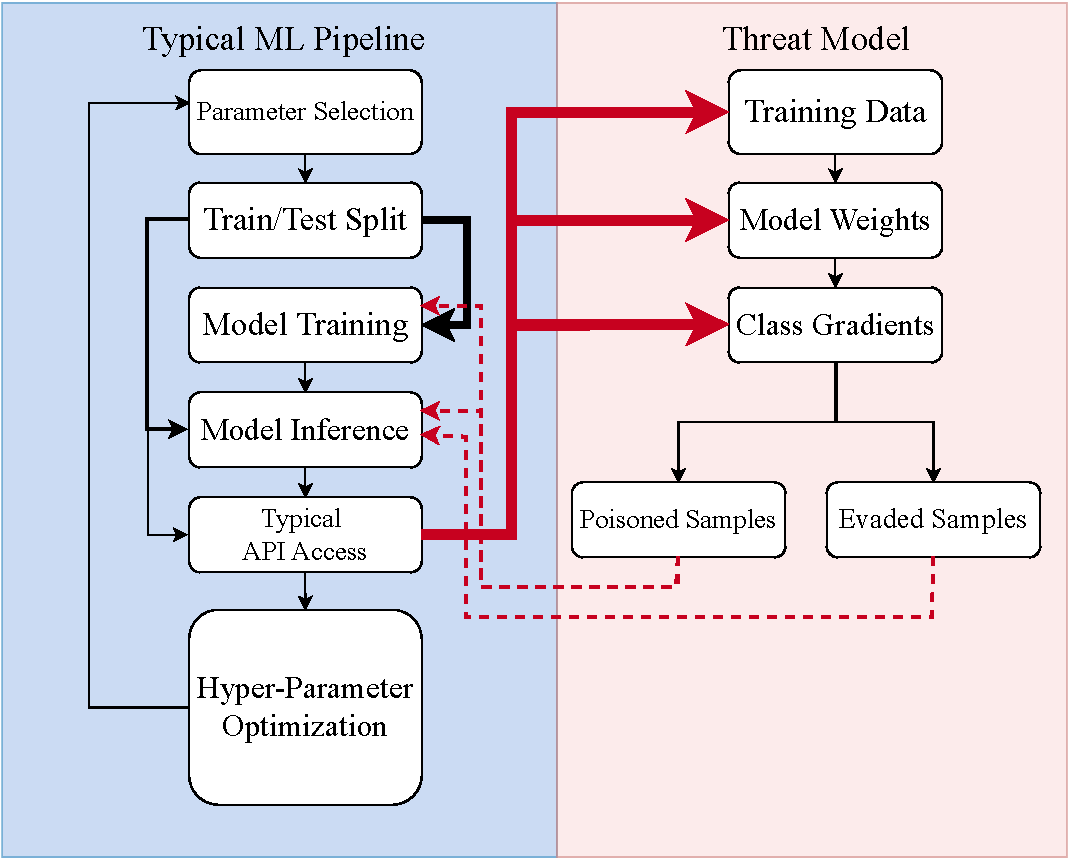
\includegraphics[width=.6\textwidth]{images/attack_diagram.pdf}
%     \caption{This diagram depicts the various threat models against a typical machine learning model. The blue box depicts the typical ML pipeline training process and the red box reveals how each part of the model pipeline can be targeted by an adversary. The solid black lines follow the flow of data within either the benign (blue) or adversarial (red) pipelines. The solid red lines indicate what kinds of data can be extracted via typical API access and the dotted red lines reveal the kinds of data that can be inserted into a ML pipeline by an adversary. Even if an adversary has}
%     \label{fig:threat_model}
% \end{figure*}
% \label{threat}

% \subsection{Attacks}
% \label{attacks}
% \begin{itemize}
%     \item FGM
%     \item HSJ


% \end{itemize}
% \subsubsection{Attack Related Metrics}
% \paragraph{Minimal Evasion Distance}
% \paragraph{Survival Time}
% % \pargraph{KL_Divergence}
% \paragraph{SHAPr Privacy Metric}
\section{Run-Time Improvements}
\label{improvements}
We can use this model in two different paradigms. In general, the idea is that the number of requisite training samples is very small, so we can run everything client-side, keeping the particulars of the model training private. Another method for distributing the training process, federated learning, trains a model for each user but routinely shares model weights upstream to create a better model for everyone. However, as we outlined in Sec.~\ref{threat}, that opens new attack vectors that would be unsuitable for information the user would like to keep private (\textit{e.g.}, IP address, message contents, or schedule of use). Instead, we propose a few-shot and online methodology for re


\subsection{Real-time, Anomaly Detection}
In some situations, it might be necessary to find anomalies in real-time, which involves special considerations. Namely, we can skip the "training" step entirely and select a number of existing samples from our database for training. These could be selected randomly or according to some time filter in an attempt to only capture new or otherwise unnoticed anomalies. In some cases, it may be that the user doesn't have many samples. However, as we show in the Sec.~\ref{results}, that even small training sets are remarkably effective for this method.



%  Numeric Distances
% \begin{itemize}
%     \item $\ell_0$ (bit-wise distance)
%     \item $\ell_1$ (taxi-driver distance)
%     \item $\ell_2$ (euclidean)
%     \item $\mathscr{\chi}^2$ (weighted difference per entry)
%     \item $\mathscr{L}$ (Laplacian)
%     \item $\mathscr{W}$ (Wasserstein)
% \end{itemize}

\subsubsection{Calculating the Gram matrix}
\label{symmetry}
While many of the above distance metrics are symmetric, this is not-necessarily the case with NCD. 
However, if we assume this is true most of the time, we can reduce the computational cost of training. Below, we have tested two separate modifications of the ``vanilla'' NCD algorithm. 
The first modification involves assumed symmetry. 
By sorting the values $x,y$ first by length then alphabetically (Algorithm~\ref{alg:enforced_symmetry}), we ensure that $d(x,y) > 0$ in at least some cases where the $ C(xy) < \min\{C(x),C(y)\}$. However, there are some cases that are not covered, particularly.

Section~\ref{results} shows how this often improves the accuracy of a model and reduces the number of calculations required to find the distance matrix.

\begin{algorithm}
    \begin{algorithmic}
        \Require $X_1$, $X_2$, indexed by $i,j$ respectively
        \Ensure $ \| X_1 \| = \| X_2 \| $
        \State $K_{i,j} \gets 0$ for all $i, j$
        \If{x< y}
        \State{$x,y \gets y,x$}
        \ForAll{pairs of indices $(i, j) \in \mathcal{D}(X_1, X_2)$ such that $i < j + 1$}
            \State $\mathcal{D}_{ij} \gets \mathcal{D}(X_{1_i}, X_{2_j})$
            \State $S_{ij} \gets \mathcal{D}_{ij}$
            \State $S_{ji} \gets \mathcal{D}_{ij}$
        \State \textbf{Output:} Symmetric distance matrix $S$
    \end{algorithmic}
    \caption{Compute the \textit{Assumed} Symmetric Distance Matrix. \cm{This differs from the below in that symmetry is assumed to be true rather than enforced.}}
    \label{alg:assumed_symmetry}
\end{algorithm}

\begin{algorithm}
    \begin{algorithmic}
        \Require $X_1$, $X_2$, indexed by $i,j$ respectively
        \Ensure $ \| X_1 \| = \| X_2 \| $
        \State $K_{i,j} \gets 0$ for all $i, j$
        \If{x< y}
        \State{$x,y \gets y,x$}
        \ForAll{pairs of indices $(i, j) \in \mathcal{D}(X_1, X_2)$ such that $i < j + 1$}
            \State $\mathcal{D}_{ij} \gets \mathcal{D}(X_{1_i}, X_{2_j})$
            \State $S_{ij} \gets \mathcal{D}_{ij}$
            \State $S_{ji} \gets \mathcal{D}_{ij}$
        \State \textbf{Output:} Symmetric distance matrix $S$
    \end{algorithmic}
    \caption{Compute the \textit{Enforced} Symmetric Distance Matrix. \cm{The Modified algorithm does two things, return 0 if x = y and sorts the strings so that ncd(x,y) is symmetric with the longer one going first. This solves the negativity problem. TODO: Fix latex}}
    \label{alg:enforced_symmetry}
\end{algorithm}



% \subsubsection{Pre-computing the Compression vector}
% Since the compression step requires the most processing time, we can pre-compute the compression distance for our input data as part of a training step, if we so choose. This offers marginal run-time improvements over the original implementation that repeatedly calculated the NCD of all training samples for each example in the test set. 
% See Fig.~\ref{fig:sym_train_time} to see the (signficant) decrease in run-time  and the resulting (marginal) change in accuracy when we pre-compress all of the train and test strings in the data. %Note: this is still running. 










\subsubsection{Reducing the Search Space}
\label{condensing_methods}
In other situations, it is necessary to minimise the number of samples used for evaluation because the size of the user's database is too large to evaluated in a reasonable amount of time. We can use a variety of heuristics to reduce the size of our training set~\cite{amal2011survey} as an attempt to overcome the run-time constraints described in Section~\ref{ncd-knn}.



\begin{algorithm}
  \caption{Find M-Best Indices (Condensing)}
  \label{alg:m-best-indices}
  \begin{algorithmic}
    \State \textbf{Input:} Sample points $X$, number of best indices $m$
    \State \textbf{Output:} Set of indices $I$ containing the $m$-best points
    \ForAll{$x$ in $X$}
      \State Compute relevance score $r_x$ based on a given criterion
    % \EndFor
    \State $I \gets \text{sortIndices}(r_x)$
    \State \Return top $m$ indices in $I$
  \end{algorithmic}
\end{algorithm}


% \subsubsection{Iterative Methods}
% We can now treat this as an iterative problem and do a continuous hyperparameter search.


% \begin{algorithm}
%   \caption{Model Training}
%   \label{alg:condensing}
%   \begin{algorithmic}
%     \Require System state $S$, Number of iterations $N$, Number of best indices $m$, $x_{test}, y_{test}, X_{train}, y_{train}$
%     \State \textbf{Output:} Final system state $S$
%     \State Initialize system: $S \gets$ baseline state
%     \For{$i = 1$ to $N$}
%       \State Sample points: $P \gets \text{samplePoints}(S)$
%       \State Find m-best indices: $I \gets \text{findMBestIndices}(P, m)$
%     \State \Return $m$-best indices, $I$
%   \end{algorithmic}
% \end{algorithm}






\section{Methods}
Broadly, this section is divided into two sets of experiments. First, we tuned each model to each dataset while examining the effect of sample size and the effect of modified algorithm (see:~\ref{symmetry}). Then, after confirming the $\mathcal{O}(nm)$ runtime for number of testing, training samples $n,m$, we examine the effect of various training set condensing methods to reduce the run-time. 


% Next steps:
% Online training with condensing? Or is this just an application we can mention, calling the implementation `out of scope'
% Another dataset? Truthseeker is really bad (Twiitter is actually just very spammy and the dataset abels were made up in like 2012). Could be replaced or contextualized with a better, but similar dataset
%  Examine the degree to which the metric space assumptions are violated
% Compare the privacy/attack-ability using the SHAPr metric, but what's the baseline here? A NN? A KNNs/SVCs/Logistic Models that use something other than gzip as a tokenizer (e.g. Word2Vec). My strong suspcion is that you'll get more bits per sample from word2vec than from gzip since the latter only returns a number and not a vector of tokens.
% As of 27/7, I'm leaning towards the SHAPr metric, since that can be implemented rather quickly on, for example, the best model (but tested on a new random permutations than during training). I should know by 29/7 if this is going to go anywhere
\label{methods}
\subsection{Datasets}
\label{datasets}
We examine several to show that this method works well for a variety of anomaly-detection tasks. The `normal' data were under-sampled so that there was an equal number of normal and anomalous samples. For several of the datasets, anomalies were rare. 
To overcome the limitation of getting a precise measure of accuracy on a small number of samples, Monte Carlo sampling was employed by testing each configuration across 10 random permutations of the data. 
This is known to be asymptotically equivalent to cross-fold validation~\cite{shan2022monte} which is not remotely precise enough when we have only a small number of anomalous data points. 
Additionally, the test and train sets were sampled in such a way that each configuration was guaranteed to have a uniform distribution of the classes in both sets. To examine the efficacy of this method on numeric, string, and heterogeneous datasets, several standard datasets were examined. 
The oldest one is KDD-NSL which is a log of system process data for both regular users (labelled 0 or benign) and malicious users (labelled 1 or adversarial)~\cite{kddnsl}. The DDoS IoT dataset ~\cite{ddos} was also included. 
To prepare this dataset, we combined all classes of attacks with the non-malicious user data, collapsing all attacks into the adversarial (1) label. In addition, the timestamp data was removed to prevent data leakage  (since the malicious and benign data were collected sequentially). 
Then, in an effort to examine the efficacy of this on text alone, the Truthseeker ~\cite{truthseeker} was used. While this is normally distributed with metadata, this work only included the ``tweet" and the label provided by the researchers who distribute the data (again, a 0 or 1 corresponding to a regular or malicious user respectively). 
To examine more heterogeneous data, the SMS Spam dataset was chosen. 
This combines a short text message with numeric and protocol data to again distinguish between regular SMS messages (labelled with a 0) and spam ones (labelled with a 1). 

\subsection{Models}

After generating 1000 train/test set pairs for each dataset, the distance matrices were calculated and provided to typical \texttt{scikit-learn} classifiers. For each compression algorithm or string metric, both the symmetric (as per  Alg. \ref{alg:assumed_symmetry}) and asymmetric matrices were found and tested. Since these models have several parameters, some of which are drawn from continuous spaces, we used a Tree Parzen Estimator~\cite{tpe} to tune each model for each distance metric. For each hyper-parameter configuration trials were conducted across 

The test hyper-parameters are listed below.

\label{models}
\subsubsection{$k$-KNN}
To use KNN, one must specify a number of nearest neighbours to use for class prediction (see: Algorithm~\ref{alg:knn}). This number was selected from $\{1,3,5,7,11\}$, as choosing small, odd numbers to make ties impossible for binary classifiers. In addition, we tested whether or not to weight the samples uniformly or by distance. 

\subsubsection{$k$-SVC}
Ths \texttt{scikit-learn} SVC implementation provides several kernel methods for transforming the input into a separable feature space. 
For the sake of simplicity, only the radial basis function (RBF) was tested (it's also known to be a universal function approximator~\cite{}). 
SVCs require a choice of value for a penalty term and we tested the range $[ 10^{-3}, 10^3]$ and let \texttt{scikit-learn} choose an apporpriately sized $\gamma$ parameter for the RBF function. 
The "balanced" and null class weight parameters that control the relative importance of a sample were also tested.

\subsubsection{$k$-Logistic}
The \texttt{scikit-learn} provides several parameters for the humble logistic function. Both an $\ell_1$ and $\ell_2$ penalty term were tested as well as a configuration without a penalty. That penalty was sampled from the range $[10^{-3}, 10^3]$. In addition, logistic models with and without intercept parameters were tested. Using the \texttt{saga} solver, we tested stopping criteria tolerances $\in [10^{-4}, 10^{-2}]$
As with the SVC above, the "balanced" and null class weight parameters that control the relative importance of a sample were also tested.

\subsection{Compressors}
\label{compressors}
In addition to \texttt{gzip}, we tried numerous different compression algorithms. We used the \texttt{gzip}, \texttt{lzma}, \texttt{bz2}, and \texttt{zst} python modules with default arguments. A comparison of these algorithms can be seen in Table~\ref{tab:compression_algorithms}.

\subsection{Condensing}
\label{condensing}
We provide theoretical justifications for using secondary methods for determining ideal training set in Section~\ref{improvements}. The mean, medoid, random, \textit{KNN}, and \textit{SVC} methods were used to select the $m$-most important samples for each with $m \in$ [10,20,50,100,200,500,900]. The methods are outlined in full in Sec.~\ref{condensing_methods}. For the KNN and medoid, we used \texttt{imblearn}, a \texttt{scikit-learn} compatible package for using various condensing methods. The \texttt{scikit-learn} implementation was used for \textit{SVC}. For \textit{random} and \textit{sum}, \texttt{numpy} implementations were used.

\begin{itemize}
    \item \textit{Sum:} After calculating the distance matrix, we sort the distance matrix by the sum of a row and find the $m$ most central samples per class.
    \item \textit{Medoid: }
    \item \textit{Random : } After calculating the distance matrix, we select $m$ random indices per class.
    \item \textit{KNN: } After calculating the distance matrix, we use the KNN algorithm to find the $m$-closest neighbors for each class in the training data.
    \item \textit{SVC: } After calculating the distance matrix, we use a support vector classifier (SVC) to find the indices that define the support-vectors (e.g. the samples that define the class boundaries), then we sort by distance as in \textit{Sum} to find the $m$-most central support vectors to use during the prediction step.
\end{itemize}

\section{Results}
\label{results}


% \subsection{Kernelized Classifier Performance}
% \begin{figure*}[htb]
%     \centering
%     \begin{subfigure}[htb]{\textwidth}
%         \centering
%         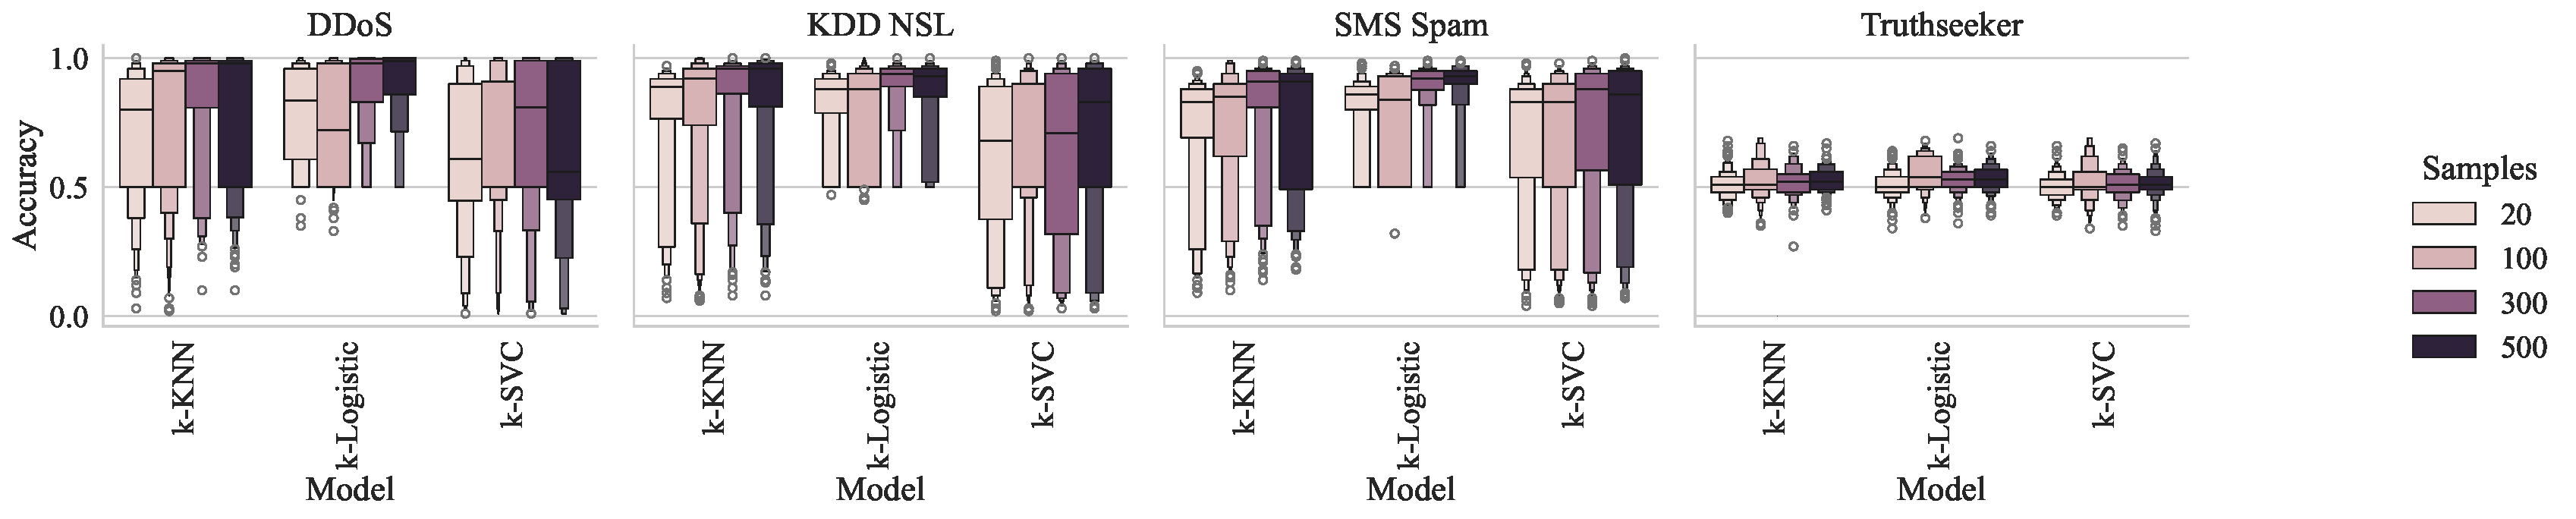
\includegraphics[width=\textwidth]{figs/combined/models_vs_accuracy.pdf}
%         \caption{Accuracy across models and datasets.}
%         \label{fig:acc_summary}
%     \end{subfigure}
%     \begin{subfigure}[htb]{\textwidth}
%         \centering
%         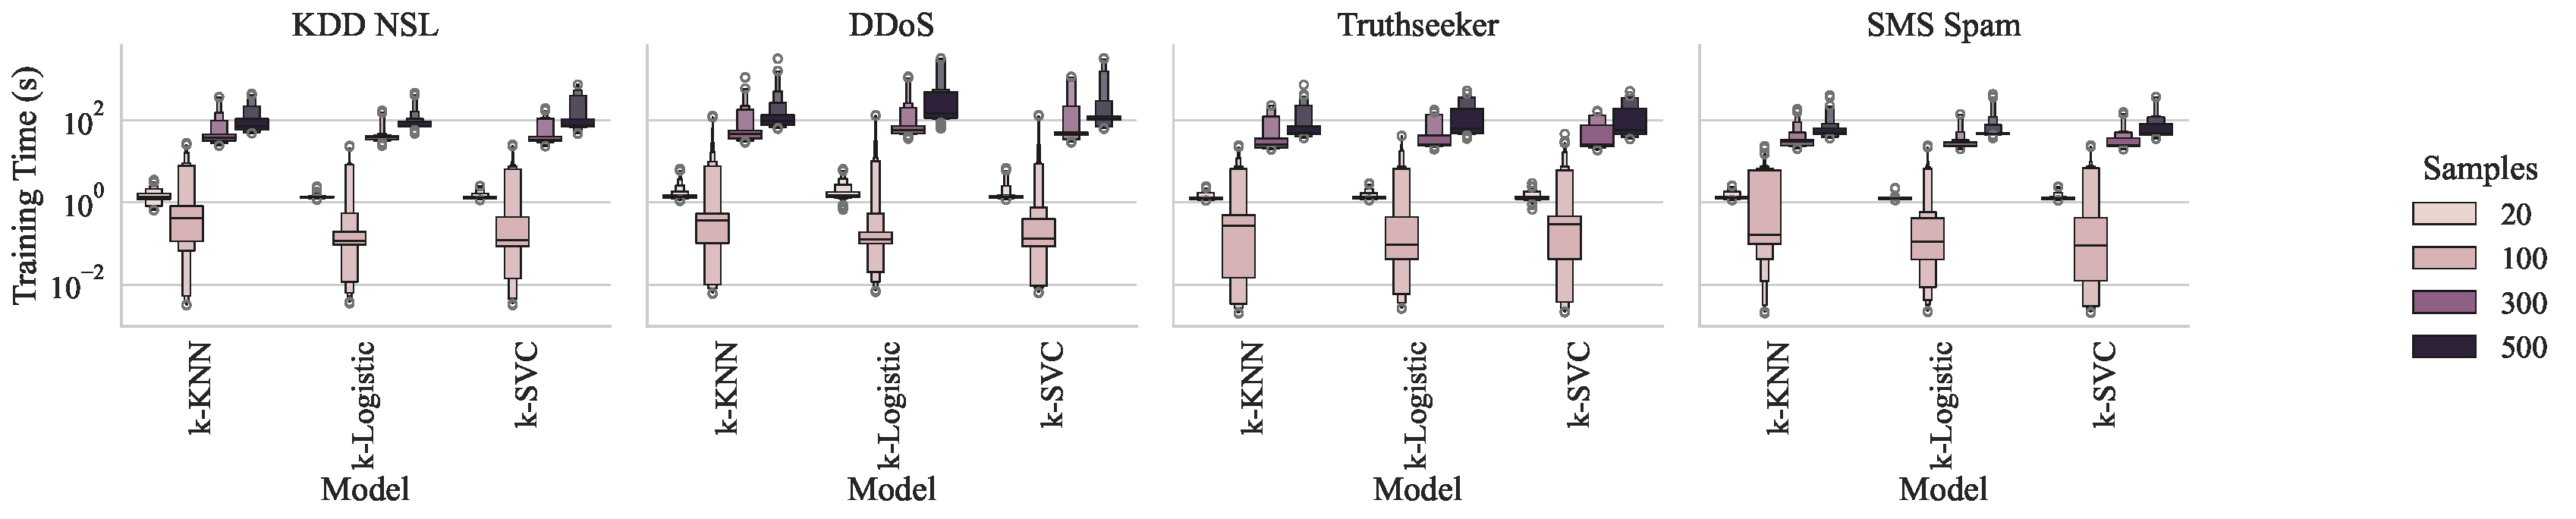
\includegraphics[width=\textwidth]{figs/combined/models_vs_train_time.pdf}
%         \caption{Training Time across models and datasets.}
%         \label{fig:train_time_summary}
%     \end{subfigure}
%     \begin{subfigure}[htb]{\textwidth}
%         \centering
%         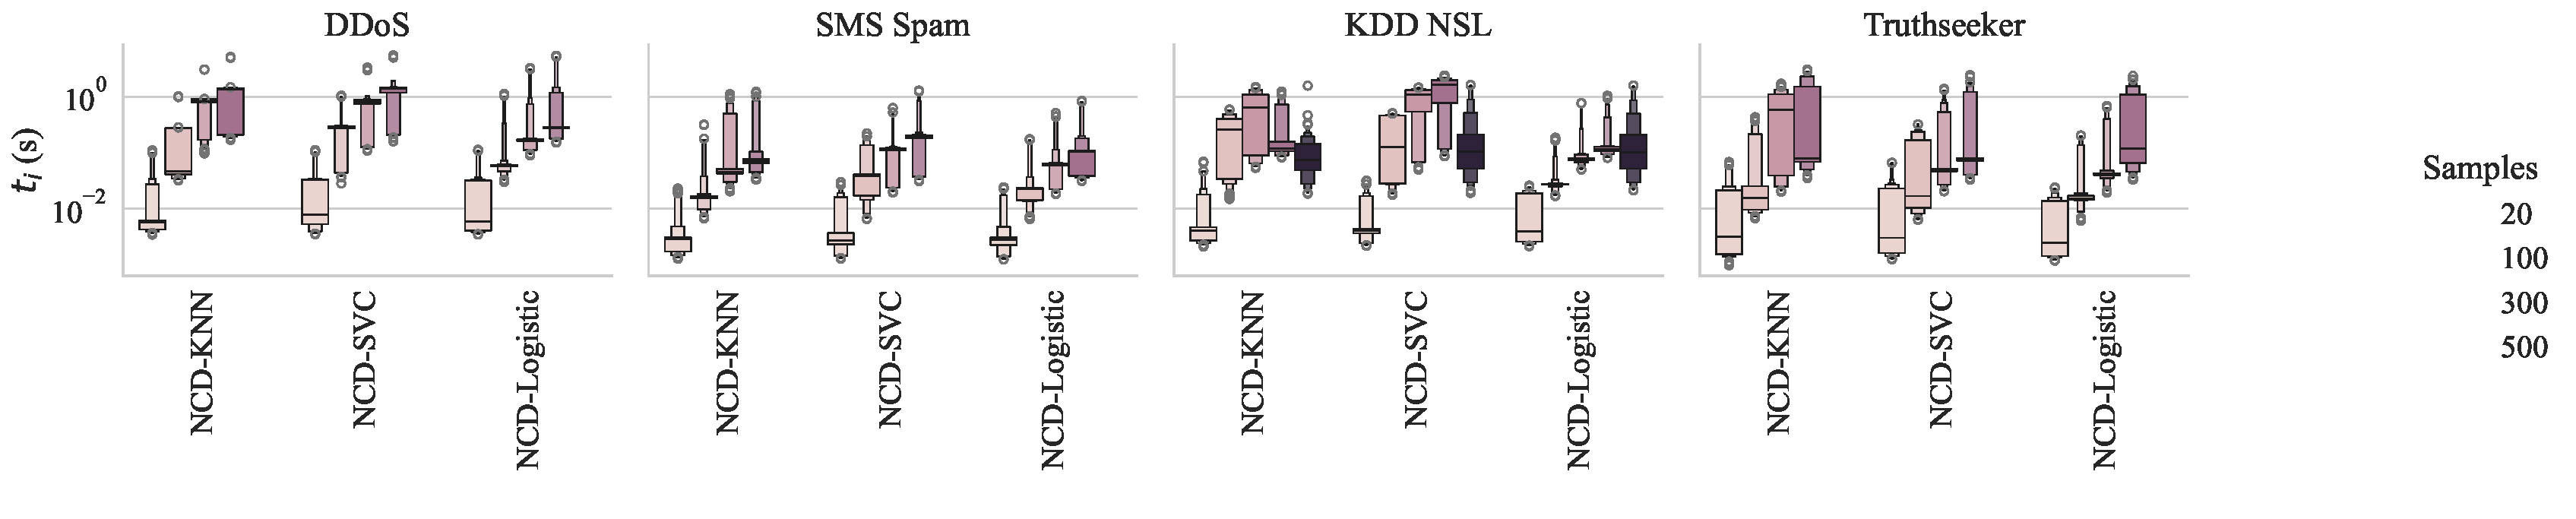
\includegraphics[width=\textwidth]{figs/combined/models_vs_predict_time.pdf}
%         \caption{Prediction Time across models and datasets.}
%         \label{fig:pred_time_summary}
%     \end{subfigure}
%     \caption{Kernelized classifier performance across many datasets, models, and sample sizes. Each column corresponds to a different dataset and each row corresponds to a different performance metric, the value of which is on the y-axis. The x-axis in each plot corresponds to a classifier type and the colour conveys the number of samples provided during training.}
%     \label{fig:sample_summary}
% \end{figure*}


% \lipsum[1]~\ref{fig:sample_summary}

% \subsection{Effect of Symmetry Assumption}



% \begin{figure*}[htb]
%     \centering
%     \begin{subfigure}[htb]{\textwidth}
%         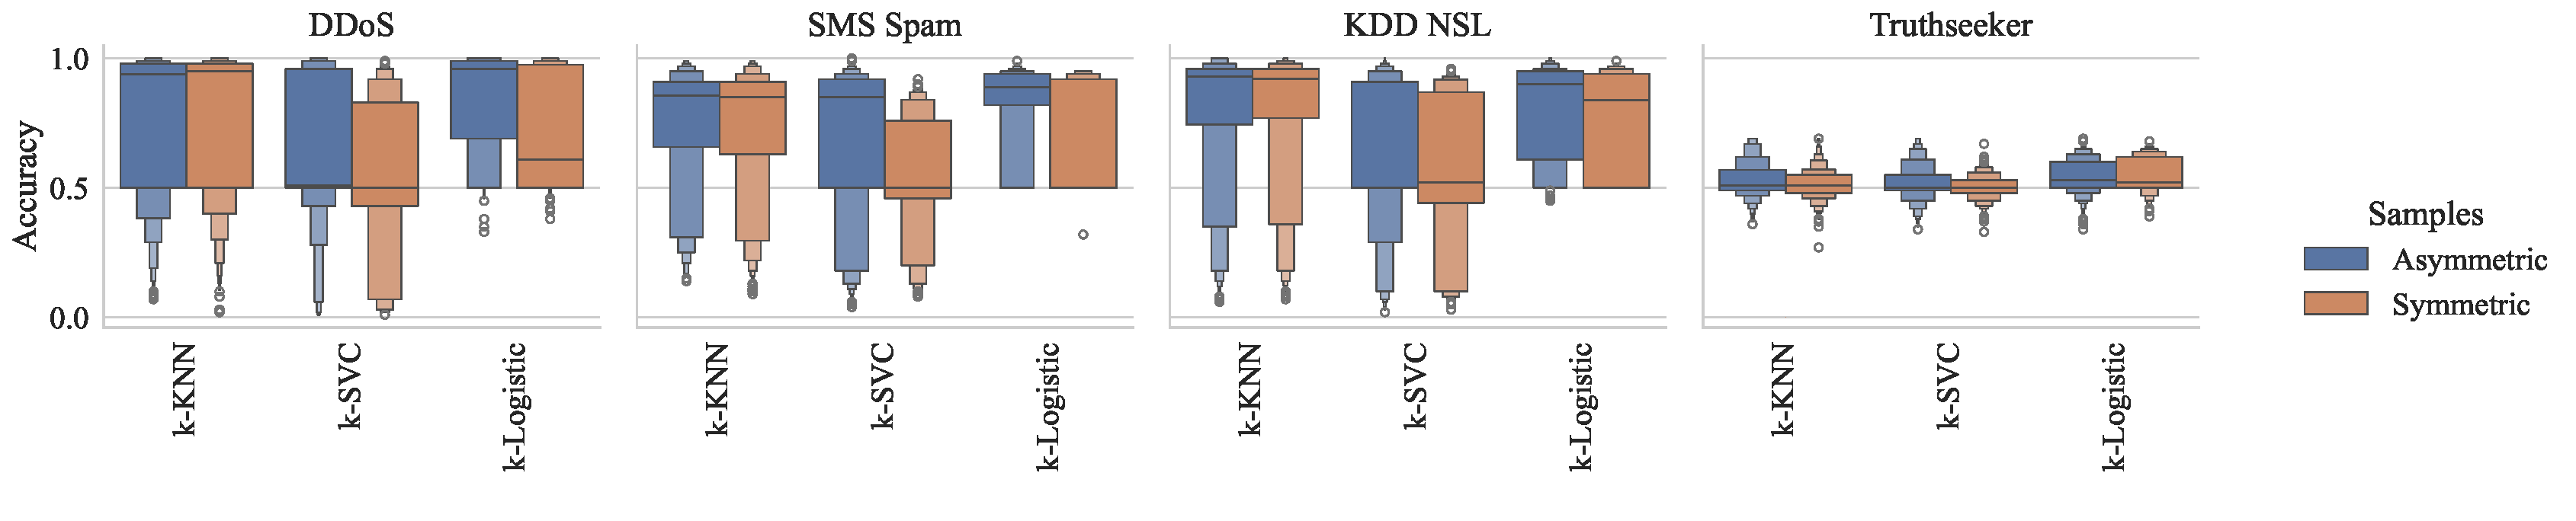
\includegraphics[width=\textwidth]{figs/combined/symmetric_models_vs_accuracy.pdf}
%         \caption{Accuracy across models and datasets.}
%         \label{fig:symm_acc}
%     \end{subfigure}
%     \begin{subfigure}[htb]{\textwidth}
%         \centering
%         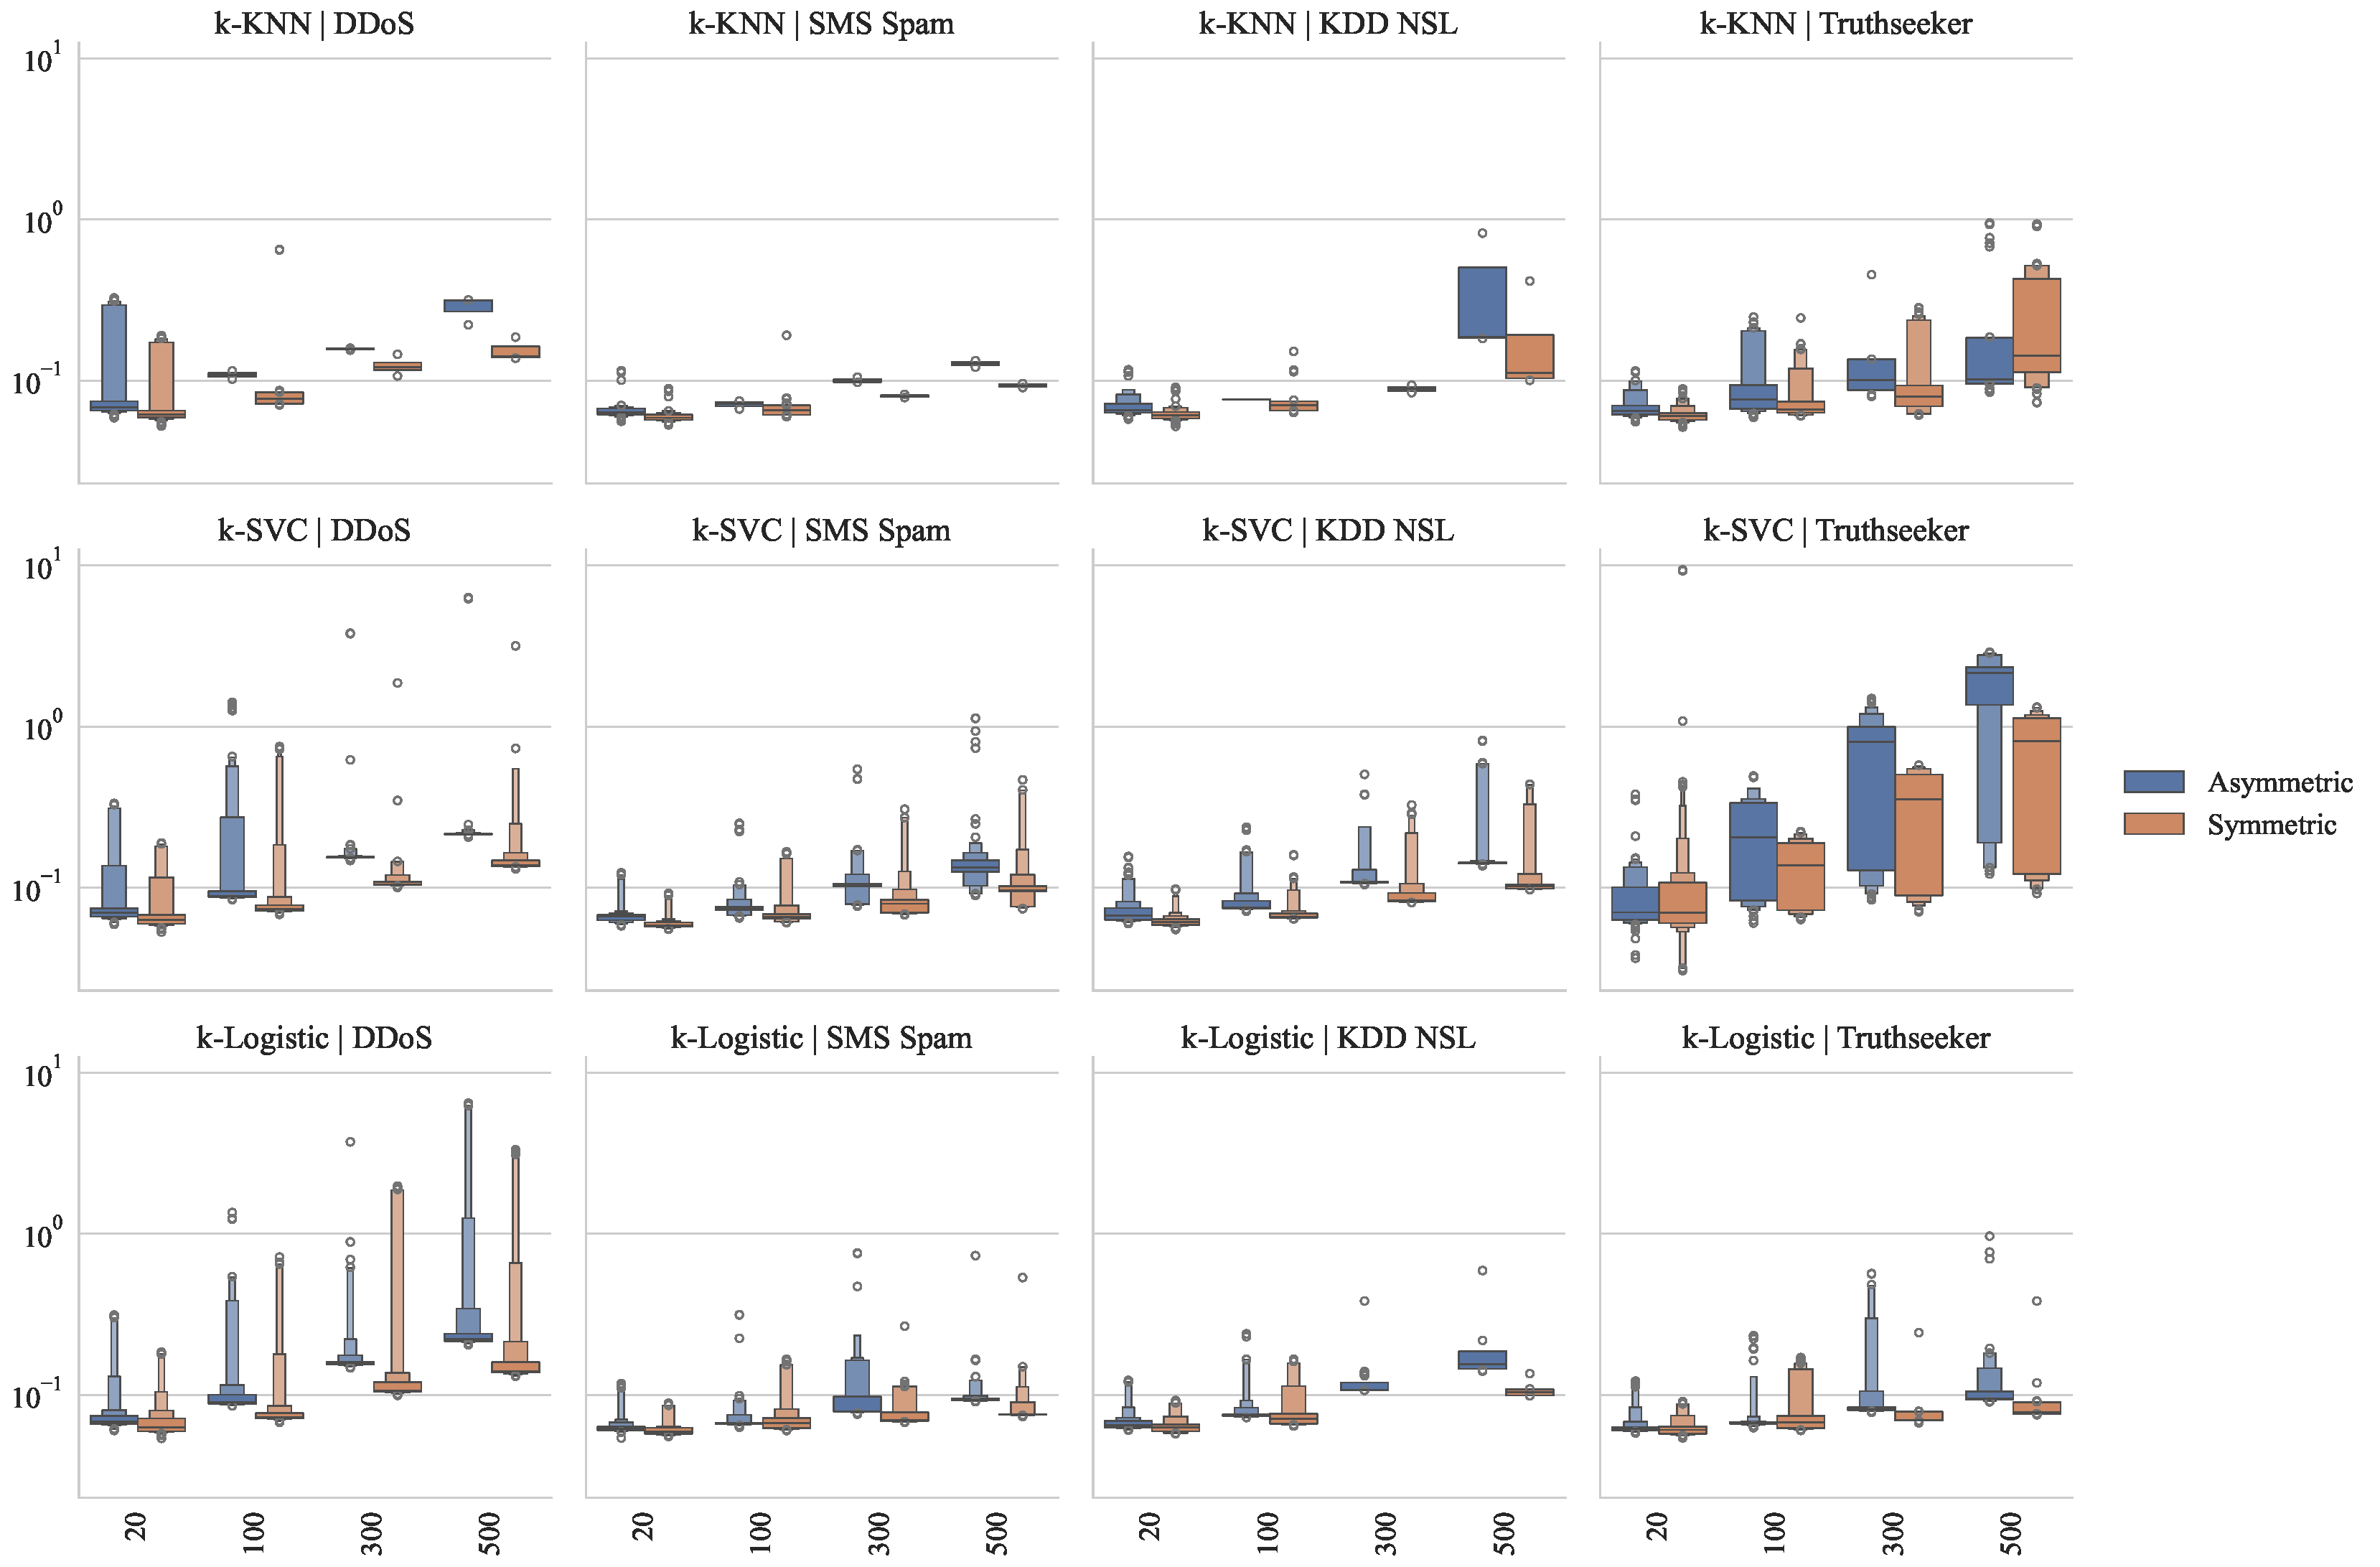
\includegraphics[width=\textwidth]{figs/combined/symmetric_models_vs_train_time.pdf}
%         \caption{Training Times across models and datasets.}
%         \label{fig:sym_train_time}
%     \end{subfigure}
%     \begin{subfigure}[htb]{\textwidth}
%         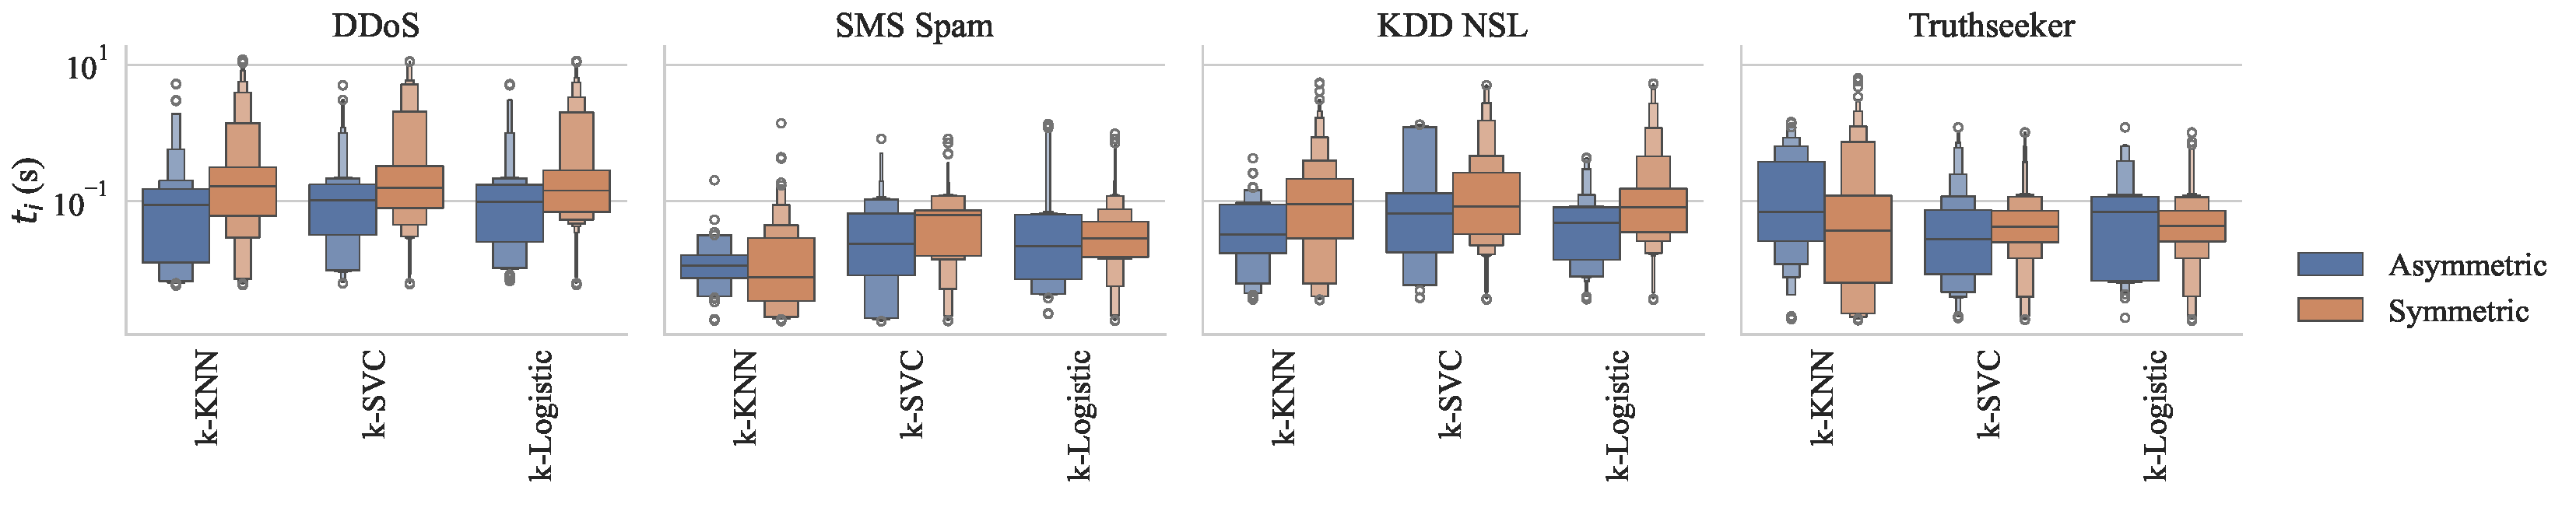
\includegraphics[width=\textwidth]{figs/combined/symmetric_models_vs_predict_time.pdf}
%         \caption{Prediction Times across models and datasets.}
%         \label{fig:sym_pred_time}
%     \end{subfigure}
%     \caption{Kernelized classifier inference times across many datasets, and models while examining the effect of the symmetric assumption outlined in Algorithm~\ref{alg:assumed_symmetry}. Each column corresponds to a different dataset and each row corresponds to a different performance metric, the value of which is on the y-axis. The x-axis in each plot corresponds to a classifier type and the colour conveys whether symmetry was assumed (orange) or not (blue).}
%     \label{fig:symm_summary}
% \end{figure*}

% \lipsum[1]~\ref{fig:symm_summary}

\subsection{Comparison of Different String Metrics}
\begin{figure*}[htb]
    \centering
    \begin{subfigure}[htb]{\textwidth}
        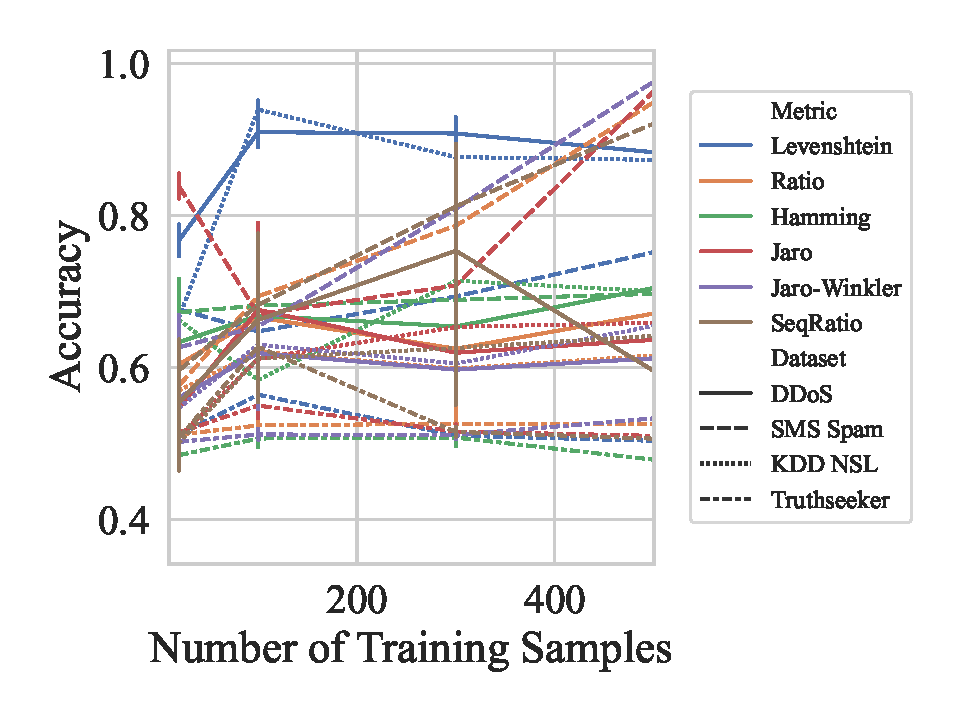
\includegraphics[width=.45\textwidth]{figs/combined/string_metric_vs_accuracy.pdf}
        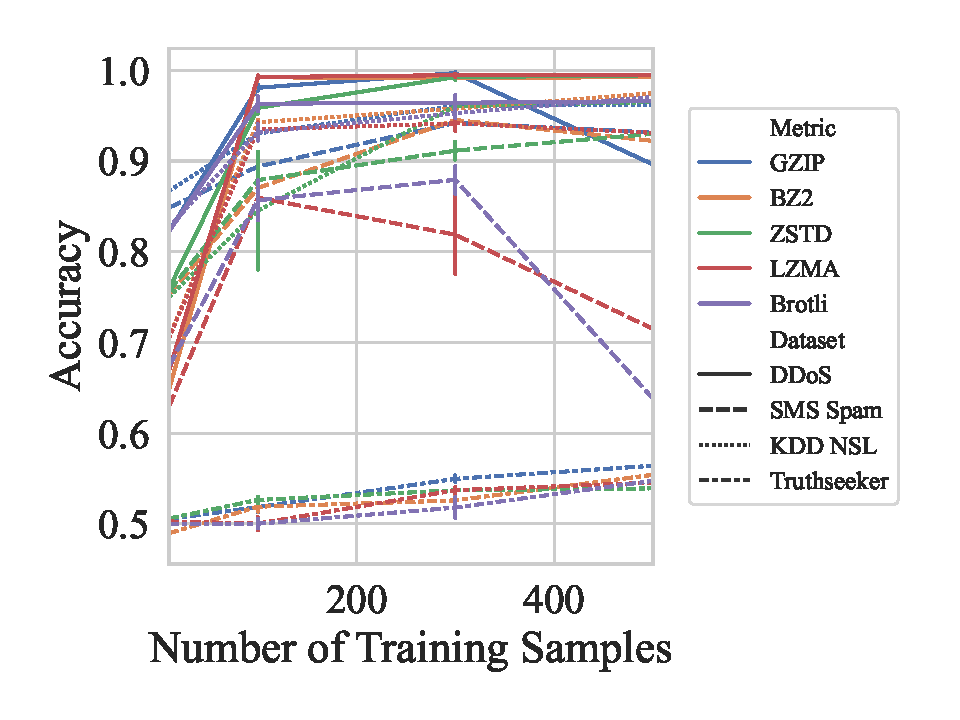
\includegraphics[width=.45\textwidth]{figs/combined/compressor_metric_vs_accuracy.pdf}
    \end{subfigure}
    
    \begin{subfigure}[htb]{\textwidth}
        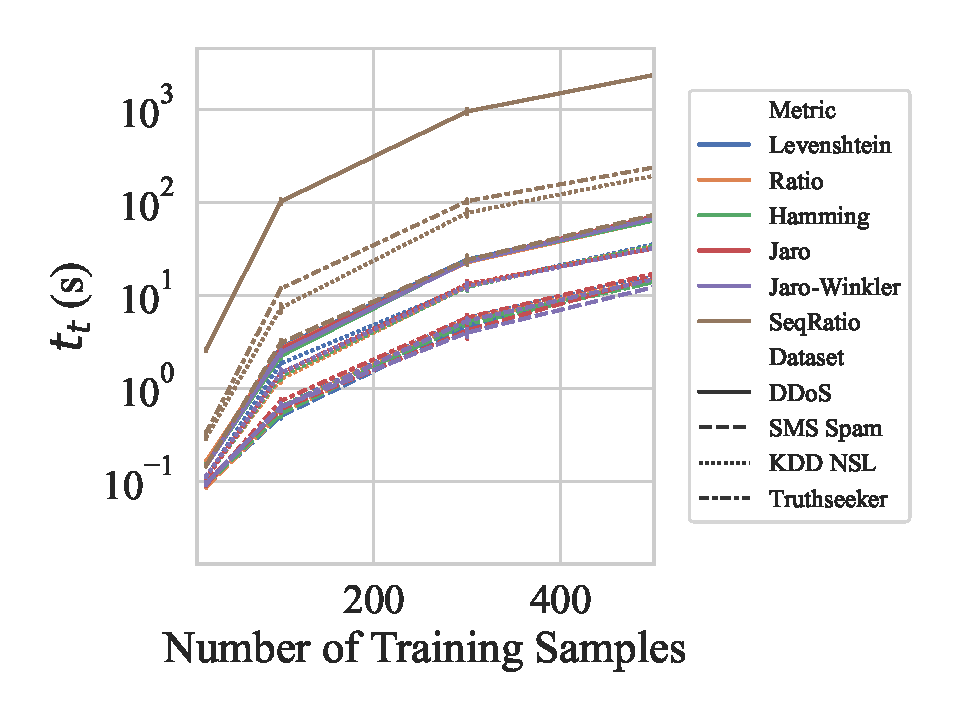
\includegraphics[width=.45\textwidth]{figs/combined/string_metric_vs_train_time.pdf}
        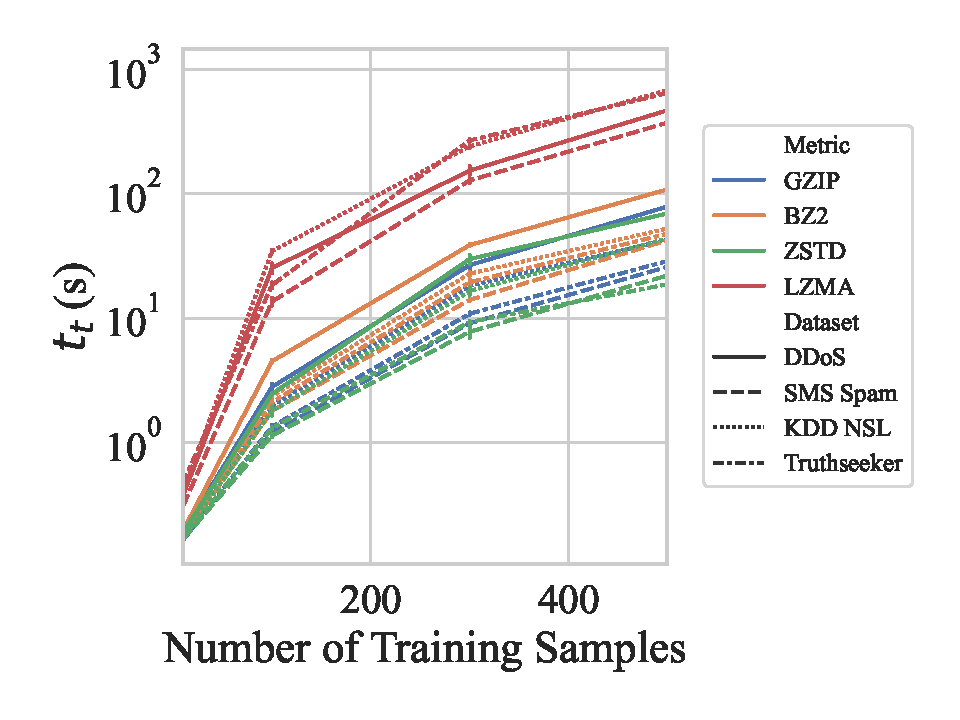
\includegraphics[width=.45\textwidth]{figs/combined/compressor_metric_vs_train_time.pdf}
    \end{subfigure}
   
    \begin{subfigure}[htb]{\textwidth}
        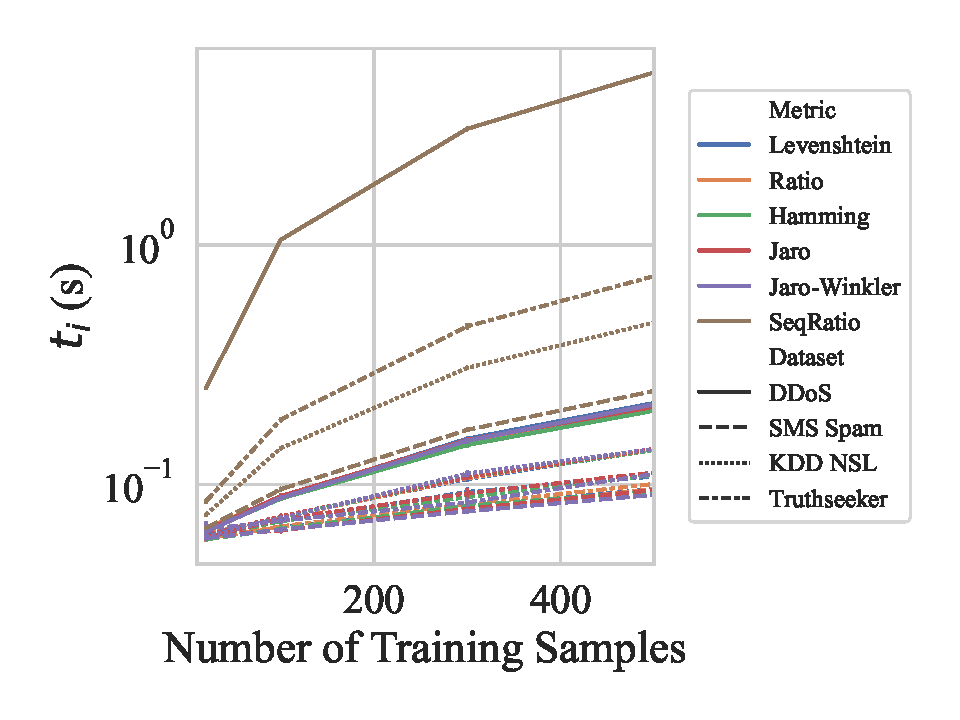
\includegraphics[width=.45\textwidth]{figs/combined/string_metric_vs_predict_time.pdf}
        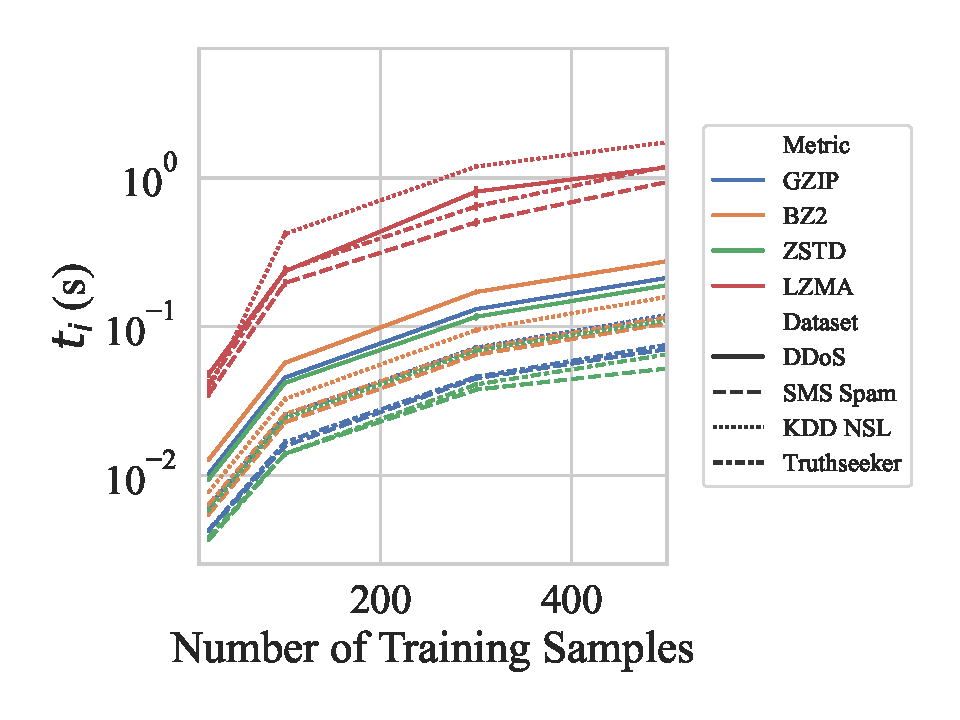
\includegraphics[width=.45\textwidth]{figs/combined/compressor_metric_vs_predict_time.pdf}
    \end{subfigure}
    
    \caption{Kernelized classifier accuracy (top), training times (middle), and inference times (bottom) across many datasets (style), and models. The left column depicts the results from the tested string metrics (see: Section~\ref{string_metrics}) and the right side depicts the results from the modified NCD algorithm using various compressors (see: Section~\ref{compressors})}
    \label{fig:models_summary}
\end{figure*}

Figure~\ref{fig:models_summary} shows the performance of the various classifiers (knn, logistic, SVC) across each of the datasets using various string metrics (left column) and compressors (right column) to calculate NCD. We see that run-times are largely comparable between NCD and various string metrics for both training ($t_t$) and inference ($t_i$). 
However, NCD provides consistently more accurate results with a small number of samples, apart from Levenshtein distance which works quite well with 10s of samples. 
Please note that the training step is only necessary for certain configurations of the KNN algorithm and that the vanilla version proposed by Jiang et. al.~\cite{jiang2022less} can skip this step entirely. However, Figure~\ref{fig:mod_acc} shows that kernelized SVCc and Logistic Regressors can offer improved accuracy over this "untrained" version.
However, As we increase the number of samples, Jaro, Waro-Winkler, and seqratio become more useful for the SMS dataset, but remain unremarkable for the other datasets. Overall, NCD offers superior performance over the tested string metrics since it performs consistently well across all of the datasets. 


\subsection{Effect of Modified NCD Algorithm}

\begin{figure*}[htb]
    \centering
    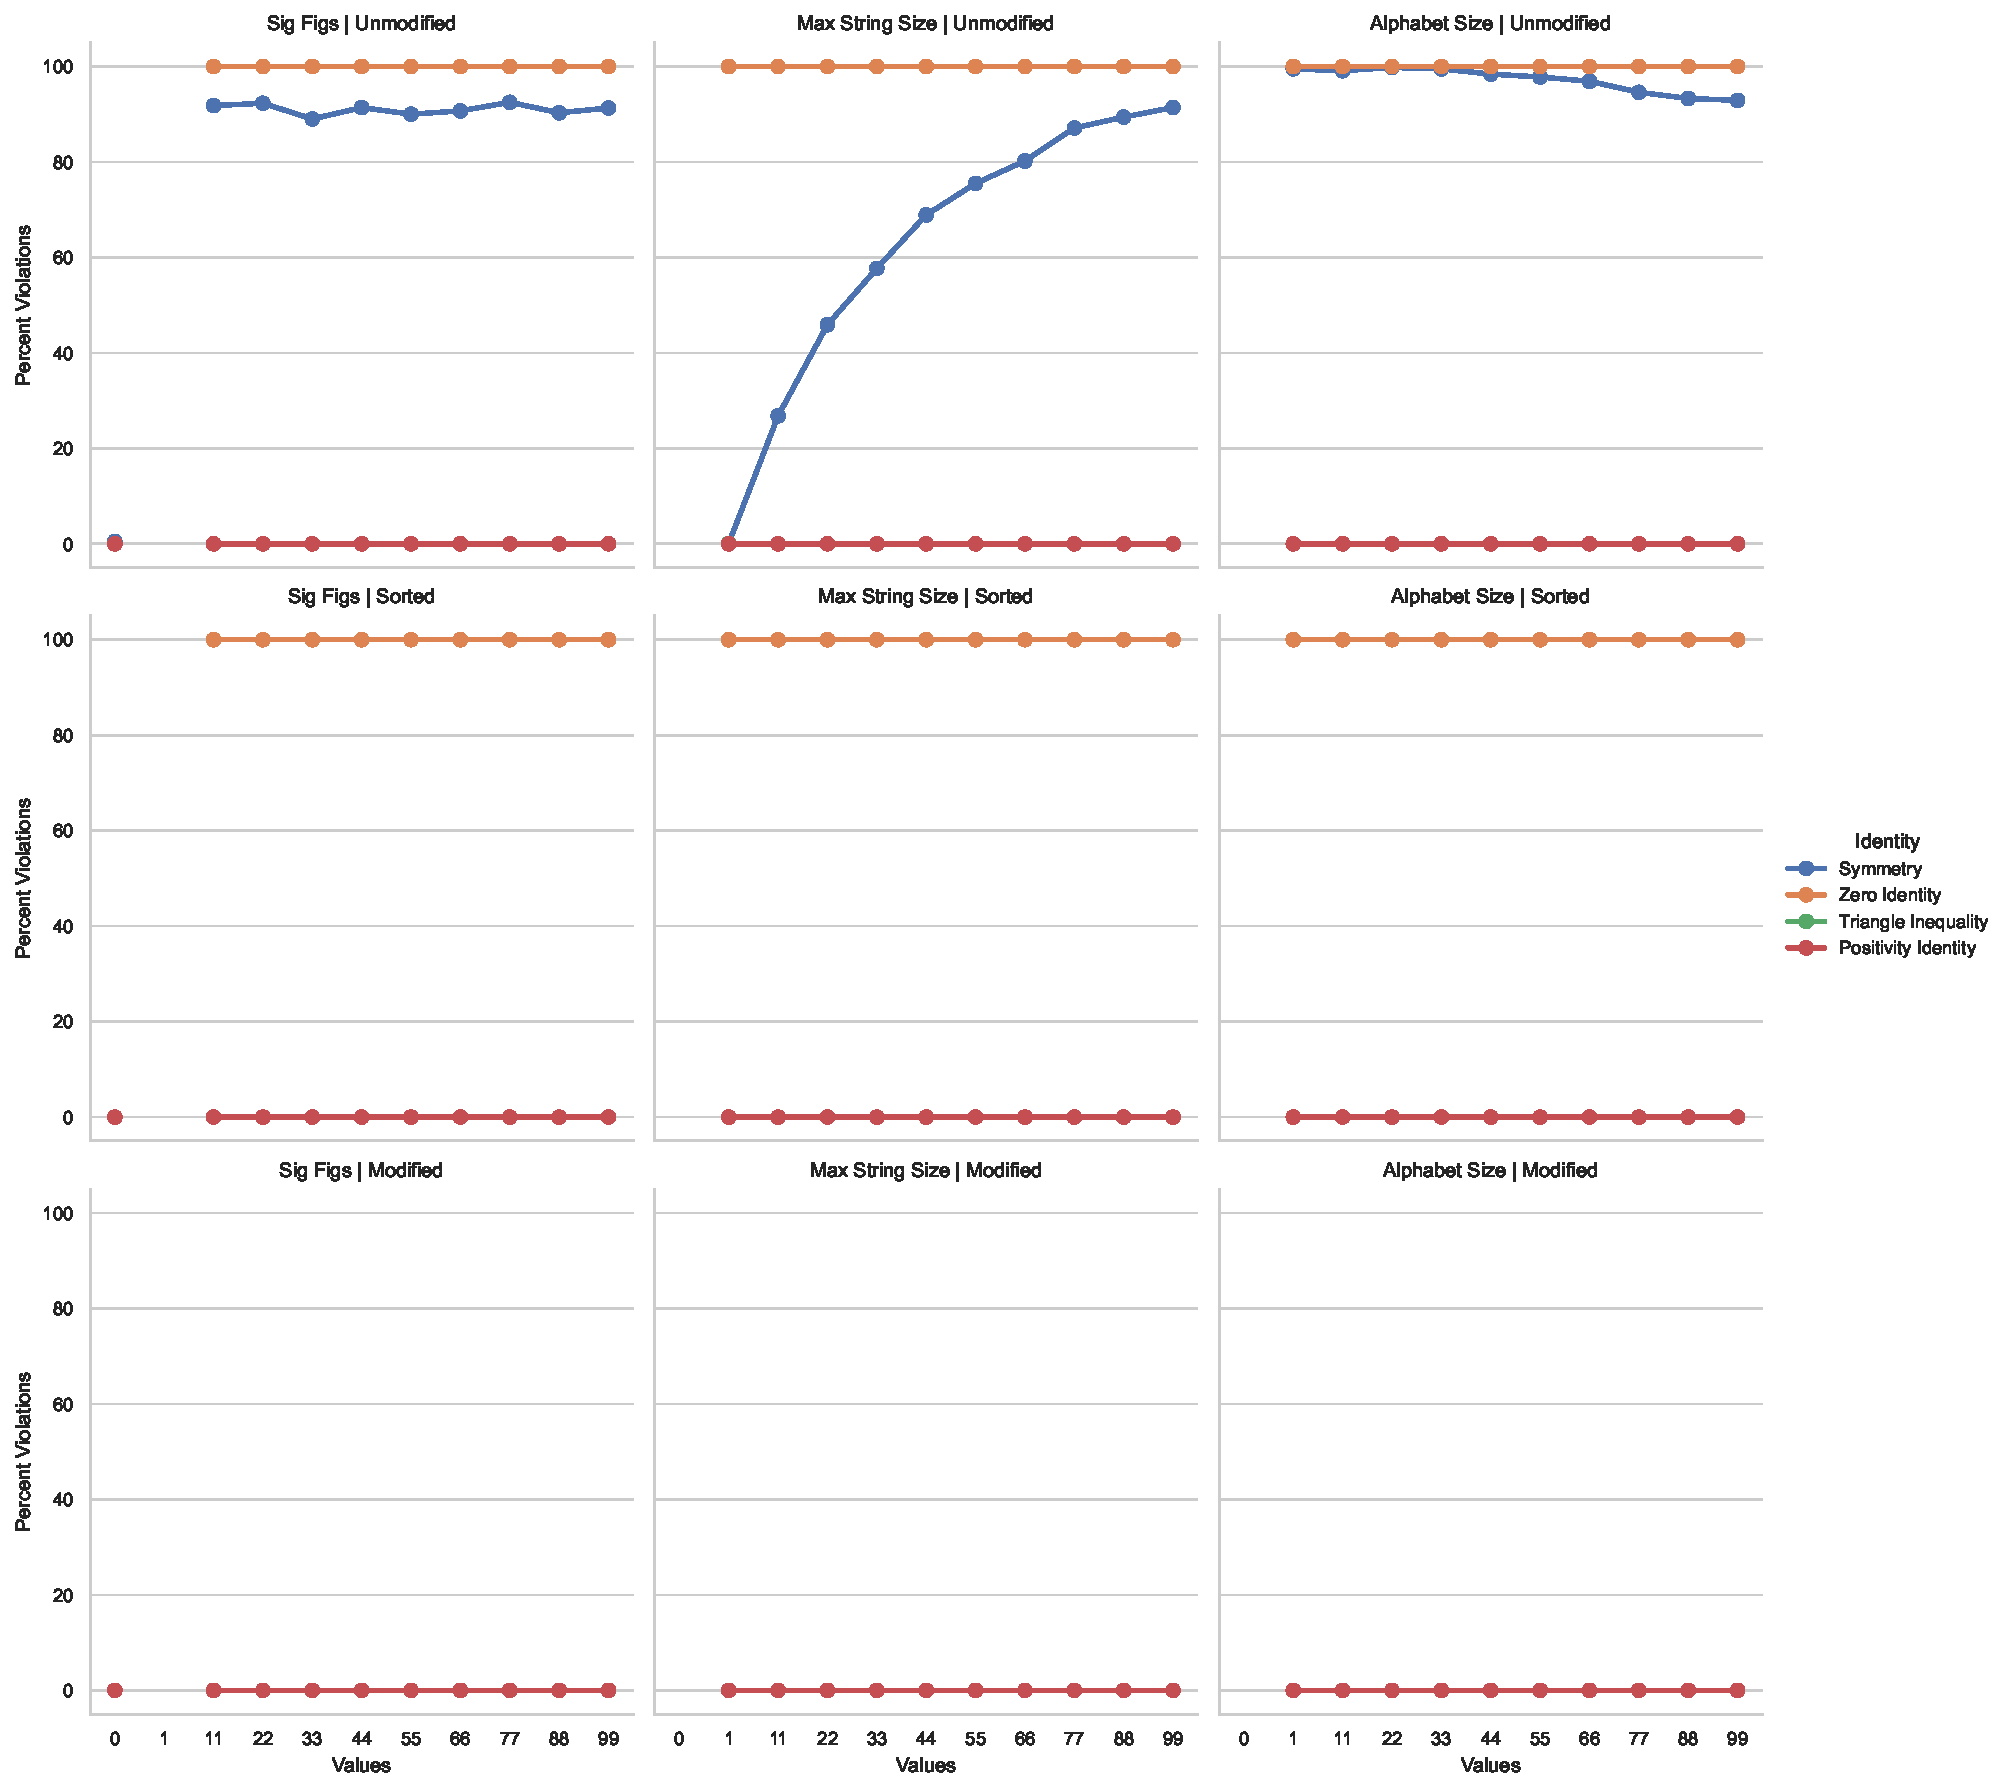
\includegraphics[width=\textwidth]{images/ncd.pdf}
    \caption{Percentage of examples found that violate the assumptions outlined in Section~\ref{metric_spaces} using the vanilla (Algorithm~\ref{alg:knn}), assumed-symmetry(Algorithm~\ref{alg:assumed_symmetry}), and enforced-symmetry (Algorithm~\ref{alg:enforced_symmetry}) algorithms and the \texttt{gzip} compression library on 100 thousand random strings. \textit{Sig Figs} refers to the number of significant figures. \textit{Max String Size} and \textit{Max Alphabet Size} refer to the number of characters and the number of unique characters respectively. Unless otherwise specified by the x-axis in an individual plot, \textit{Max String Size}, \textit{Max Alphabet Size}, and \textit{Significant Figures} were all 10. }
    \label{fig:mod_assumptions}

\end{figure*}

\begin{figure*}[htb]
    \centering
    \begin{subfigure}[htb]{\textwidth}
        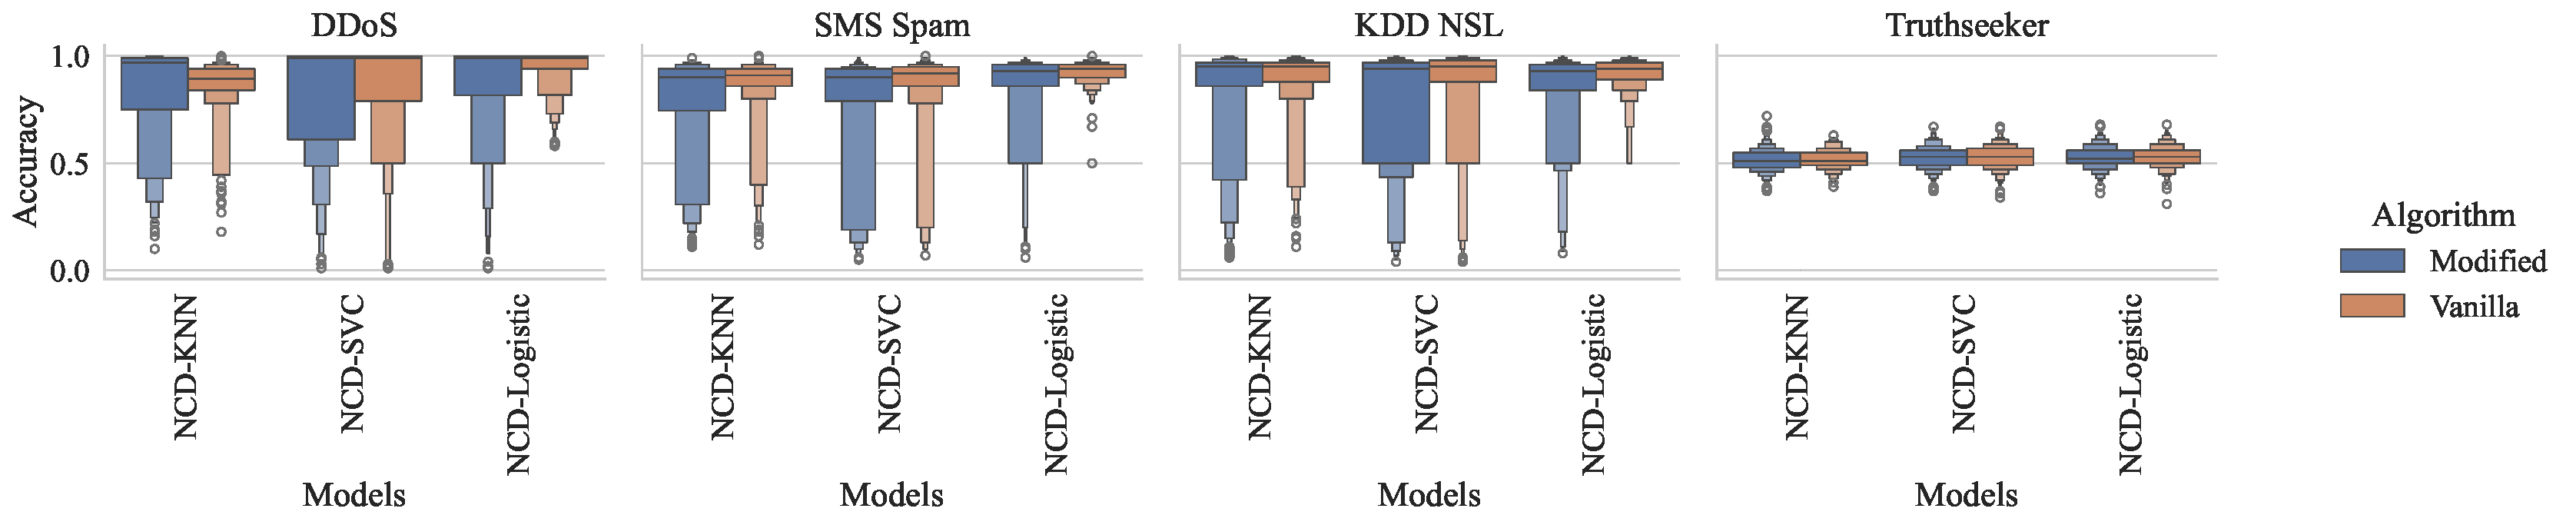
\includegraphics[width=\textwidth]{figs/combined/modified_models_vs_accuracy.pdf}
        \caption{Accuracy across models and datasets.}
        \label{fig:mod_acc}
    \end{subfigure}
    \begin{subfigure}[htb]{\textwidth}
        \centering
        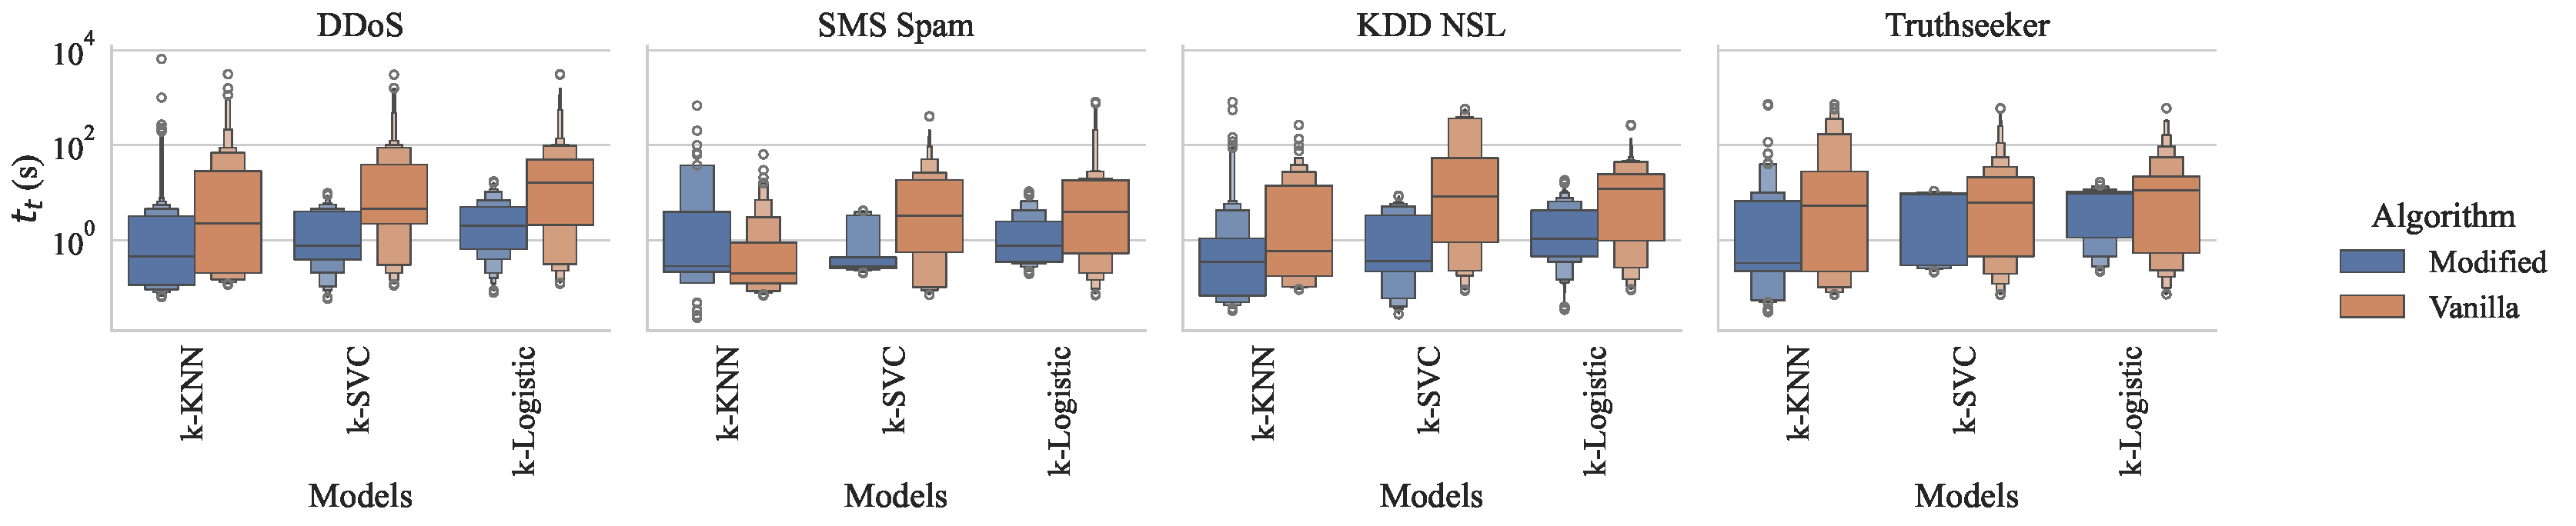
\includegraphics[width=\textwidth]{figs/combined/modified_models_vs_train_time.pdf}
        \caption{Training Times across models and datasets.}
        \label{fig:mod_train_time}
    \end{subfigure}
    \begin{subfigure}[htb]{\textwidth}
        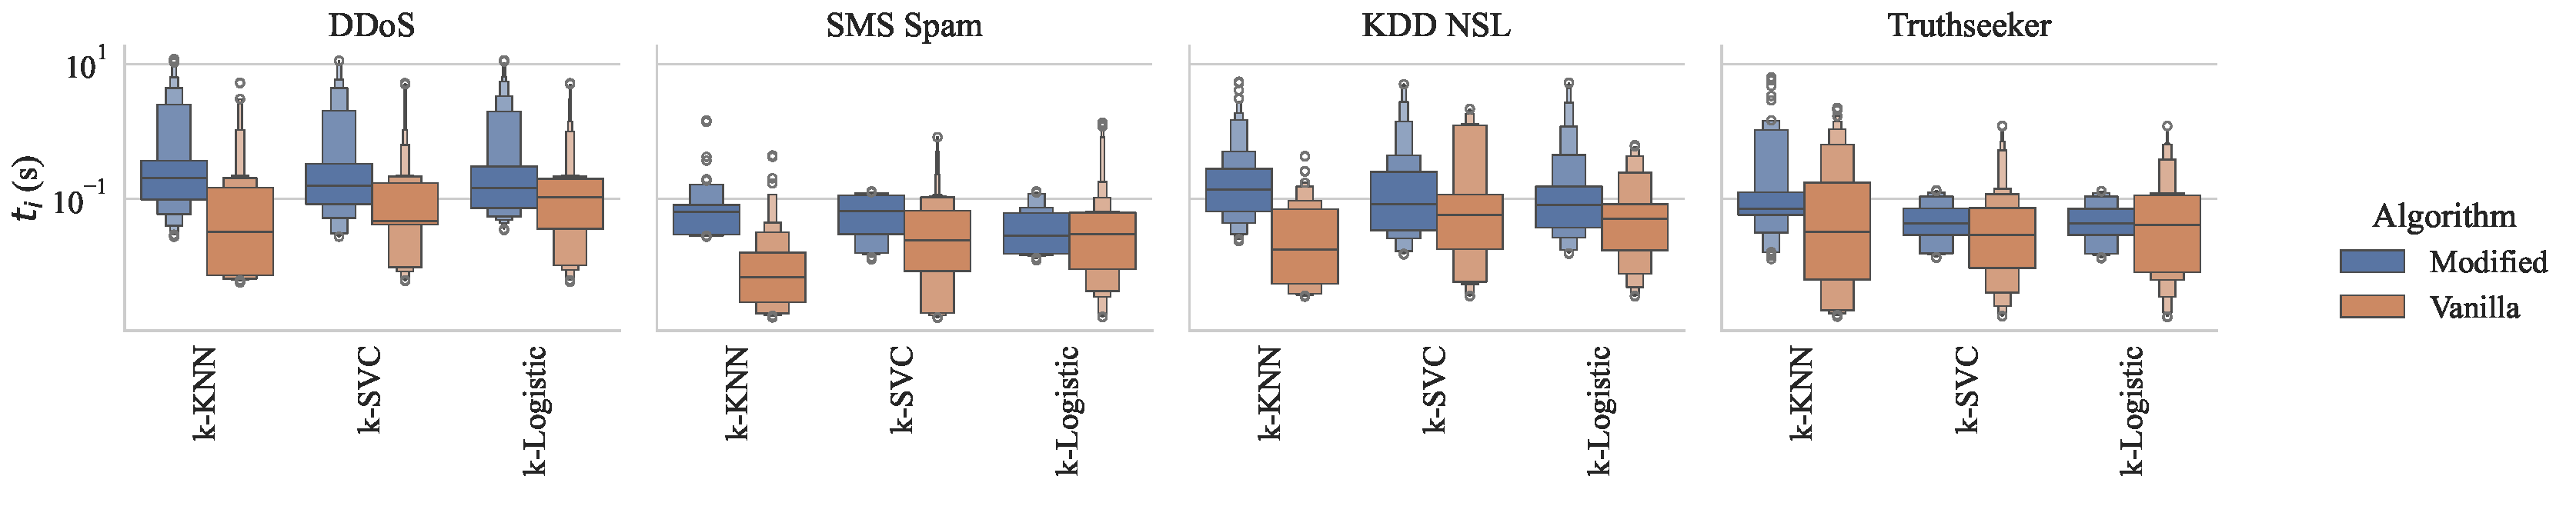
\includegraphics[width=\textwidth]{figs/combined/modified_models_vs_predict_time.pdf}
        \caption{Prediction Times across models and datasets.}
        \label{fig:mod_pred_time}
    \end{subfigure}
    \caption{Kernelized classifier inference times across many datasets, and models while examining the effect of the symmetric assumption outlined in Algorithm~\ref{alg:enforced_symmetry}. Each column corresponds to a different dataset and each row corresponds to a different performance metric, the value of which is on the y-axis. The x-axis in each plot corresponds to a classifier type and the colour conveys whether symmetry was assumed (orange) or not (blue).}
    \label{fig:mod_summary}
\end{figure*}

Figure~\ref{fig:mod_summary} depicts the accuracy (top), training time per sample (middle), and inference time per sample (bottom) for each the vanilla (denoted in orange) and the modified algorithm (see: Algorithm~\ref{alg:enforced_symmetry}, denoted in blue). As we can see, the accuracy of the modified algorithm is fairly consistent with the unmodified version. While there is a measured difference in the mean between the k-SVC on the DDoS dataset and k-KNN on the SMS Spam dataset, the extrema are the same and this difference in mean is likely due to inconsistent performance of the hyper-parameter optimisation algorithm rather than a true difference in performance~\cite{tpe}. In practice, the model builder would choose the most accurate model, which is consistent across the algorithms and classifiers for each dataset. However, we see that the modified version of the algorithm is much faster per sample when constructing the Gram matrix ($t_t$) by reducing the number of distance computations by a factor of 2. This comes at the marginal cost of a few hundred milliseconds for each prediction, however, but this could easily be mitigated by skipping the algorithmic modifications during the prediction step and handle the problem of negative distances at run-time, depending on the particular application. Overall, it is clear that this modified version of NCD offers significant run-time improvements while costing nothing in terms of accuracy. 
Additionally, by running the vanilla version during prediction and using the modified version if and only if the Gram matrix is calculated, these downsides can be avoided entirely. 
However, that may produce Gram matrices that are incompatible with other tooling or models (see: Figure~\ref{fig:mod_assumptions}, middle row), most of these are mitigated with the proposed modifications (see: Figure~\ref{fig:mod_assumptions}, bottom row). 
However, two classes of counterexamples remain. 
The first occurs with very short strings
$NCD("ABB", BBBB) =0$ because the marginal length associated with the repeated ``BB'' token happens to be the exact length as the marginal length associated with the token ``A''. 
This second occurs for the triangle inequality. 
Letting $x =AACAABC, y = AA,
z=AAA$, we find that $NCD(x,y) \approx .26$ while $NCD(x,z) + NCD(z,y) \approx .23$, but it's not clear that this is a problem in the theory. Including the string ``AAA'' provides additional context that ``AA'' may have a distinct meaning apart from ``A'' repeated twice which is why the distance of the sum \textit{is} less than the distance between $x$ and $z$. Additionally, it doesn't seem to be a problem in practice. As the max string size or the maximum alphabet size is increased, these problems quickly disappear(see: Figures~\ref{fig:mod_assumptions}~and~\ref{fig:mod_acc}).




\subsection{Database Condensing Methods}

\begin{figure*}[htb]
    \centering
    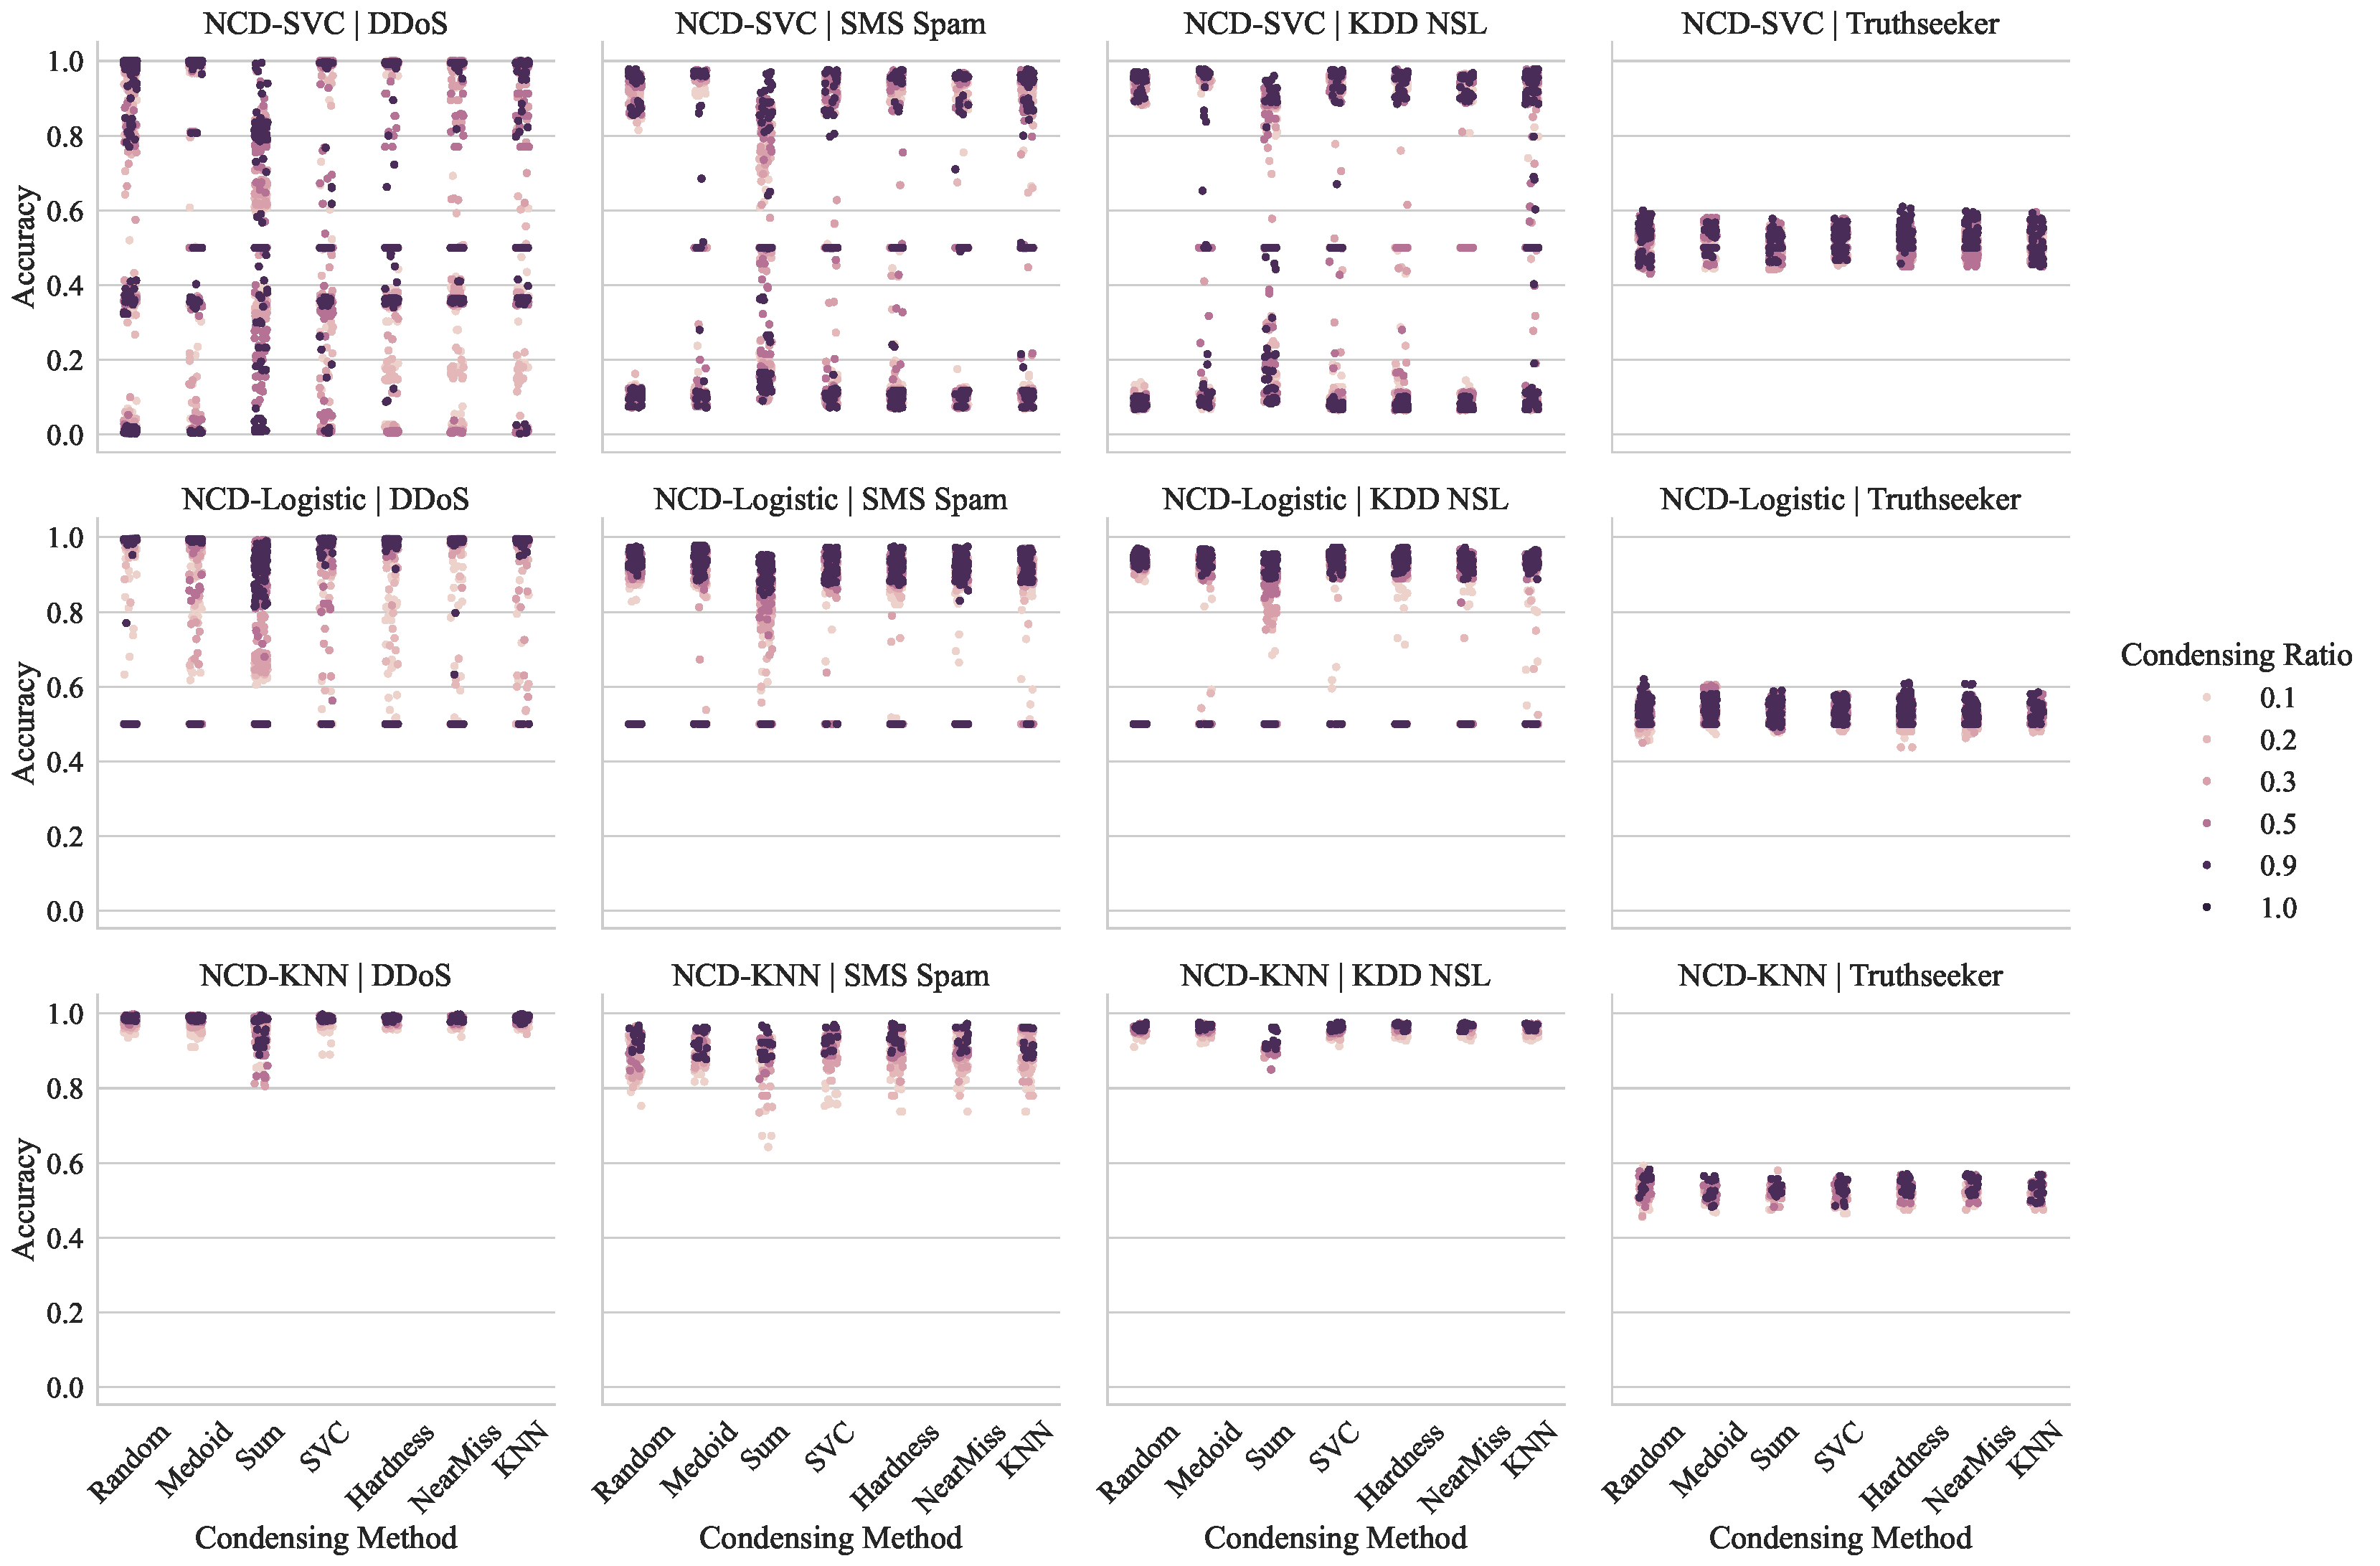
\includegraphics[width=\textwidth]{figs/combined/condensing_ratio_vs_accuracy.pdf}
    \caption{Accuracy across models (rows) and datasets (columns) where the hue represents the condensing ratio. }
    \label{fig:condense_acc_ratios}
\end{figure*}

\begin{figure*}[htb]
    \begin{subfigure}[htb]{\textwidth}
        \centering
        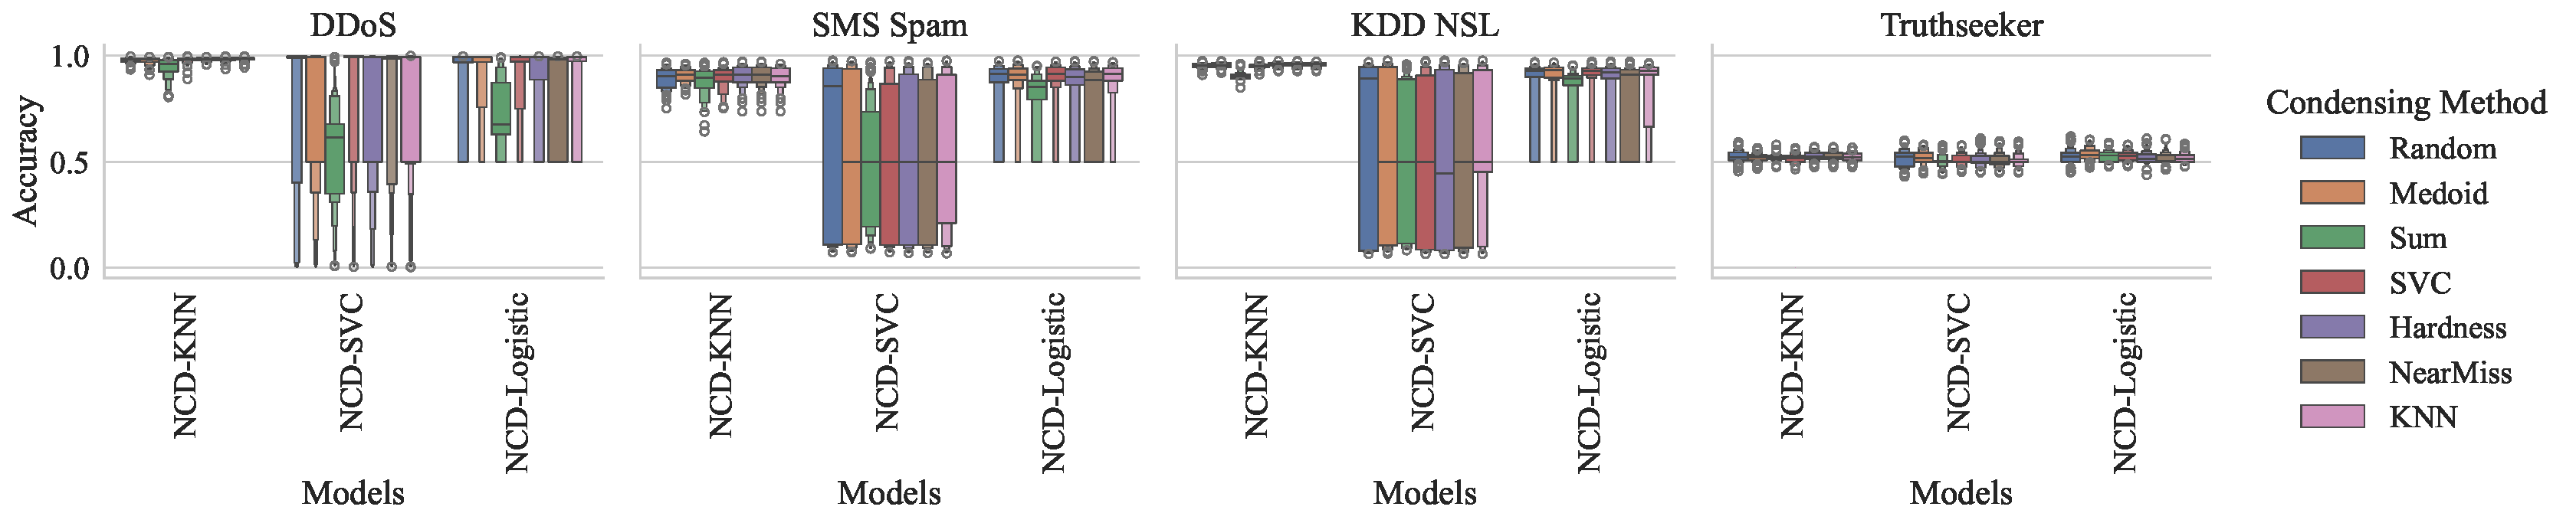
\includegraphics[width=\textwidth]{figs/combined/condensing_methods_vs_accuracy.pdf}
        \caption{Training Times across models and datasets.}
        \label{fig:condense_acc}
    \end{subfigure}
    \begin{subfigure}[htb]{\textwidth}
        \centering
        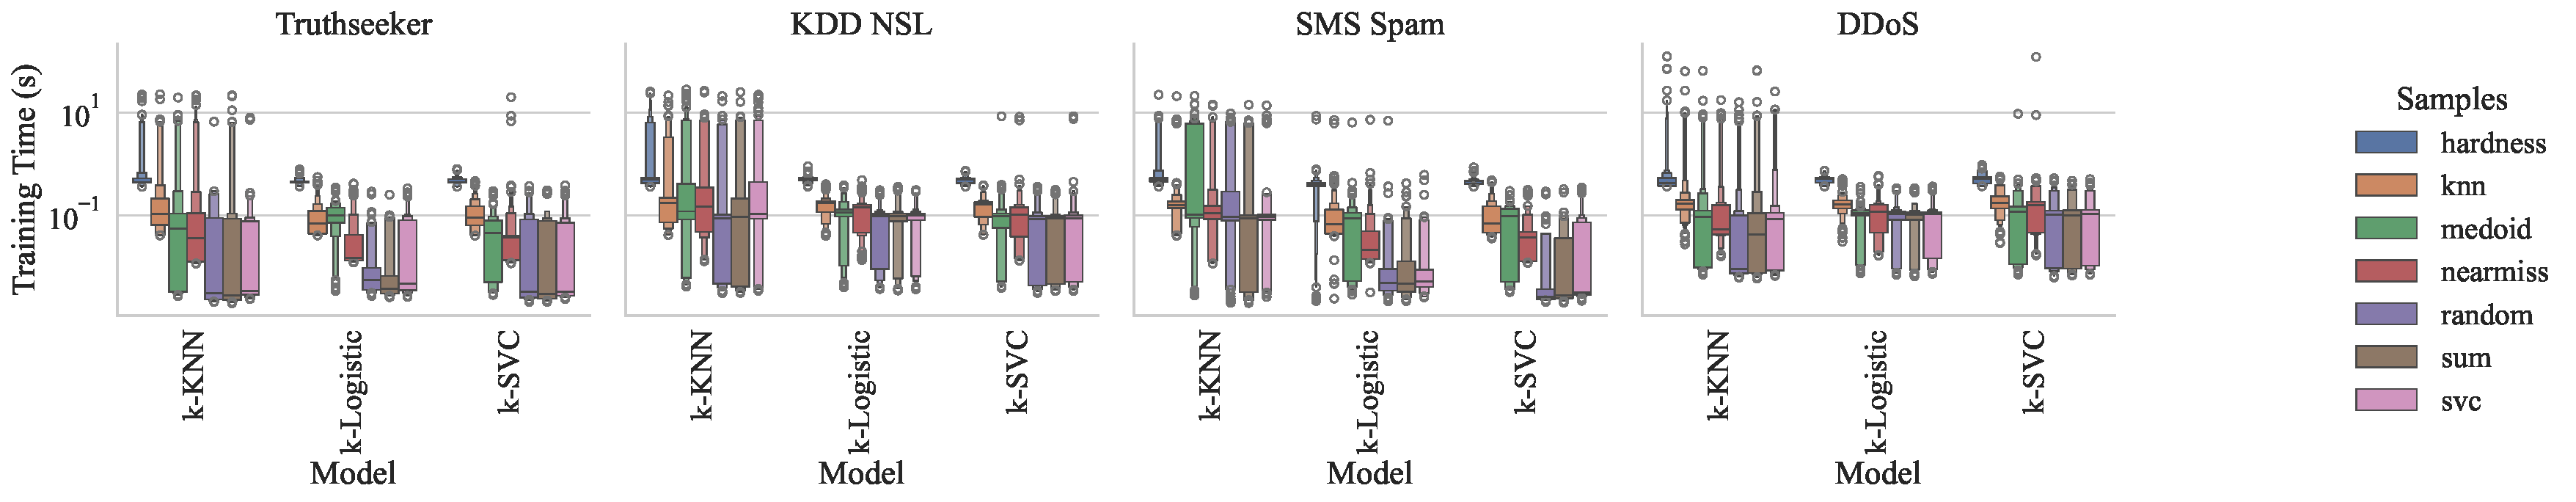
\includegraphics[width=\textwidth]{figs/combined/condensing_methods_vs_train_time.pdf}
        \caption{Training Times across models and datasets.}
        \label{fig:condense_train_time}
    \end{subfigure}
    \begin{subfigure}[htb]{\textwidth}
        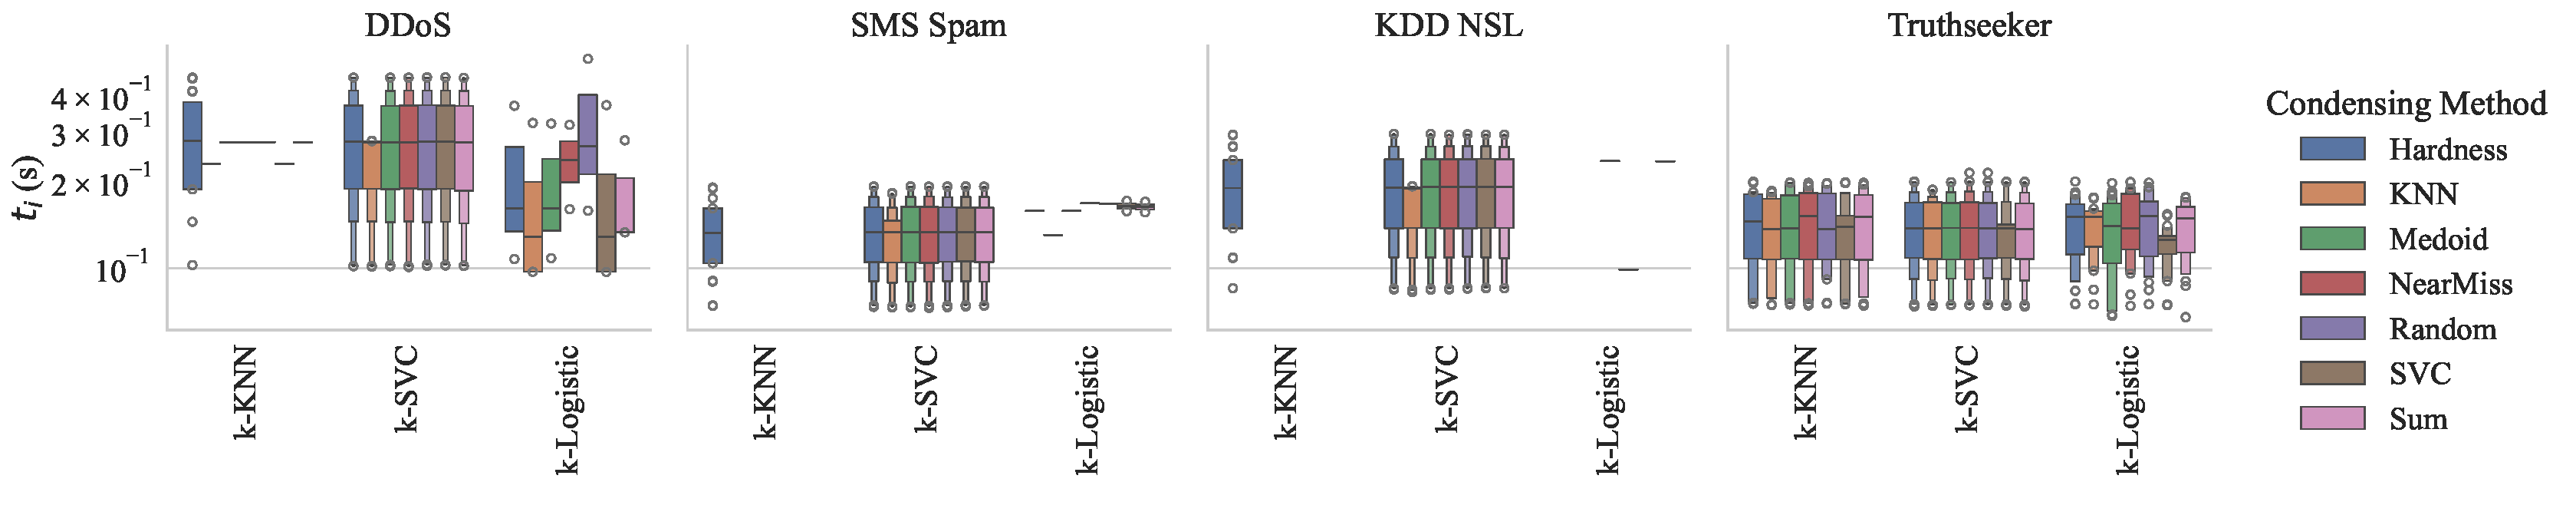
\includegraphics[width=\textwidth]{figs/combined/condensing_methods_vs_predict_time.pdf}
        \caption{Prediction Times across models and datasets.}
        \label{fig:condense_pred_time}
    \end{subfigure}
    \caption{Kernelized classifier inference times across many datasets, and models while examining the effect of the symmetric assumption outlined in Algorithm~\ref{alg:enforced_symmetry}. Each column corresponds to a different dataset and each row corresponds to a different performance metric, the value of which is on the y-axis. The x-axis in each plot corresponds to a classifier type and the colour conveys whether symmetry was assumed (orange) or not (blue).}
    \label{fig:condense_summary}
\end{figure*}

Figure~\ref{fig:condense_acc_ratios} depicts the accuracy across all models, datasets, and condensing ratios while Figure~\ref{fig:condense_summary} depicts the run-time requirements of various condensing methods. 
For each test, 1000 training samples were used to calculate the Gram matrix. 
Then, 400 test samples were used to calculate the accuracy across 10 random splits of the data. 
For each condensing ratio (e.g. percentage of training samples used during prediction), 128 trials were conducted to tune the hyper-parameters of each of the tested models using a variety of methods (see: Section~\ref{condensing_methods} and Figure~\ref{fig:condense_summary}). 
) However, the run-time improvements are obvious since the distributions of training times and inference times ($t_t, t_t$ respectively) is effectively the same in both Figures~\ref{fig:condense_summary} and \ref{fig:mod_summary}. That is the condensing methods themselves are fast enough to more than overcome their run-time downsides. However, while it is clear from the former that NCD is quite capable of performing very well on even a small number of samples since the distribution in accuracy does not seem to rely on the compression ratio (see: Figure~\ref{fig:condense_acc_ratios}) and that none of the tested condensing methods consistently outperforms random chance (see: Figure~\ref{fig:condense_acc} meaning this stage is probably unnecessary in practice and that any random subset of samples will be ``good enough''. 

% \begin{figure*}
%      \centering
%     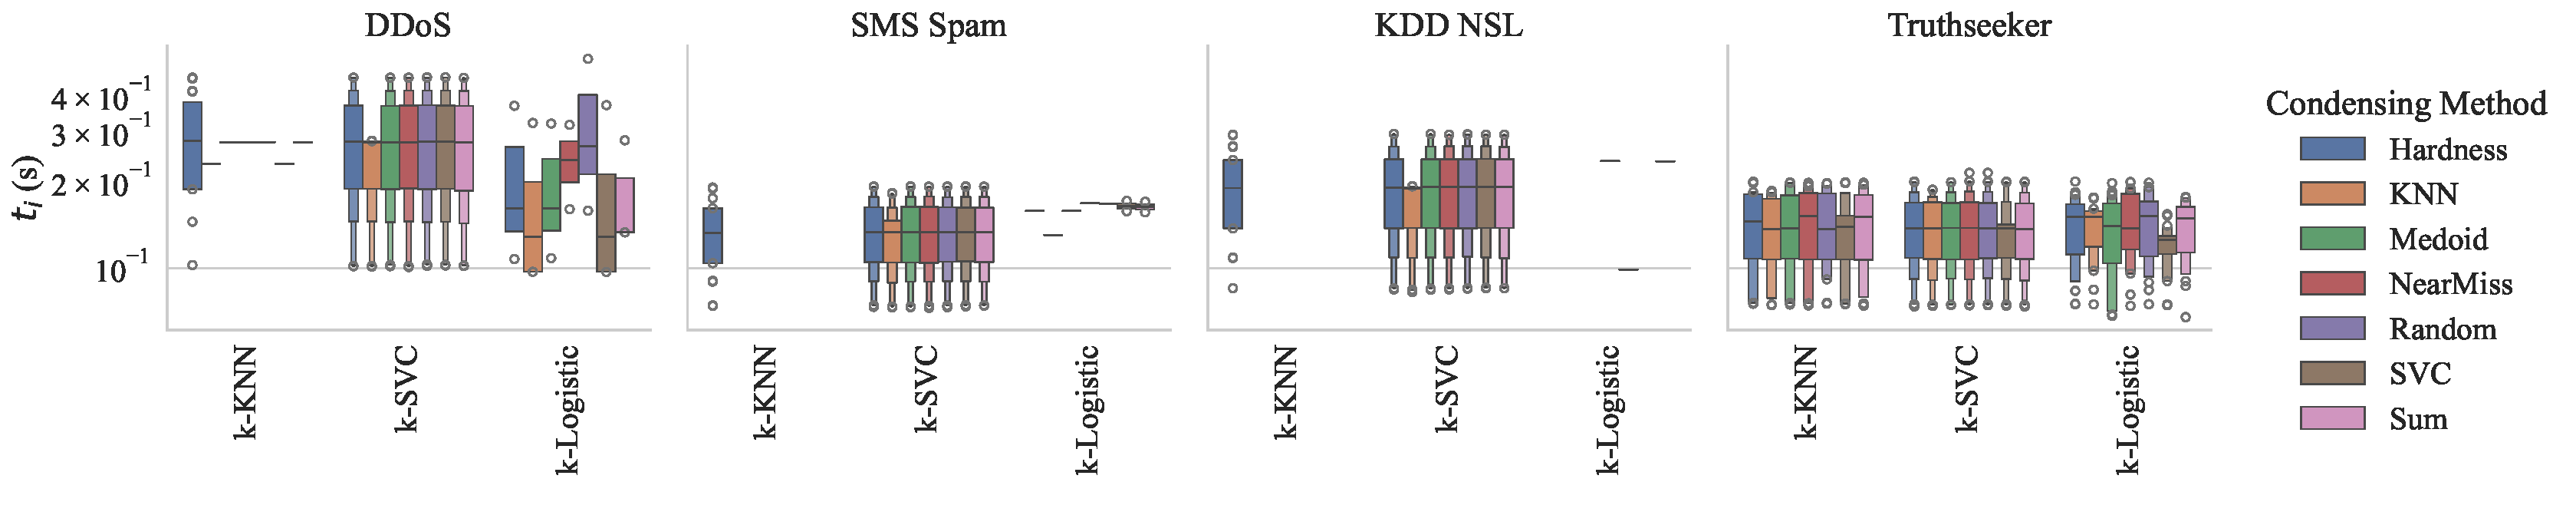
\includegraphics[width=\textwidth]{figs/combined/condensing_methods_vs_predict_time.pdf}
%     \caption{Kernelized classifier inference times across many datasets, models, while examining the effect of different condensing techniques (see Algorithm~\ref{alg:condensing}). Each column corresponds to a different dataset and each row corresponds to a different performance metric, the value of which is on the y-axis. The x-axis in each plot corresponds to a classifier type and the colour conveys whether symmetry was assumed (orange) or not (blue).}
%     \label{fig:cond_pred_time}
% \end{figure*}


\section{Considerations}
\label{considerations}
While the proposed algorithm (see:~\ref{alg:enforced_symmetry}) does improve upon certain edge cases outlined in Section~\ref{pseudometric}, the examined condensing methods (see: Section~\ref{condensing}) do not improve upon models trained on samples selected by random chance (see:~\ref{fig:condense_acc}). However, the resulting lack of negative distances allows NCD to be used as part of a kernelized classifier (see: Figures~\ref{fig:condense_acc}~and~~\ref{fig:condense_acc_ratios} to great effect. 
By assuming and enforcing symmetry using the method outlined in Algorithm~\ref{alg:enforced_symmetry}, the training step can be significantly improved.
However, the vanilla NCD-KNN proposed by Jiang et. al.~\cite{jiang2022less} remains an effective choice if the training step is deemed too expensive for the chosen applications.
Here, the authors would like to note the borderline performance of all metrics on the Truthseeker dataset--- both NCD and more traditional distance measures. However, this is on par with the performance from the original authors~\cite{truthseeker}. To the best knowledge of the authors, most content on the platform formerly known as Twitter is simply indistinguishable from bot-generated spam--- using any known distance metric.


\section{Conclusion}
It is clear from Figure~\ref{fig:mod_summary} that our algorithm is superior to the method proposed by Jiang et. al. when applied used a distance measure for kernelized classifiers. By preemptively handling cases that would result in negative values for distance (thus violating the Non-negativity identity) and sorting the inputs, this modified NCD is guaranteed to behave more like a true metric. 
This allows the model builder to use standard tooling (e.g.~\texttt{scikit-learn},~\texttt{imblearn}) to build classifiers that perform well on an exceedingly small number of samples. The end result is a real-time, client-side classification algorithm that doesn't rely on federation, centralization, or the large scale processing of millions of data points across a global user-base. 
This categorically circumvents poisoning attacks~\cite{biggio_poisoning_2013} since each labelled database is unique to each user. 
Furthermore, this reduces the attack surface of attacks like model inference attacks, database exfiltration attacks, and evasion attacks since a malicious user would need to target the personalised classifier of each user~\cite{biggio_evasion_2013,deepfool,chakraborty_adversarial_2018}. 
While it is known that some attacks are quite transferable~\cite{wang2021enhancing}, this reduces the common attack surface to \textit{only} the samples that are universal across the user base and a new model can be generated trivially by refreshing the page or appending the offending sample to the labelled (training) dataset. 


\label{conclusion}


\bibliographystyle{ieeetr}
\newpage
\bibliography{bibliography}

% \clearpage
% \appendix
% \onecolumn
% \subsection{DDoS}
This subsection reveals more granular data about the DDoS dataset.

\subsubsection{Accuracy}
Figure~\ref{fig:ddos_accuracy} shows the accuracy of different compressors, metrics, and sample selection methods.

\begin{figure}[h!]
	\centering
    \captionsetup[subfigure]{skip=0pt}
	\begin{subfigure}[t]{.44\textwidth}
		\centering
		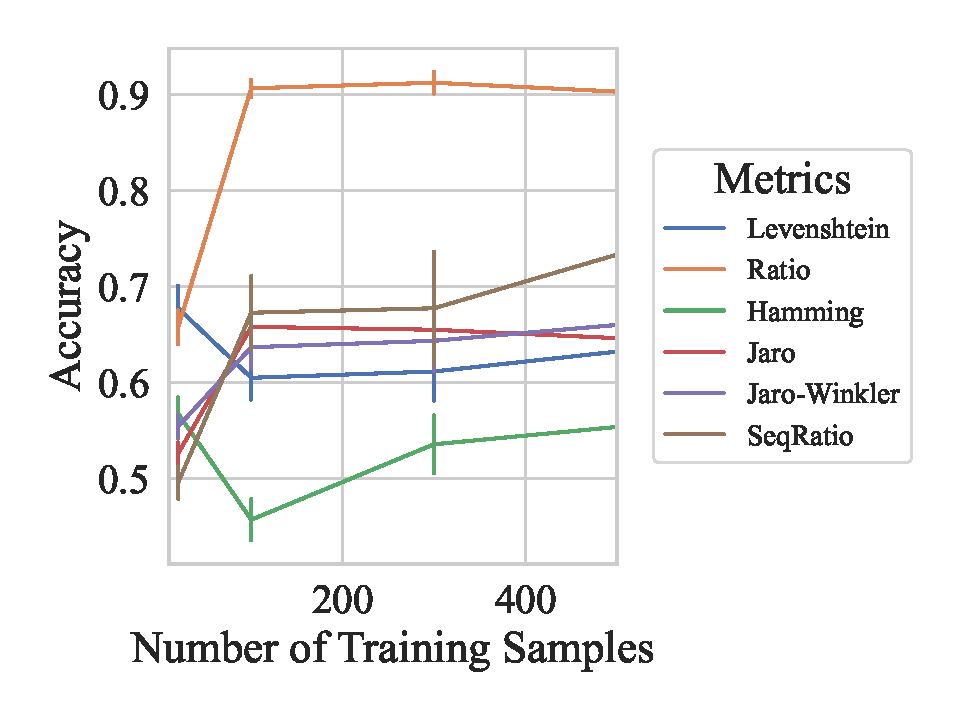
\includegraphics[width=\textwidth]{figs/ddos/string_metric_vs_accuracy.pdf}
	\end{subfigure}
	~
	\begin{subfigure}[t]{.44\textwidth}
		\centering
		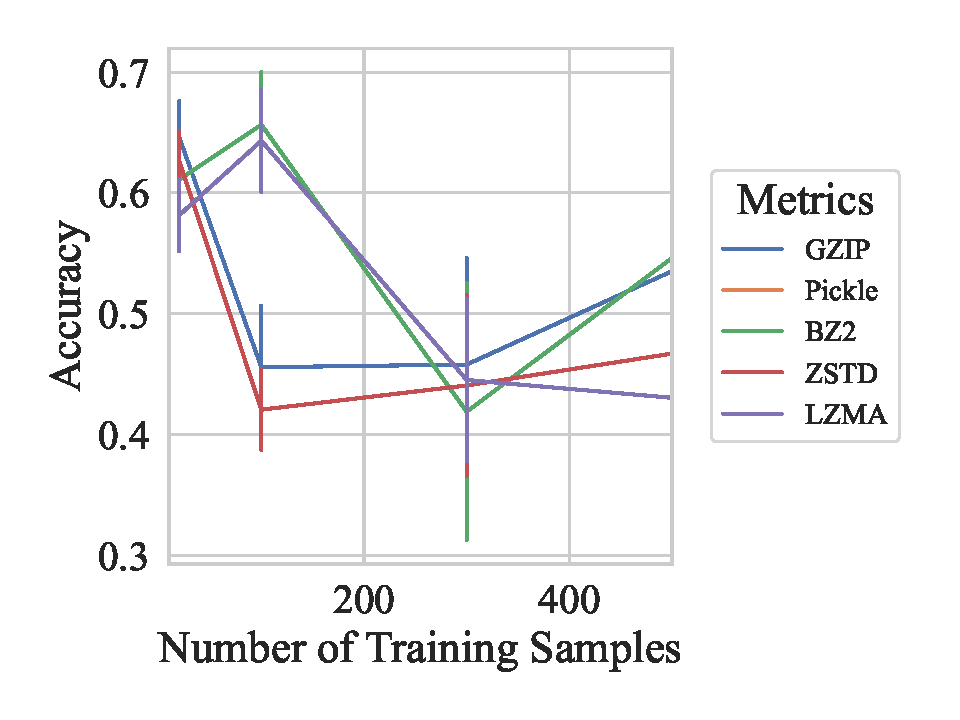
\includegraphics[width=\textwidth]{figs/ddos/compressor_metric_vs_accuracy.pdf}
	\end{subfigure}
	\caption{Accuracy across different different string kernel metrics (left), and compression methods (right).}
	\label{fig:ddos_accuracy}
\end{figure}

\subsubsection{Training Time}

Figure~\ref{fig:ddos_training_time} depicts the training time across all the tested compressors, distance metrics, and sample selection methods.

\begin{figure}[h!]
    \centering
    \captionsetup[subfigure]{skip=0pt}
	\begin{subfigure}[t]{.44\textwidth}
		\centering
		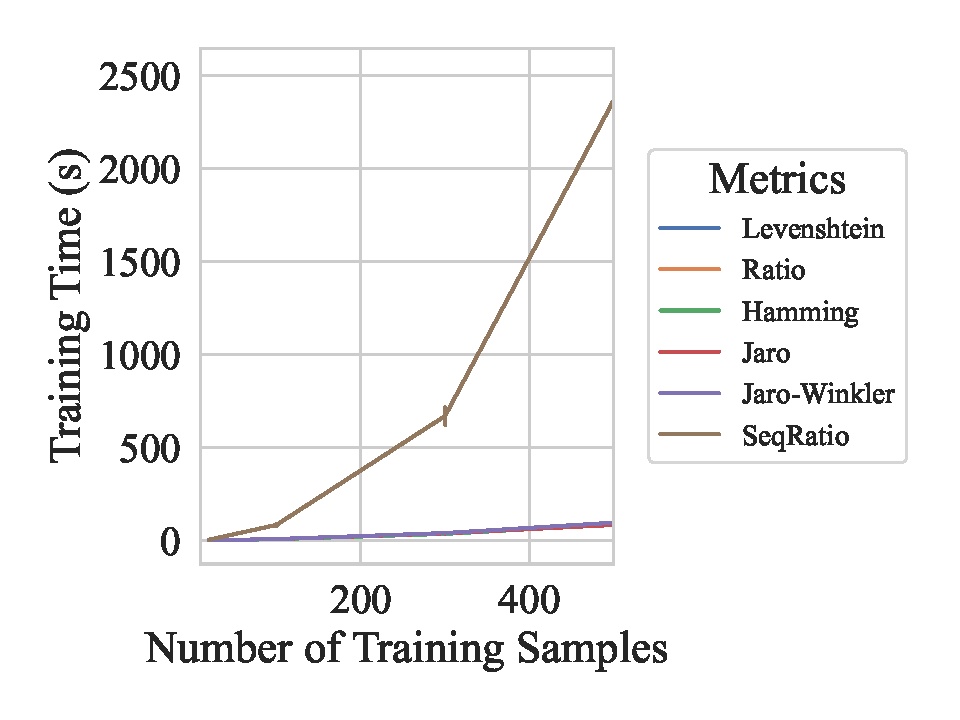
\includegraphics[width=\textwidth]{figs/ddos/string_metric_vs_train_time.pdf}
	\end{subfigure}
	~
	\begin{subfigure}[t]{.44\textwidth}
		\centering
		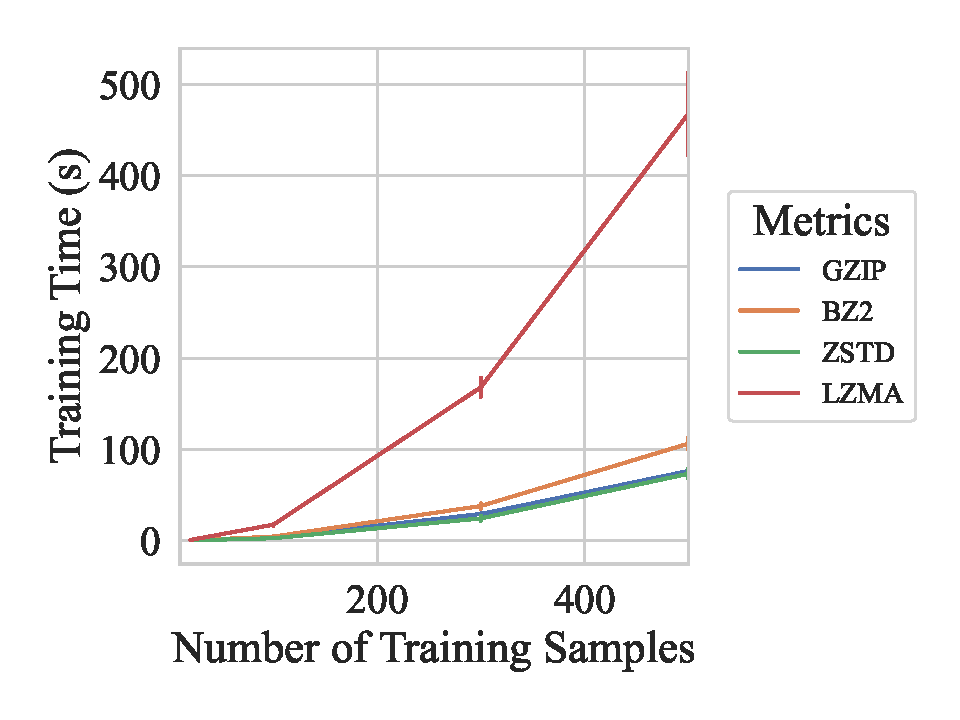
\includegraphics[width=\textwidth]{figs/ddos/compressor_metric_vs_train_time.pdf}
	\end{subfigure}
	\caption{Training time across different different string  metrics (left), and compression methods (right).}
	\label{fig:ddos_training_time}
\end{figure}

\subsubsection{Prediction Time}

Figure~\ref{fig:ddos_prediction_time} shows the prediction time of different compressors, metics, and sample selection methods.
\begin{figure}[h!]
	\centering
    \captionsetup[subfigure]{skip=0pt}
	\begin{subfigure}[t]{.44\textwidth}
		\centering
		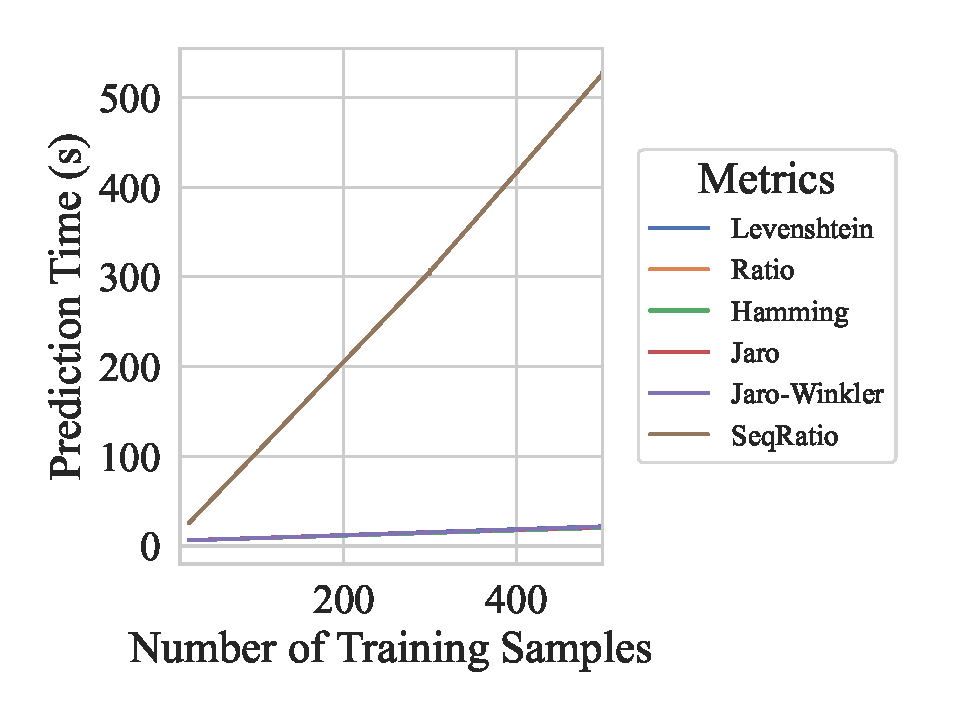
\includegraphics[width=\textwidth]{figs/ddos/string_metric_vs_predict_time.pdf}
	\end{subfigure}
	~
	\begin{subfigure}[t]{.44\textwidth}
		\centering
		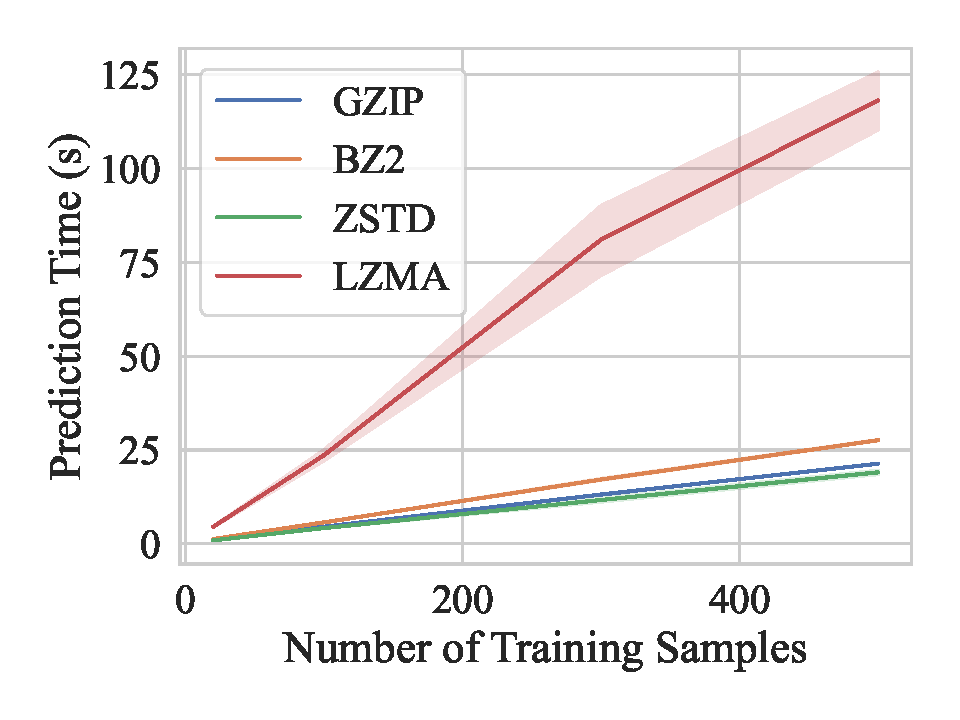
\includegraphics[width=\textwidth]{figs/ddos/compressor_metric_vs_predict_time.pdf}
	\end{subfigure}
	\caption{Prediction time across different different string metrics (left), and compression methods (right).}.
	\label{fig:ddos_prediction_time}
 
\end{figure}

\subsubsection{Symmetry}

Figure~\ref{fig:ddos_symmetry} shows the effect of assuming symmetry for different models and distance metrics.

\begin{figure}[h!]
    \centering
    \captionsetup[subfigure]{skip=0pt}
    \begin{subfigure}[t]{.44\textwidth}
        \centering
        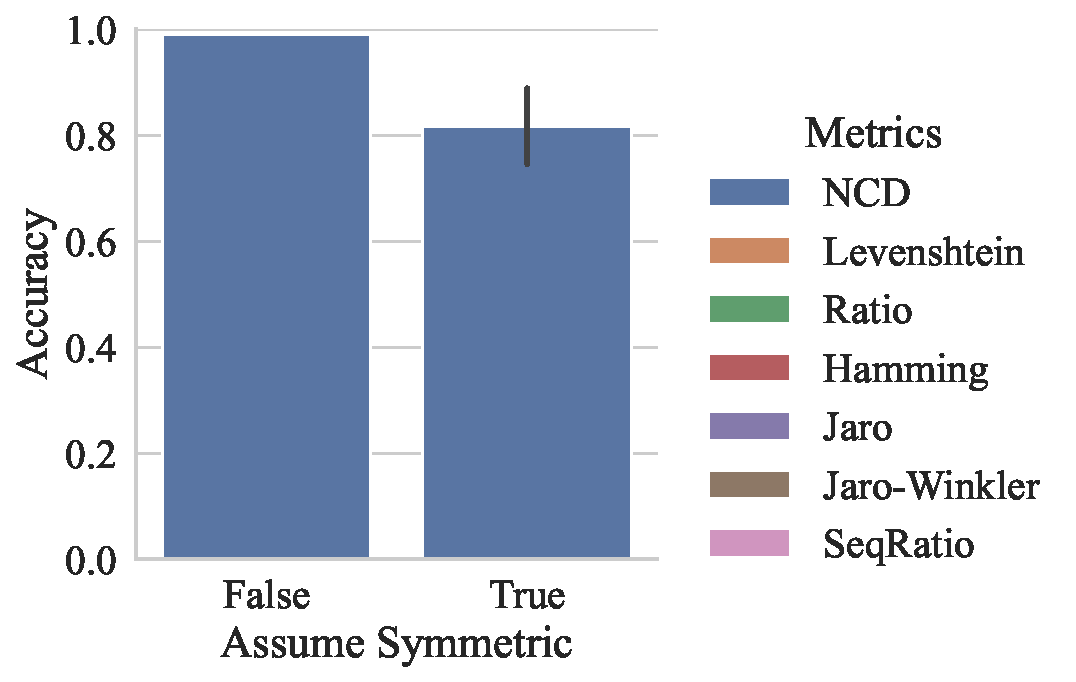
\includegraphics[width=\textwidth]{figs/ddos/symmetric_vs_metric.pdf}
    \end{subfigure}
    \begin{subfigure}[t]{.44\textwidth}
        \centering
        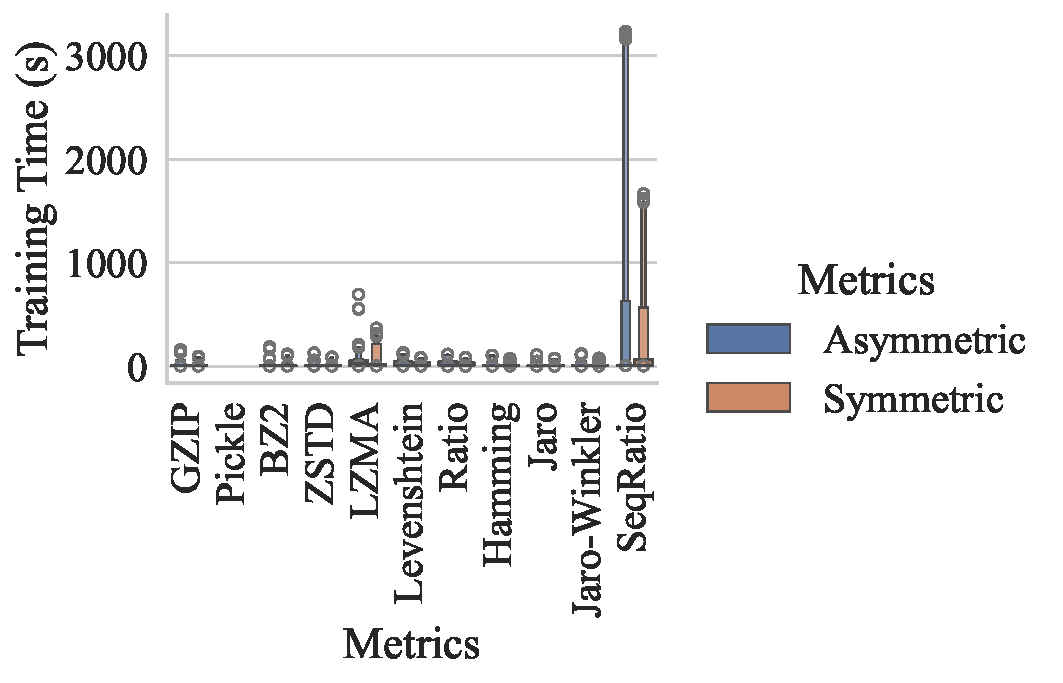
\includegraphics[width=\textwidth]{figs/ddos/symmetric_vs_metric_train_time.pdf}
    \end{subfigure}
    \caption{Accuracy across (left) and prediction time (right) across several compression methods and distance metrics with and without assuming symmetric distances.}
    \label{fig:ddos_symmetry}
\end{figure}
% \clearpage
% \subsection{SMS Spam}
This subsection reveals more granular data about the SMS Spam dataset.

\subsubsection{Accuracy}
Figure~\ref{fig:sms_spam_accuracy} shows the accuracy of different compressors, metrics, and sample selection methods.

\begin{figure}[h!][h]
	\centering
    \captionsetup[subfigure]{skip=0pt}
	\begin{subfigure}[t]{.44\textwidth}
		\centering
		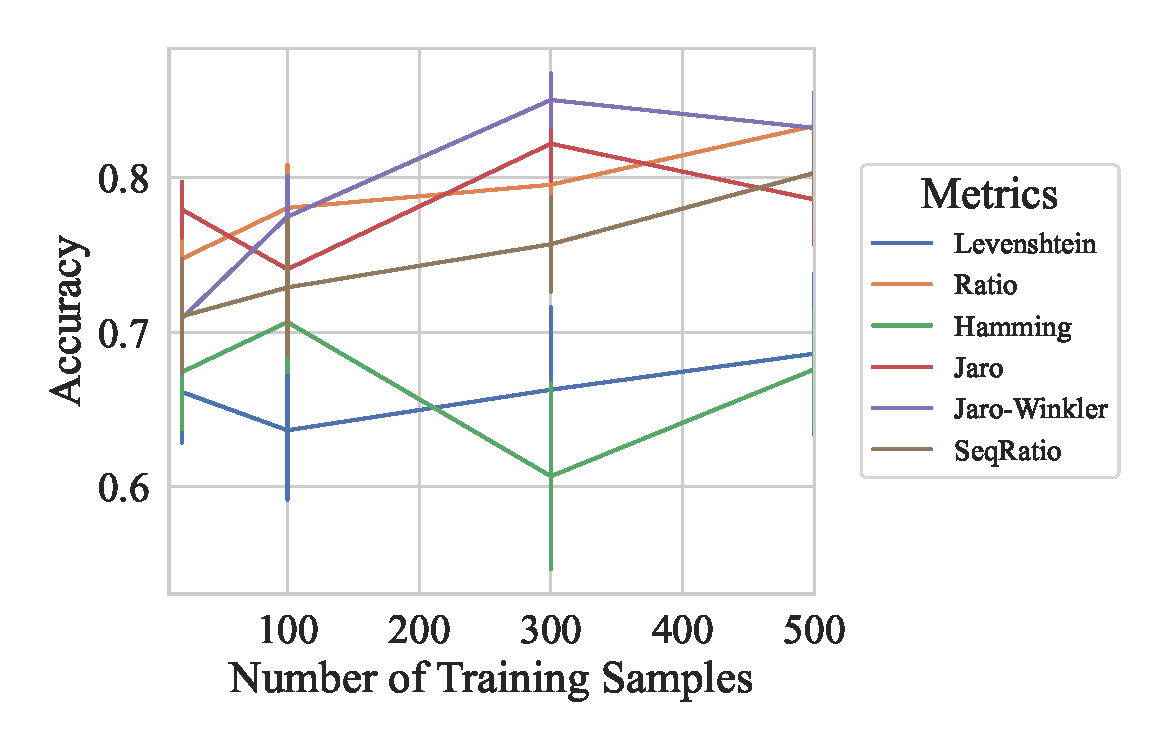
\includegraphics[width=\textwidth]{figs/sms_spam/string_metric_vs_accuracy.pdf}
	\end{subfigure}
	~
	\begin{subfigure}[t]{.44\textwidth}
		\centering
		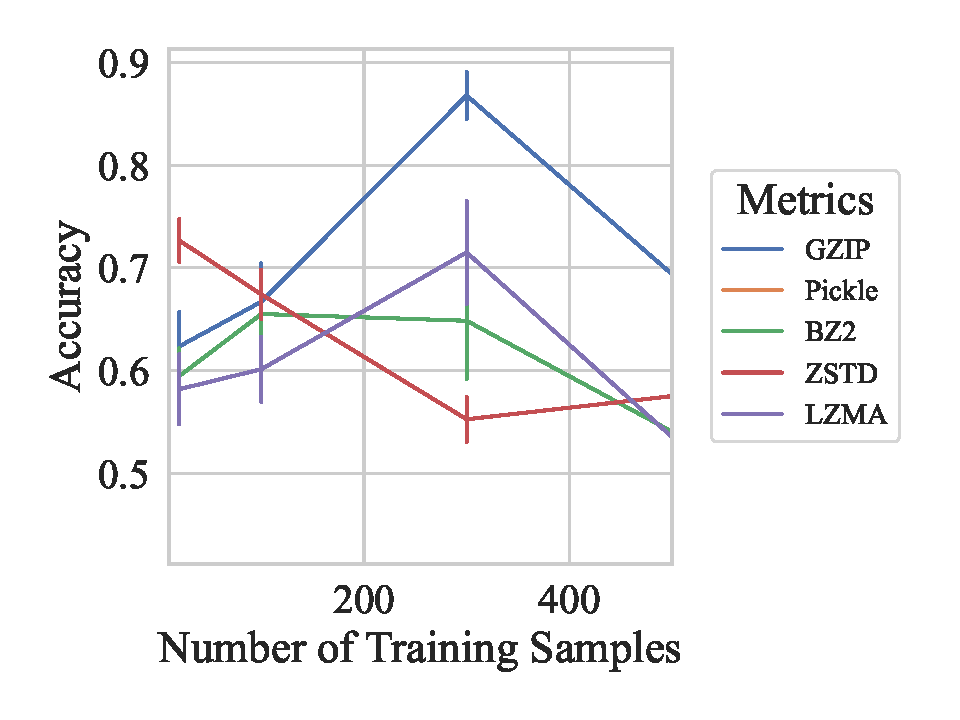
\includegraphics[width=\textwidth]{figs/sms_spam/compressor_metric_vs_accuracy.pdf}
	\end{subfigure}
	\caption{Accuracy across different different string kernel metrics (left), and compression methods (right).}
	\label{fig:sms_spam_accuracy}
\end{figure}

\subsubsection{Training Time}

Figure~\ref{fig:sms_spam_training_time} depicts the training time across all the tested compressors, distance metrics, and sample selection methods.

\begin{figure}[h!]
    \centering
    \captionsetup[subfigure]{skip=0pt}
	\begin{subfigure}[t]{.44\textwidth}
		\centering
		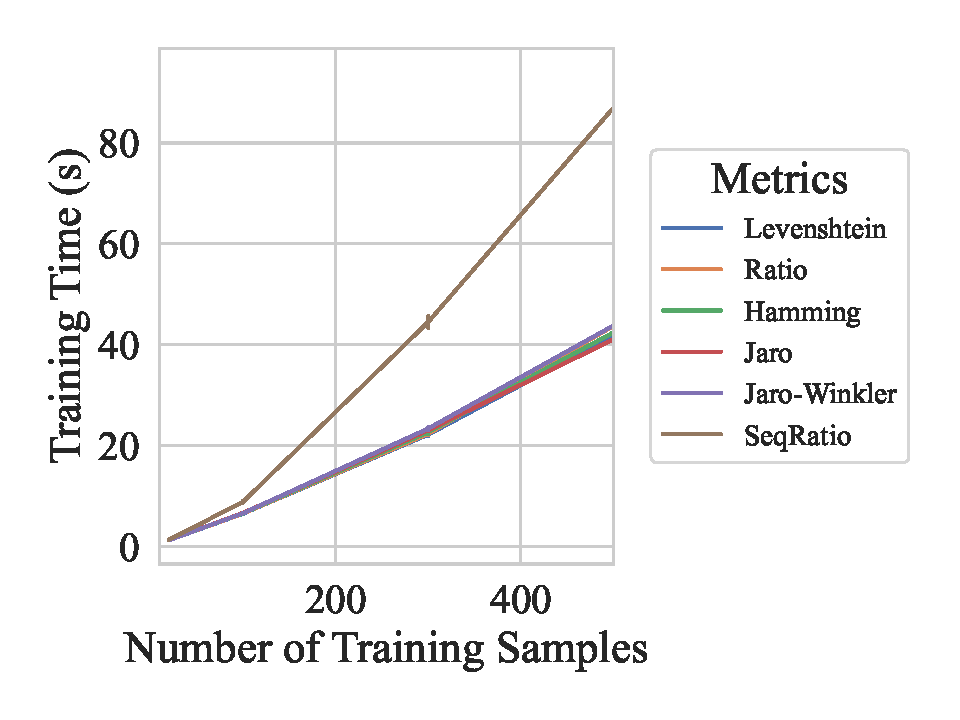
\includegraphics[width=\textwidth]{figs/sms_spam/string_metric_vs_train_time.pdf}
	\end{subfigure}
	~
	\begin{subfigure}[t]{.44\textwidth}
		\centering
		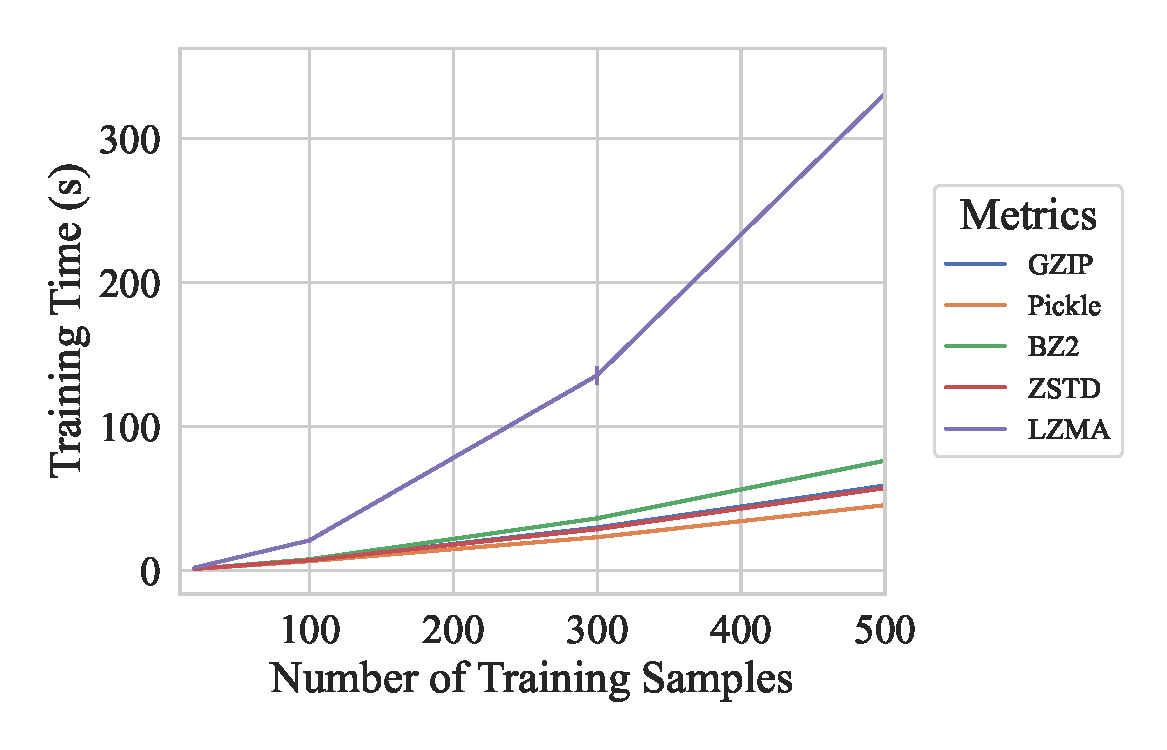
\includegraphics[width=\textwidth]{figs/sms_spam/compressor_metric_vs_train_time.pdf}
	\end{subfigure}
	\caption{Training time across different different string  metrics (left), and compression methods (right).}
	\label{fig:sms_spam_training_time}
\end{figure}

\subsubsection{Prediction Time}

Figure~\ref{fig:sms_spam_prediction_time} shows the prediction time of different compressors, metics, and sample selection methods.
\begin{figure}[h!]
	\centering
    \captionsetup[subfigure]{skip=0pt}
	\begin{subfigure}[t]{.44\textwidth}
		\centering
		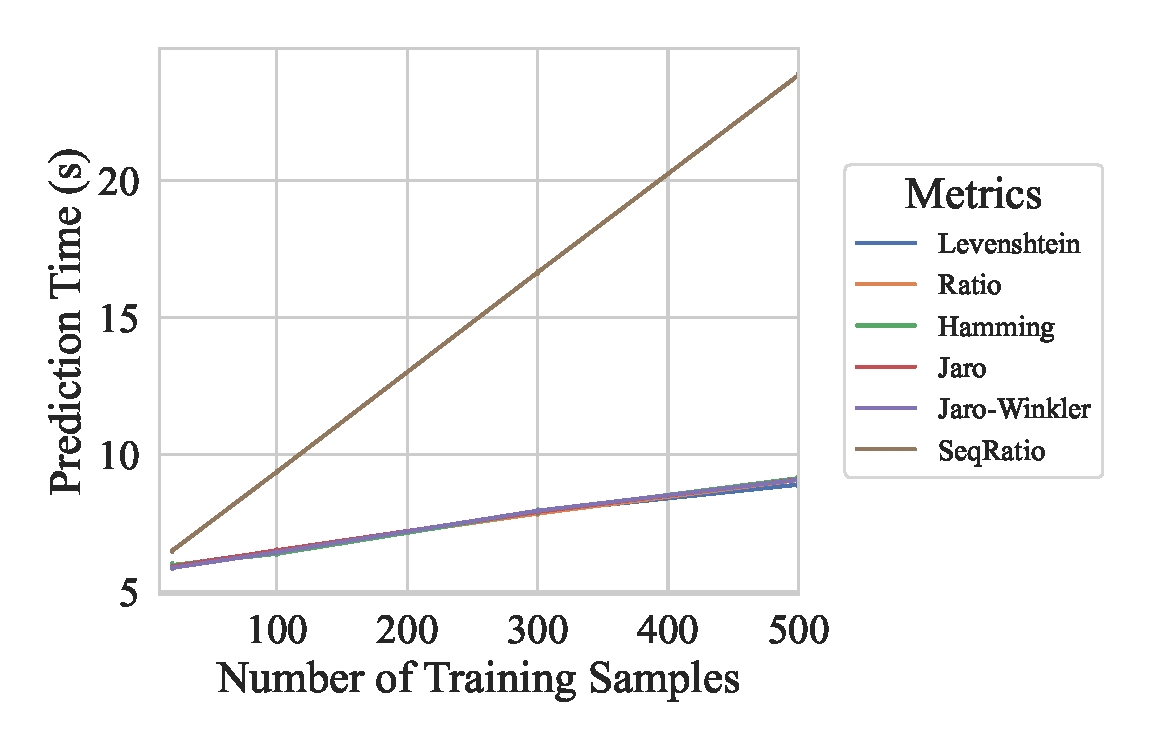
\includegraphics[width=\textwidth]{figs/sms_spam/string_metric_vs_predict_time.pdf}
	\end{subfigure}
	~
	\begin{subfigure}[t]{.44\textwidth}
		\centering
		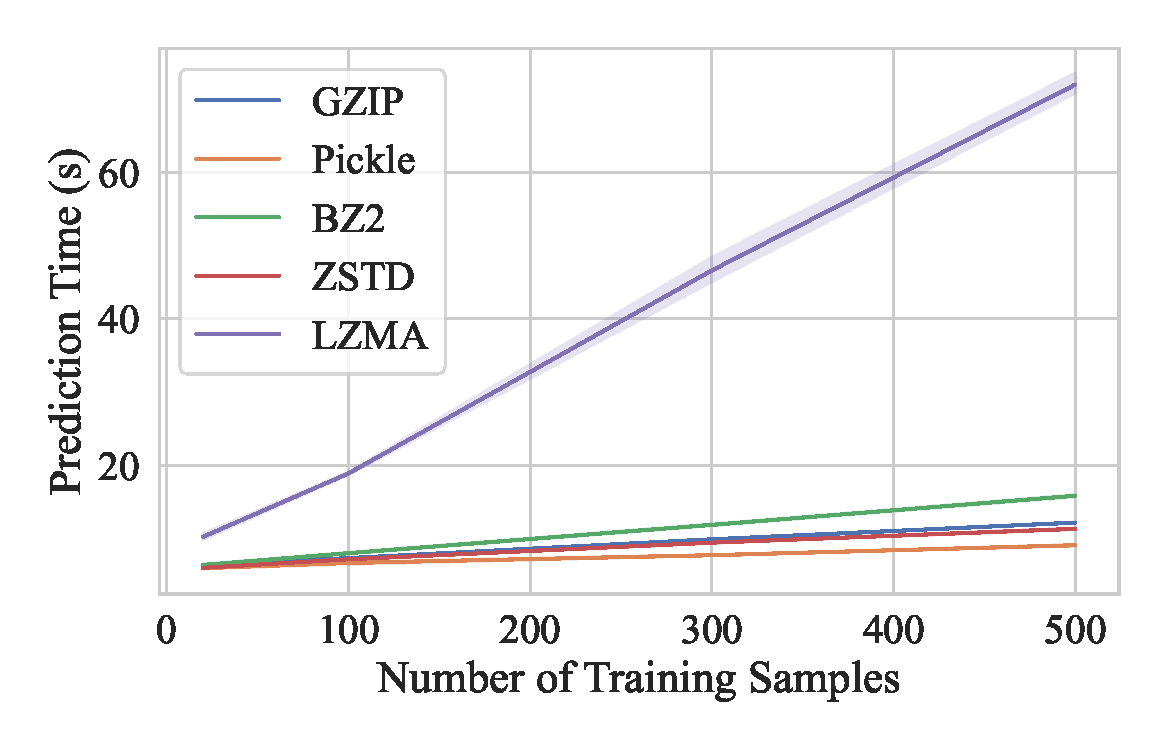
\includegraphics[width=\textwidth]{figs/sms_spam/compressor_metric_vs_predict_time.pdf}
	\end{subfigure}
	\caption{Prediction time across different different string metrics (left), and compression methods (right).}.
	\label{fig:sms_spam_prediction_time}
 
\end{figure}

\subsubsection{Symmetry}

Figure~\ref{fig:sms_spam_symmetry} shows the 

\begin{figure}[h!]
    \centering
    \captionsetup[subfigure]{skip=0pt}
    \begin{subfigure}[t]{.44\textwidth}
        \centering
        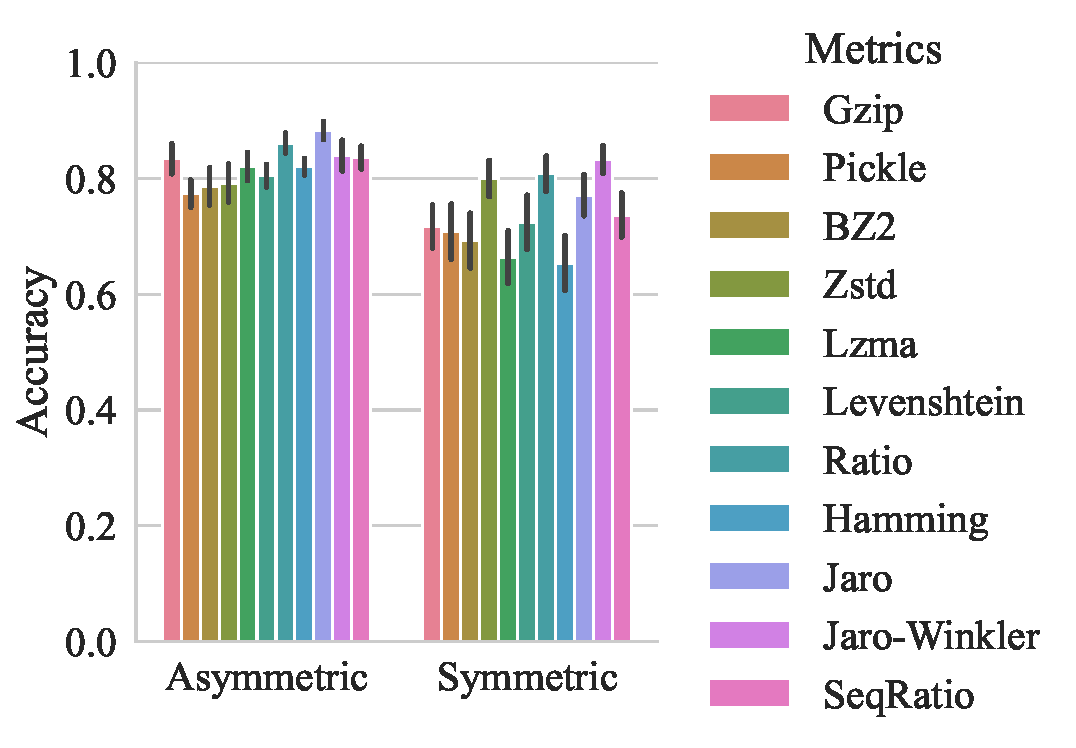
\includegraphics[width=\textwidth]{figs/sms_spam/symmetric_vs_metric.pdf}
    \end{subfigure}
    \begin{subfigure}[t]{.44\textwidth}
        \centering
        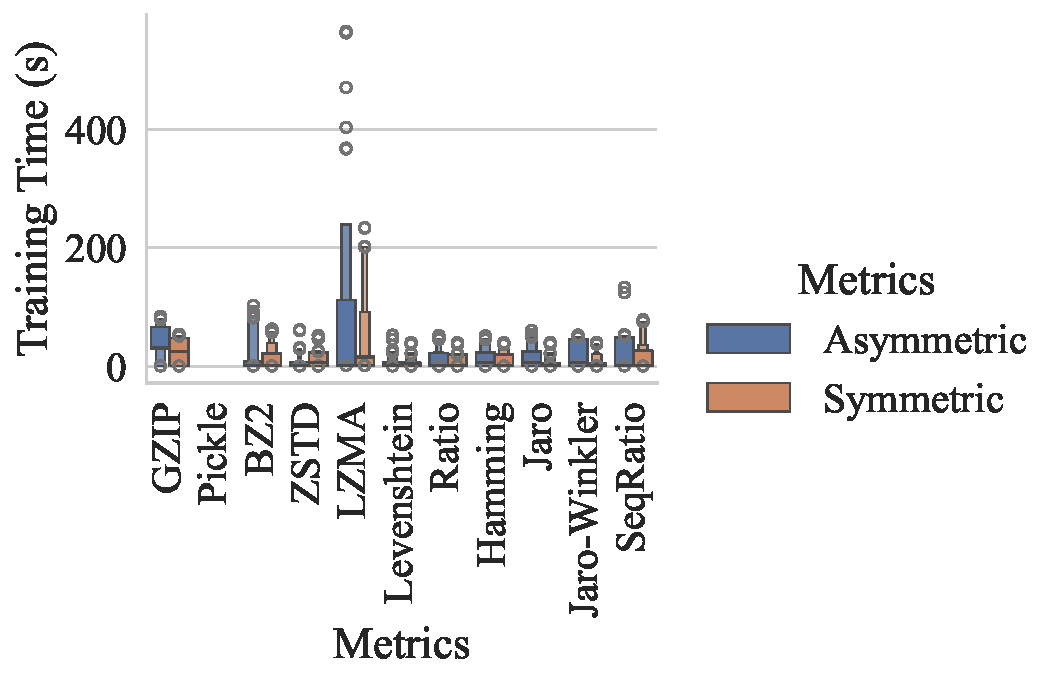
\includegraphics[width=\textwidth]{figs/sms_spam/symmetric_vs_metric_train_time.pdf}
    \end{subfigure}
    \caption{Accuracy across (left) and prediction time (right) across several compression methods and distance metrics with and without assuming symmetric distances.}
    \label{fig:sms_spam_symmetry}
\end{figure}
% \clearpage
% \subsection{KDD NSL}
This subsection reveals more granular data about the KDD NSL dataset.

\subsubsection{Accuracy}
Figure~\ref{fig:kdd_nsl_accuracy} shows the accuracy of different compressors, metrics, and sample selection methods.

\begin{figure}[h!][h]
	\centering
    \captionsetup[subfigure]{skip=0pt}
	\begin{subfigure}[t]{.44\textwidth}
		\centering
		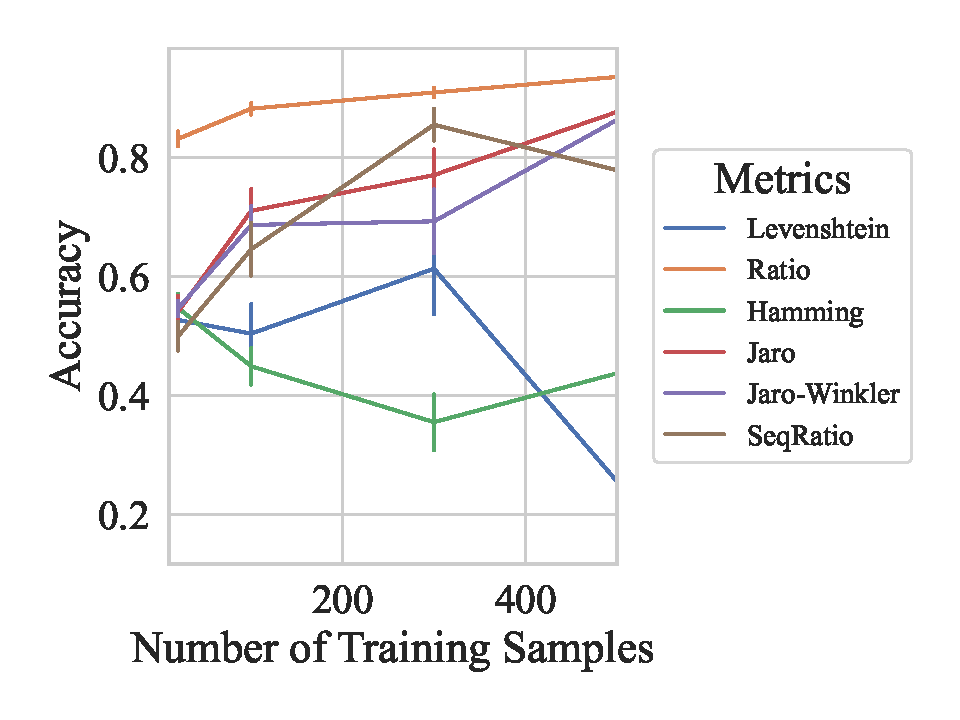
\includegraphics[width=\textwidth]{figs/kdd_nsl/string_metric_vs_accuracy.pdf}
	\end{subfigure}
	~
	\begin{subfigure}[t]{.44\textwidth}
		\centering
		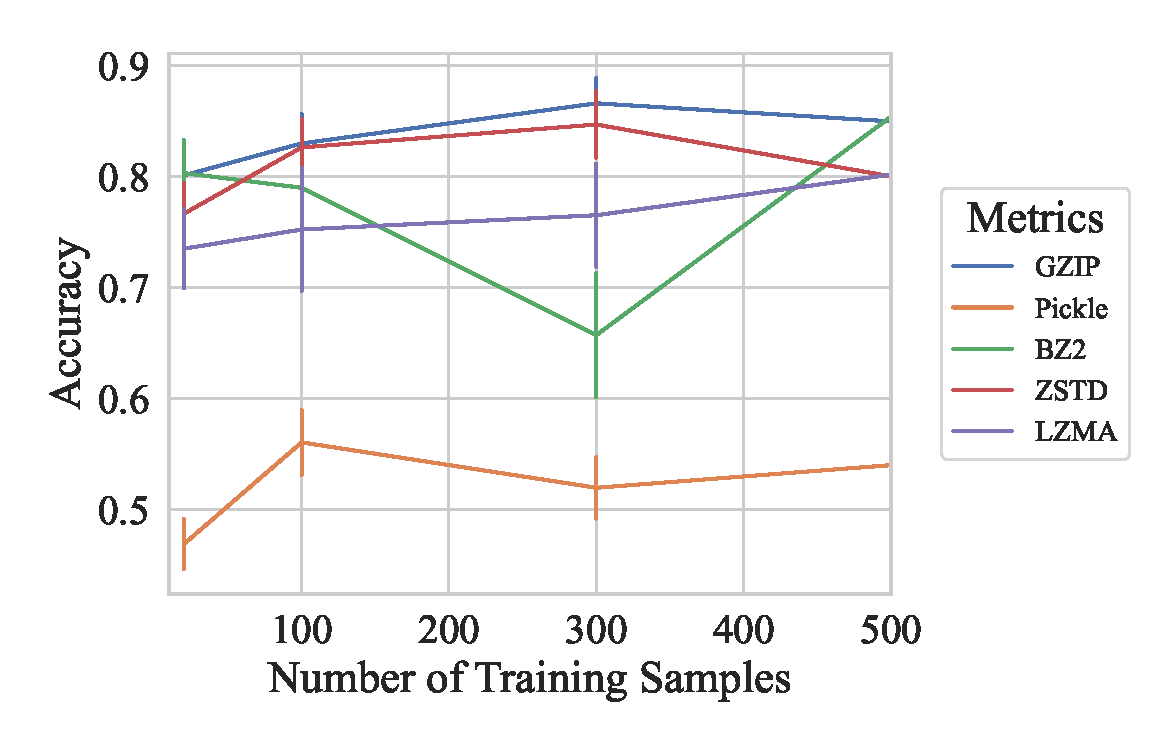
\includegraphics[width=\textwidth]{figs/kdd_nsl/compressor_metric_vs_accuracy.pdf}
	\end{subfigure}
	\caption{Accuracy across different different string kernel metrics (left), and compression methods (right).}
	\label{fig:kdd_nsl_accuracy}
\end{figure}

\subsubsection{Training Time}

Figure~\ref{fig:kdd_nsl_training_time} depicts the training time across all the tested compressors, distance metrics, and sample selection methods.

\begin{figure}[h!]
    \centering
    \captionsetup[subfigure]{skip=0pt}
	\begin{subfigure}[t]{.44\textwidth}
		\centering
		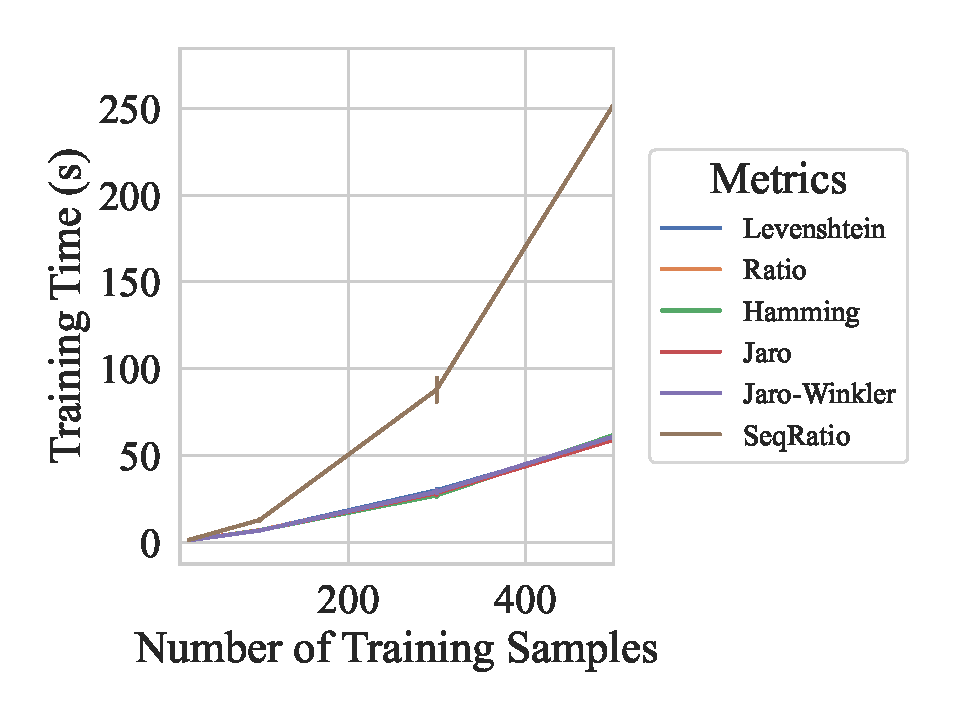
\includegraphics[width=\textwidth]{figs/kdd_nsl/string_metric_vs_train_time.pdf}
	\end{subfigure}
	~
	\begin{subfigure}[t]{.44\textwidth}
		\centering
		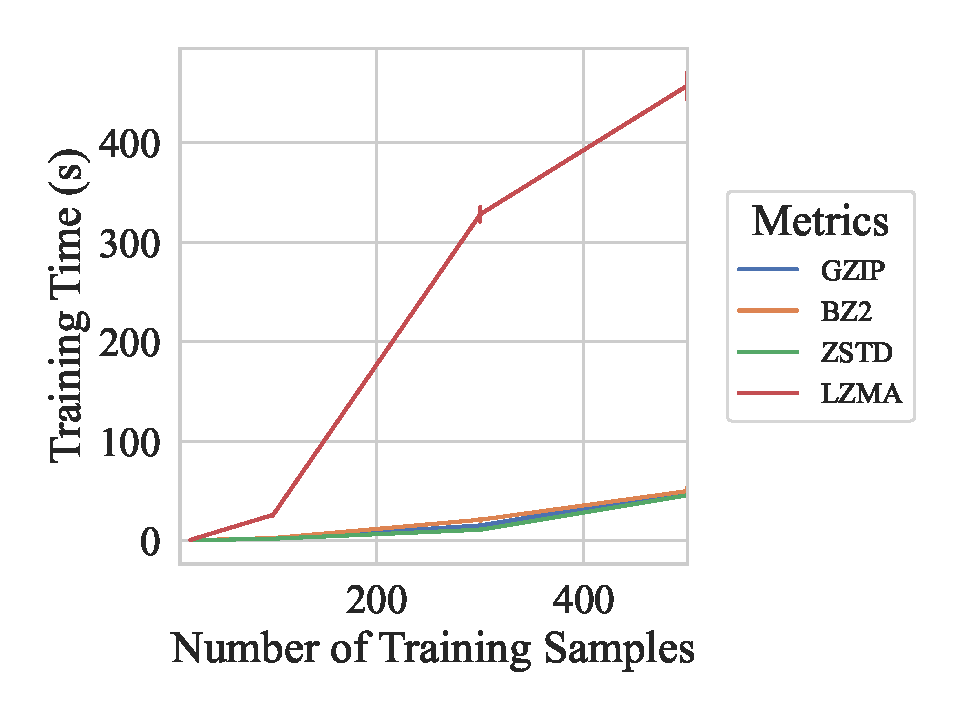
\includegraphics[width=\textwidth]{figs/kdd_nsl/compressor_metric_vs_train_time.pdf}
	\end{subfigure}
	\caption{Training time across different different string  metrics (left), and compression methods (right).}
	\label{fig:kdd_nsl_training_time}
\end{figure}

\subsubsection{Prediction Time}

Figure~\ref{fig:kdd_nsl_prediction_time} shows the prediction time of different compressors, metics, and sample selection methods.
\begin{figure}[h!]
	\centering
    \captionsetup[subfigure]{skip=0pt}
	\begin{subfigure}[t]{.44\textwidth}
		\centering
		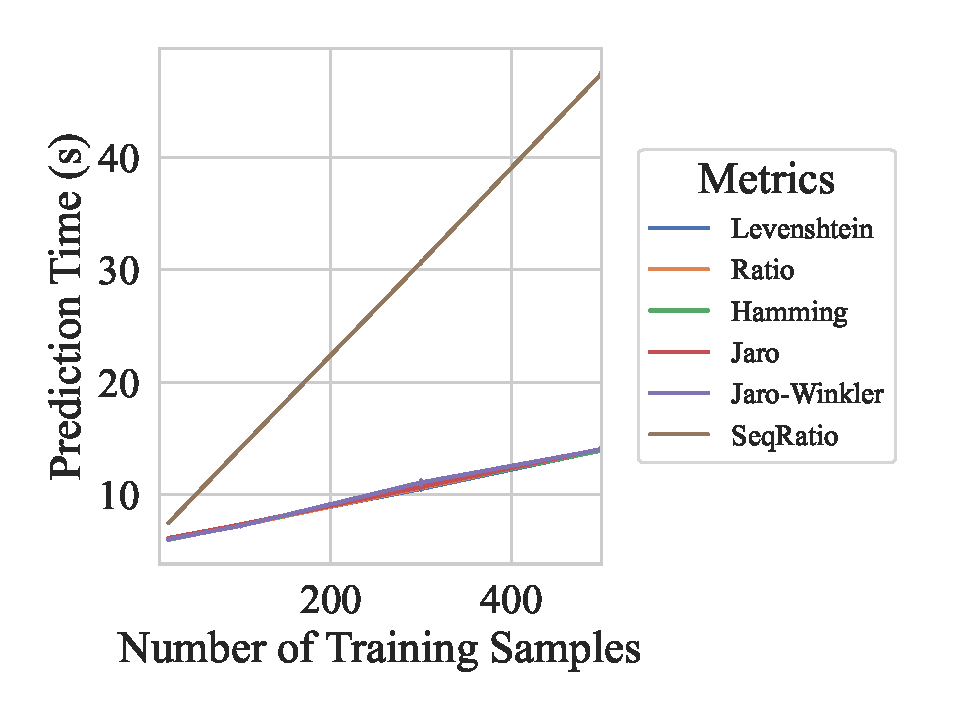
\includegraphics[width=\textwidth]{figs/kdd_nsl/string_metric_vs_predict_time.pdf}
	\end{subfigure}
	~
	\begin{subfigure}[t]{.44\textwidth}
		\centering
		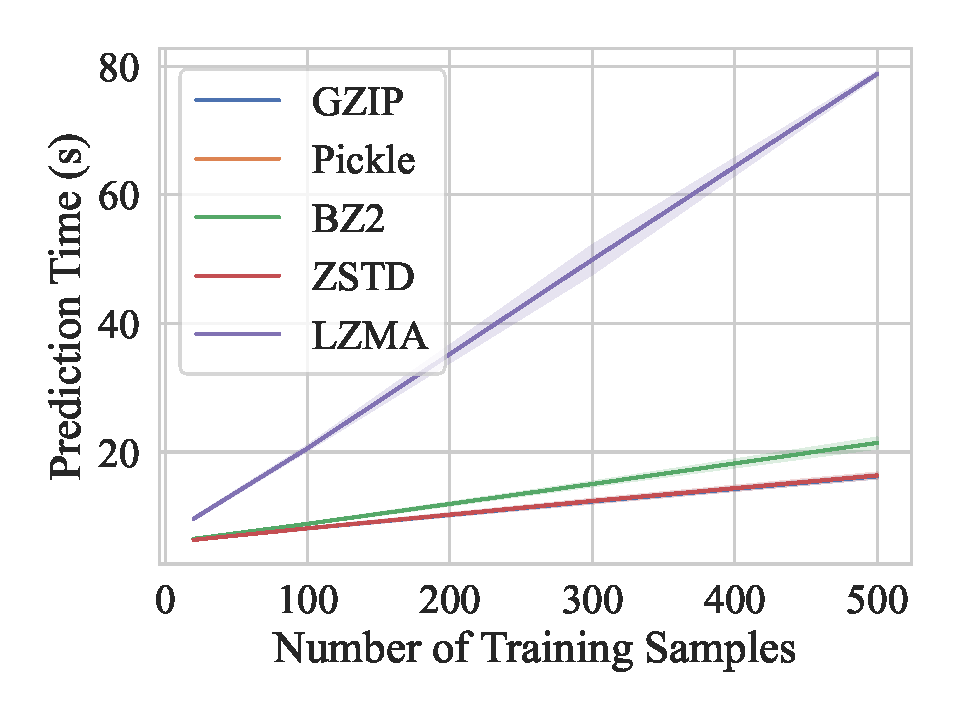
\includegraphics[width=\textwidth]{figs/kdd_nsl/compressor_metric_vs_predict_time.pdf}
	\end{subfigure}
	\caption{Prediction time across different different string metrics (left), and compression methods (right).}.
	\label{fig:kdd_nsl_prediction_time}
 
\end{figure}

\subsubsection{Symmetry}

Figure~\ref{fig:kdd_nsl_symmetry} shows the 

\begin{figure}[h!]
    \centering
    \captionsetup[subfigure]{skip=0pt}
    \begin{subfigure}[t]{.44\textwidth}
        \centering
        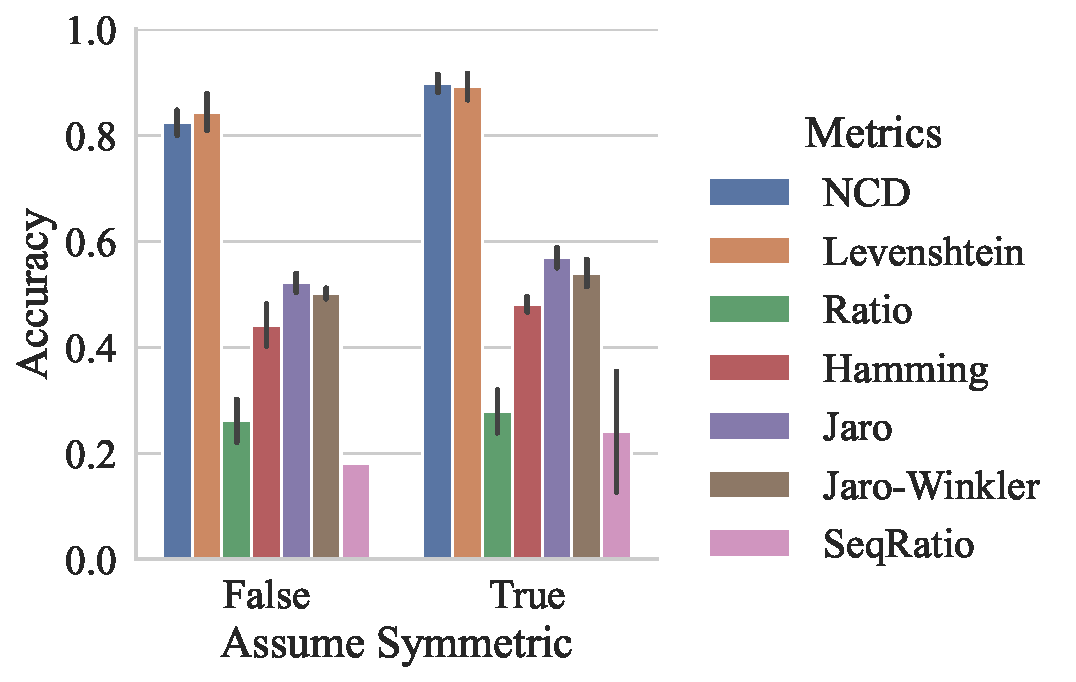
\includegraphics[width=\textwidth]{figs/kdd_nsl/symmetric_vs_metric.pdf}
    \end{subfigure}
    \begin{subfigure}[t]{.44\textwidth}
        \centering
        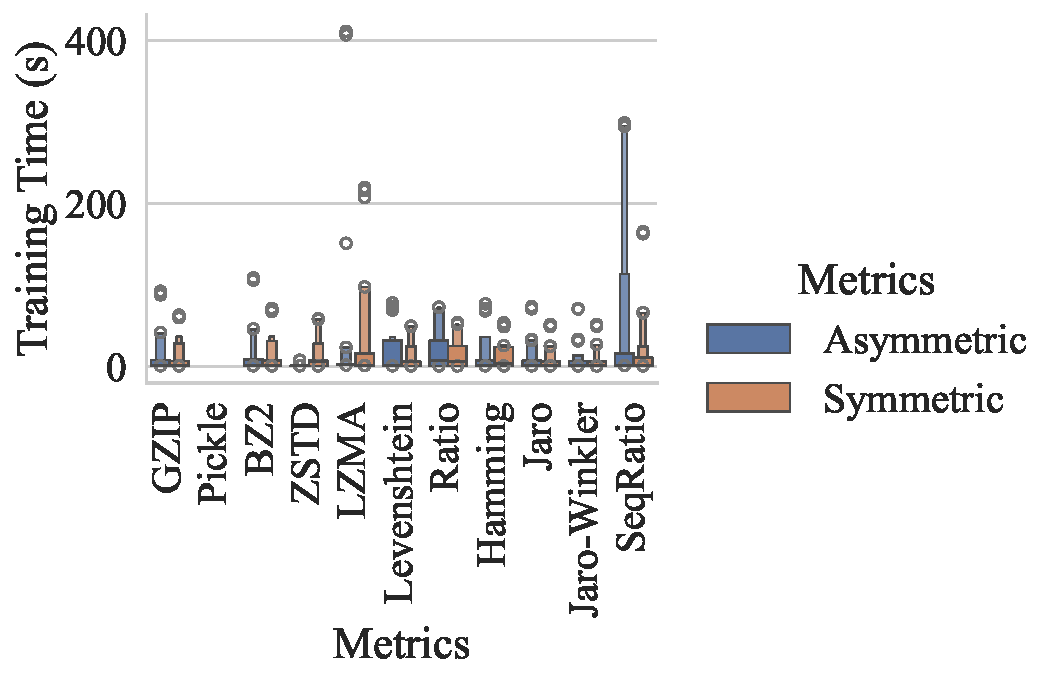
\includegraphics[width=\textwidth]{figs/kdd_nsl/symmetric_vs_metric_train_time.pdf}
    \end{subfigure}
    \caption{Accuracy across (left) and prediction time (right) across several compression methods and distance metrics with and without assuming symmetric distances.}
    \label{fig:kdd_nsl_symmetry}
\end{figure}
% \clearpage
% \subsection{Truthseeker}
This subsection reveals more granular data about the Truthseeker dataset.

\subsubsection{Accuracy}
Figure~\ref{fig:truthseeker_accuracy} shows the accuracy of different compressors, metrics, and sample selection methods.

\begin{figure}[h!][h]
	\centering
    \captionsetup[subfigure]{skip=0pt}
	\begin{subfigure}[t]{.44\textwidth}
		\centering
		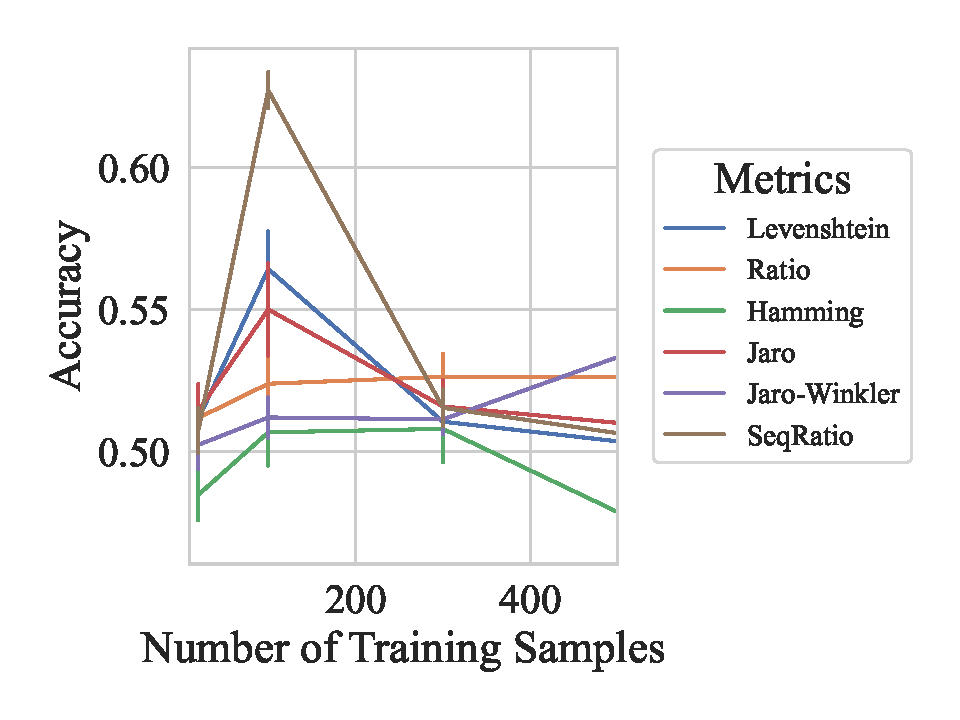
\includegraphics[width=\textwidth]{figs/truthseeker/string_metric_vs_accuracy.pdf}
	\end{subfigure}
	~
	\begin{subfigure}[t]{.44\textwidth}
		\centering
		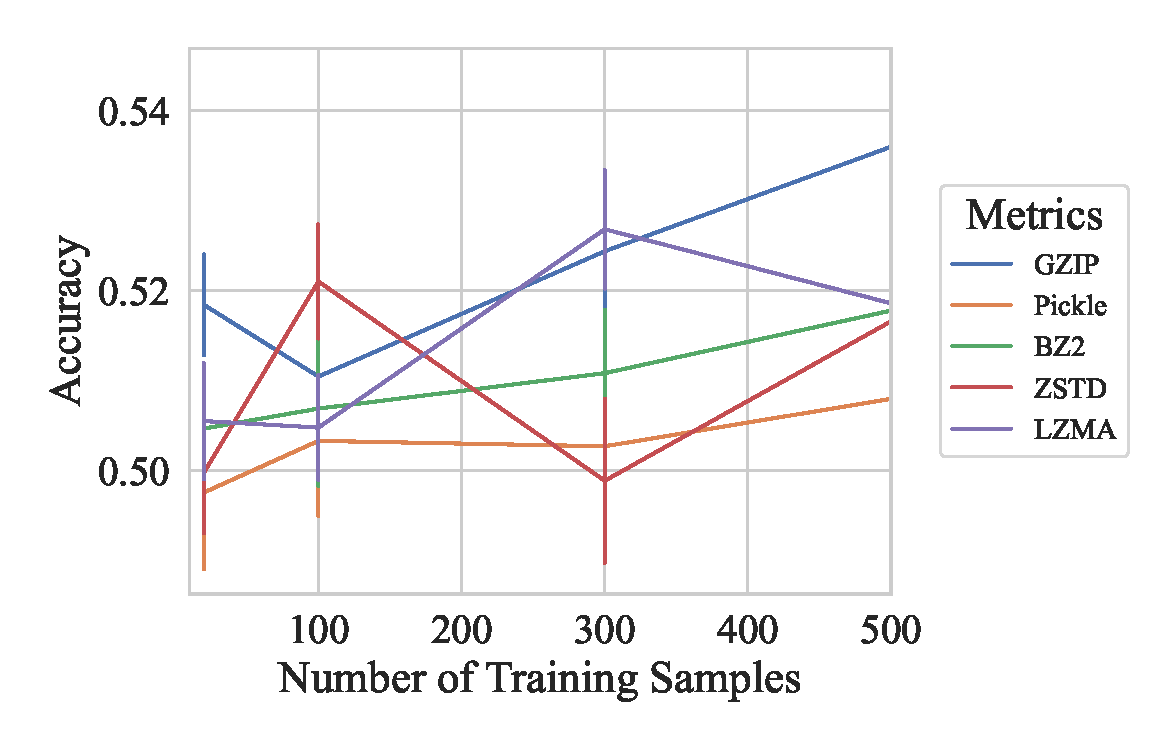
\includegraphics[width=\textwidth]{figs/truthseeker/compressor_metric_vs_accuracy.pdf}
	\end{subfigure}
	\caption{Accuracy across different different string kernel metrics (left), and compression methods (right).}
	\label{fig:truthseeker_accuracy}
\end{figure}

\subsubsection{Training Time}

Figure~\ref{fig:truthseeker_training_time} depicts the training time across all the tested compressors, distance metrics, and sample selection methods.

\begin{figure}[h!]
    \centering
    \captionsetup[subfigure]{skip=0pt}
	\begin{subfigure}[t]{.44\textwidth}
		\centering
		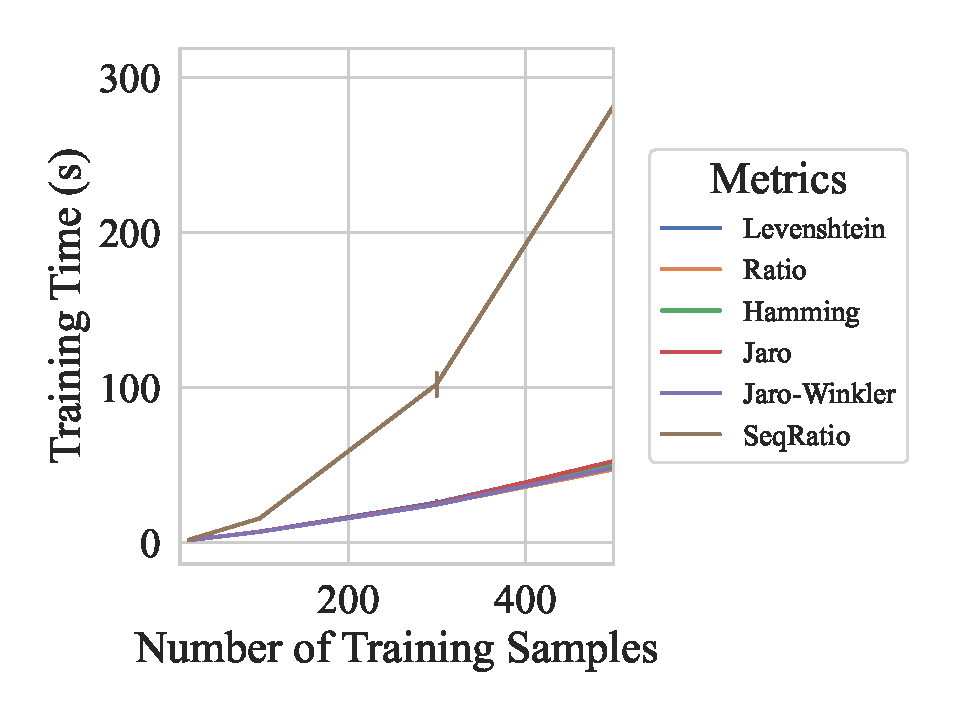
\includegraphics[width=\textwidth]{figs/truthseeker/string_metric_vs_train_time.pdf}
	\end{subfigure}
	~
	\begin{subfigure}[t]{.44\textwidth}
		\centering
		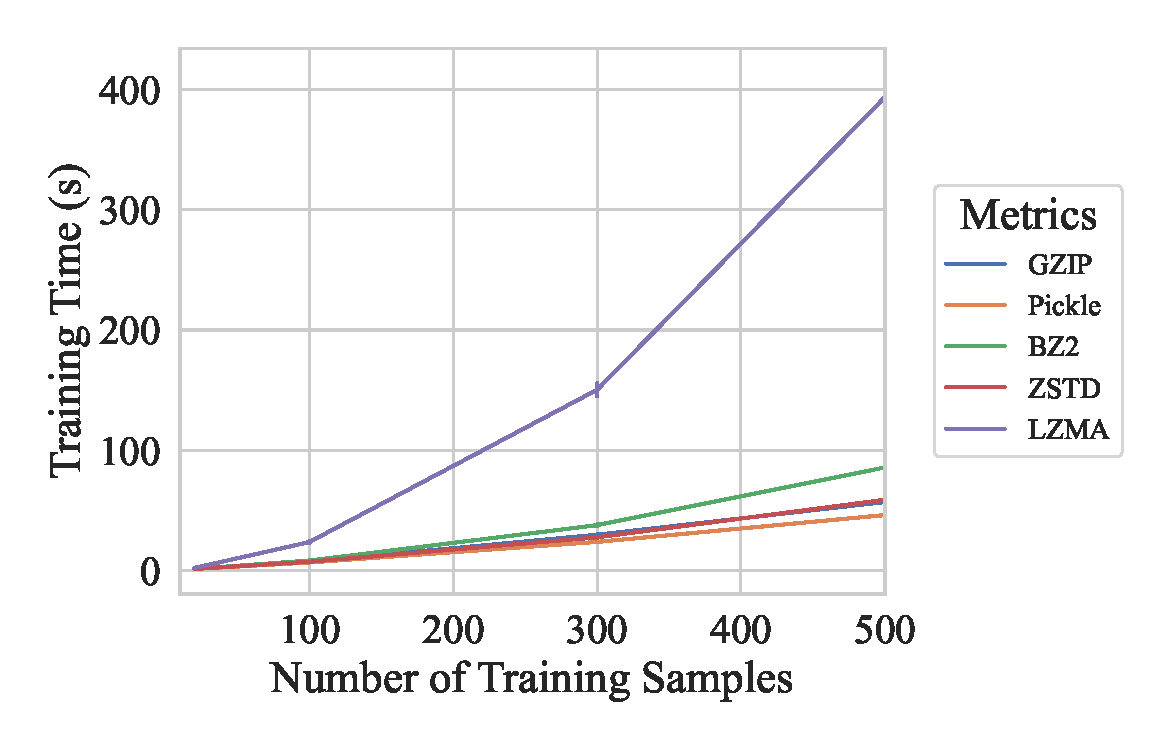
\includegraphics[width=\textwidth]{figs/truthseeker/compressor_metric_vs_train_time.pdf}
	\end{subfigure}
	\caption{Training time across different different string  metrics (left), and compression methods (right).}
	\label{fig:truthseeker_training_time}
\end{figure}

\subsubsection{Prediction Time}

Figure~\ref{fig:truthseeker_prediction_time} shows the prediction time of different compressors, metics, and sample selection methods.
\begin{figure}[h!]
	\centering
    \captionsetup[subfigure]{skip=0pt}
	\begin{subfigure}[t]{.44\textwidth}
		\centering
		\includegraphics[width=\textwidth]{figs/truthseeker/string_metric_vs_predict_time.pdf}
	\end{subfigure}
	~
	\begin{subfigure}[t]{.44\textwidth}
		\centering
		\includegraphics[width=\textwidth]{figs/truthseeker/compressor_metric_vs_predict_time.pdf}
	\end{subfigure}
	\caption{Prediction time across different different string metrics (left), and compression methods (right).}.
	\label{fig:truthseeker_prediction_time}
 
\end{figure}

\subsubsection{Symmetry}

Figure~\ref{fig:truthseeker_symmetry} shows the 

\begin{figure}[h!]
    \centering
    \captionsetup[subfigure]{skip=0pt}
    \begin{subfigure}[t]{.44\textwidth}
        \centering
        \includegraphics[width=\textwidth]{figs/truthseeker/symmetric_vs_metric.pdf}
    \end{subfigure}
    \begin{subfigure}[t]{.44\textwidth}
        \centering
        \includegraphics[width=\textwidth]{figs/truthseeker/symmetric_vs_metric_train_time.pdf}
    \end{subfigure}
    \caption{Accuracy across (left) and prediction time (right) across several compression methods and distance metrics with and without assuming symmetric distances.}
    \label{fig:truthseeker_symmetry}
\end{figure}

\end{document}
